%The EPL master thesis cover template
\documentclass[twoside,openright]{eplmastersthesis}

% Fill in here the information: title, student name, speciality, jury members
\title{Title of the master thesis}	% Master thesis title
\subtitle{Subtitle (optional)}			% Optional subtitle
\author{Firstname \textsc{Lastname}}	% Student name
\secondauthor{Firstname \textsc{Lastname}}	% Second student name if applicable
\speciality{Speciality}		% Speciality (use one of the following options):
										% Biomedical Engineering
										% Chemical and Materials Engineering
										% Civil Engineering
										% Computer Science
										% Computer Science and Engineering
										% Electrical Engineering
										% Electro-mechanical Engineering
										% Mathematical Engineering
										% Mechanical Engineering
										% Physical Engineering
%\options{Option(s)}		% If required by program commission mention options
\supervisor{Firstname \textsc{Lastname}}	% 1st supervisor name
\cosupervisor{Firstname \textsc{Lastname}}	% 2nd supervisor name if applicable
\readerone{Firstname \textsc{Lastname}}		% 1st reader name
\readertwo{Firstname \textsc{Lastname}}		% 2nd reader name
\readerthree{Firstname \textsc{Lastname}}	% 3rd reader name
\years{20..-20..}	% Academic year

\begin{document}

\maketitle					% To create front cover page
%\thispagestyle{empty}		% To suppress header and footer on the back of the cover page
\newpage\null\thispagestyle{empty}\newpage % Blank page

\pagestyle{fancy}

\pagenumbering{arabic}

\chapter{Theory}

This is the intro. 
\section{Presentation of the problem}

In this section, we will present the problem we will solve. Let us consider a domain $\Omega \in \mathbb{R}^2$ with its boundary $\Gamma = \partial\Omega$. Then, we want to find a function $u : \Omega \rightarrow \mathbb{R}$ that satisfies : 

\begin{align}
\nabla^2 u &= f &\text{on $\Omega$} \label{eq:poisson}\\
u &= u_0 &\text{on $\Gamma$}
\end{align}

Where $f : \Omega \rightarrow \mathbb{R}$ and $u_0 : \Gamma \rightarrow \mathbb{R}$ are two given functions. We also assume that $f$ and $u_0$ satisfy the standard regularity assumptions. Let us denote $H^1(\Omega)$, the Sobolev space containing functions whose partial derivatives up to order 1 are in $L^2(\Omega)$. Let us also define $H^1_0(\Omega)$, a subspace of $H^1(\Omega)$ where the functions are equal to zero on $\Gamma$. 

\begin{align*}
H_0^1(\Omega) = \{ v \in H^1(\Omega) , v|_\Gamma = 0 \}
\end{align*}

Let us then multiply equation \ref{eq:poisson} by any function $v$ in $H_0^1(\Omega)$ and  integrate it over the domain. And since the laplacian is equivalent to the divergence of the gradient, we have that : 

\begin{align}
\int_\Omega \nabla \cdot (\nabla u)v \:dxdy = \int_\Omega f v \:dxdy \label{eq:sobolev}
\end{align}

Any function $u$ that is a solution of \ref{eq:poisson} is obviously also a solution of \ref{eq:sobolev} for every function $v \in H_0^1(\Omega)$. Let us now recall that for any functions $u$ and $v$ regular enough : 

$$\nabla \cdot (v\nabla u) = \nabla u \cdot \nabla v + v\nabla \cdot (\nabla u)$$

Using this relation on equation \ref{eq:sobolev}, we get : 

\begin{align}
\int_\Omega \nabla u \cdot \nabla v \:dxdy = -\int_\Omega \nabla \cdot (v\nabla u) dxdy -\int_\Omega f v \:dxdy
\end{align}

Finally, using the divergence theorem, we have : 

\begin{align}
\int_\Omega \nabla u \cdot \nabla v \:dxdy = -\int_\Gamma (v\nabla u) \cdot \textbf{n} \:ds -\int_\Omega f v \:dxdy
\end{align}

Since $v\in H_0^1(\Omega)$, it is equal to zero on the boundary and therefore : 

\begin{align}
\int_\Omega \nabla u \cdot \nabla v \:dxdy = -\int_\Omega f v \:dxdy 
\end{align}

We can now state the weak formulation of problem \ref{eq:poisson}. Let us assume, without loss of generality that $u_0 = 0$. Then, we want to find a function $u \in H^1_0(\Omega)$ that satisfies : 

\begin{align}
\int_\Omega \nabla u \cdot \nabla v \:dxdy &= -\int_\Omega f v \:dxdy &\forall v \in H_0^1(\Omega) \label{eq:weakform} 
\end{align}

 
\section{Spectral element method on non conforming meshes}
Equation \ref{eq:weakform} is the problem we will be attempting to solve. However, the equation must still hold for every function $v \in H_0^1(\Omega)$. This section presents the method used for the discretization of the problem, namely the spectral element method on a non conforming mesh. 

The first part of the task is the discretization of the domain $\Omega$. As explained in the introduction, we will use non conforming meshes. So we will present such meshes, present their particularities and explain how we will handle them.   

The second part of the task is the discretization of equation \ref{eq:weakform}. The method here presented is the spectral element method, which consists of using high degree piece-wise polynomials as basis functions. We will first show how to obtain the linear system of equation ($Au=b$) that arises with this method. We will afterwards present the one dimensional basis functions used and the location of the nodes on the 1D reference element. We will then explain how to construct the global basis functions in the presence of hanging nodes. We will finally show how to compute the right hand side of the linear system and how to perform an efficient matrix-vector product without having to explicitly construct the matrix $A$.

\subsection{Discretization of the domain}

Let us first tackle the discretization of the domain. In classical AMR, the mesh depends on the problem to solve and the refinement is performed to obtain the fact that the error committed on each quadrant is roughly the same (\textcolor{red}{ref here}). But that is not the focus of the work done here. Instead, let us assume that we already have a mesh $G$ consisting of unstructured quadrilaterals (denoted $\Omega_e$) and that might be non conforming, i.e. where we have the presence of hanging nodes. As always, we have : 

\begin{align*}
G &= \bigcup\limits_{e} \Omega_e\\
\Omega_i \cap \Omega_j &= \emptyset &\text{if $i\neq j$}
\end{align*}

\begin{figure}
\centering
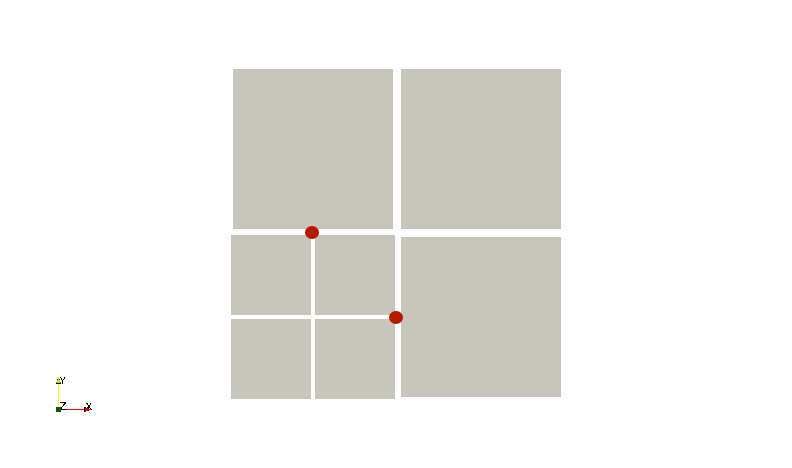
\includegraphics[scale=0.45]{Theory/hang_ex.png}
\caption{Example of a legal non conforming mesh (it is 1-irregular). We can see that we have two hanging nodes in red since they are not vertices of the bigger quadrants neighboring them.}
\label{hang_ex}
\end{figure}

We can define a hanging node as being a node that is not shared between all its neighboring quadrants. We can note that hanging nodes can only be found on edges. Figure \ref{hang_ex} shows an example of a mesh containing hanging nodes. We can see that the vertices in red are hanging nodes since they are vertices of the smaller quadrants neighboring them but not of the bigger quadrants neighboring them. Those nodes will require a special treatment in the spectral element method. 

\begin{figure}
\centering
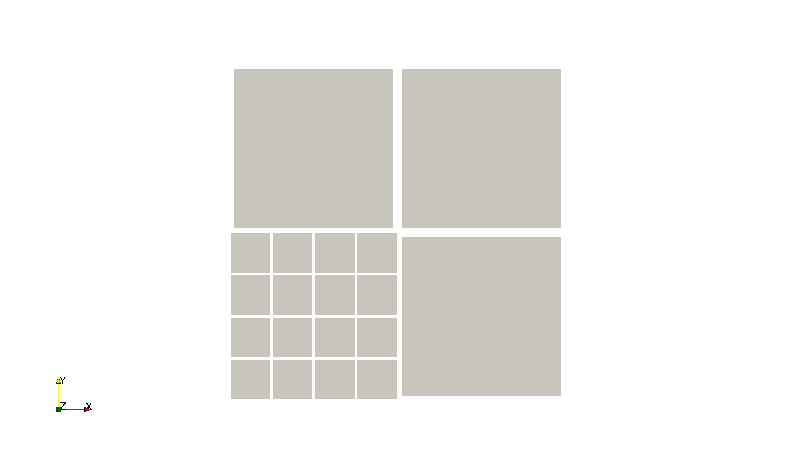
\includegraphics[scale=0.45]{Theory/hang_illegal.png}
\caption{Example of an illegal non conforming mesh (it is 2-irregular). We can see that the top left quadrant has four neighbors through its south edge while we imposed a maximum of two. }
\label{hang_illegal}
\end{figure}

We have however one restriction to make on the mesh. We will allow two neighboring quadrants to have only one level of difference in the refinement. This means that the number of neighbors of a quadrant through a given edge is maximum two. We call such meshes 1-irregular. Figure \ref{hang_illegal} shows an example of an illegal non conforming mesh. We can see that on that mesh the top left quadrant has four neighbors through its south edge. Since the maximum difference of the levels of refinement between two neighboring quadrants is two, such a mesh is called 2-irregular.  Handling all possibilities of hanging faces for a general $k$-irregular mesh (with $k>1$) is impossible and that is why we (and the vast majority of others) consider as illegal meshes such as the one presented in figure \ref{hang_illegal}.

For the rest of this chapter, it is important to note that, in a 1-irregular mesh, a hanging edge (an edge containing hanging nodes) is always half of a non hanging edge for its neighboring quadrant.

Once we have our mesh, it is clear that we can compute the integral of any scalar function $g$ as the sum of integrals on the quadrants. Formally, we have :  

\begin{align}
\int_\Omega g\:dxdy = \sum_e \int_{\Omega_e} g\:dxdy \label{eq:int}
\end{align}

All the integrals we compute will be performed quadrant by quadrant and then summed. 

\subsection{Discretization of equation \ref{eq:weakform}}

Since equation \ref{eq:weakform} must hold for every function $v \in H_0^1(\Omega)$, it is not very practical. We will therefore restrict ourselves to $V^h \subset H_0^1(\Omega)$, where $V^h$ has a finite dimension. Let us denote the functions that form the basis of $V^h$ by $\phi_1,..., \phi_N$ (therefore, the space $V^h$ is of dimension $N$). We will define explicitly those basis functions later. 

Using Galerkin approximation, we will also restrict our search of the solution to $V^h$. Let us denote this solution $u^h$. Therefore, we have that : 

$$u^h = \sum_{j=1}^N u_j \phi_j $$

Asking equation \ref{eq:weakform} to be satisfied for every function in $V^h$ is equivalent to ask it to be satisfied for every function of its basis. As a result, the discretized version of equation \ref{eq:weakform} is given by : 

\begin{align}
\sum_{j = 1}^N \int_\Omega \nabla \phi_i \cdot \nabla \phi_j \:dxdy \: u_j &= -\int_\Omega f\phi_i \:dxdy &\text{for $i=1,...,N$} 
\end{align}

Solving this to get the nodal values $u_j$ is actually solving a linear system of equations $\textbf{Au}=\textbf{b}$ where we define : 

\begin{align}
A_{ij} &= \int_\Omega \nabla \phi_i \cdot \nabla \phi_j \:dxdy \label{eq:A}\\
b_i &= -\int_\Omega f\phi_i \:dxdy \label{eq:b}
\end{align}

Those integral will be performed using equation \ref{eq:int}.

\subsection{Basis functions on the reference element and Gauss-Lobatto-Legendre nodes}

As shows equations \ref{eq:A} and \ref{eq:b}, we need to compute integrals to solve the problem. Here, we will perform the integration using Gauss-Lobatto-Legendre (GLL) quadrature. The particularity of 1D GLL nodes is that they include the end points of the interval on which we compute the integral. For example, on the one dimensional reference element, it means that the GLL nodes include $\xi = -1$ and $\xi=1$. This particularity enables us to use the GLL nodes both as quadrature points and as global nodes where we compute our numerical solution. We will see later that this allows us to compute the matrix-vector product very efficiently. 

For $p+1$ GLL nodes, the quadrature integrate exactly polynomials of degree at most $2p-1$. It is less than for the Gauss-Legendre quadrature (which achieve to integrate exactly polynomials up to order $2p+1$). The way to compute the GLL nodes and their weights is for example detailled in \cite{gll_nodes}. Table \ref{gll_values} shows the values for different degrees. We can see that the nodes are not uniformly distributed but they tend to cluster near the end points $\xi = -1$ and $\xi=1$.

\begin{table}
\centering
\begin{tabular}{c|cc}
\hline
 Number of nodes $p+1$ & Points $\xi_i$ & Weights $w_i$\\
 \hline
 2 & $\pm 1$ & $1$ \\
 \hline
 3 & $\pm 1$ & $\frac{1}{3}$\\
    & 0			   & $\frac{4}{3}$\\
 \hline
 4 & $\pm 1$ & $\frac{1}{6}$\\
    & $\pm \sqrt{\frac{1}{5}}$  & $\frac{5}{6}$\\
\hline
5 & $\pm 1$ & $\frac{1}{10}$\\
   & $\pm \sqrt{\frac{3}{7}}$ & $\frac{49}{90}$\\
   & $0$ & $\frac{32}{45}$\\
   \hline
\end{tabular}
\caption{Values of the GLL nodes and the associated weights on the reference one dimensional element for the first few degrees.}
\label{gll_values}
\end{table}

Let us denote the $p+1$ GLL nodes on the reference 1D element by $\xi_0$, $\xi_1$, ..., $\xi_p$. Since the GLL nodes contain the end points of the interval, we can also use them as global nodes. We will use Lagrangian polynomials for the interpolation. Let us denote them $l_0(\xi)$, $l_1(\xi)$, ... , $l_p(\xi)$. Let us recall that : 

$$ l_i(\xi) = \prod_{j=0 , j\neq i}^p \frac{\xi - \xi_j}{\xi_i  - \xi_j}$$

For the following parts of this chapter, it is very important to note that :

$$ l_i(\xi_j) = \delta_{ij} $$ 

Where $\delta_{ij}$ is to be understood as the Kronecker delta. This fact will allow us later to compute the matrix-vector product in a very efficient way. 

Let us also use this opportunity to define the derivation matrix $H$ as : 

\begin{align}
H_{ij} = l_i'(\xi_j) \label{eq:derivation_matrix}
\end{align}

Let us now define the basis functions on the 2D reference element. In 2D, we will use $(p+1)^2$ nodes, tensor product of the 1D GLL nodes. If we denote the 1D GLL nodes by $\xi_i^1$, the 2D nodes are thus located at :

\begin{align*}
(\xi_i, \eta_j) &= (\xi^1_i,\xi^1_j) &\text{for $i,j=0,1,...,p$}
\end{align*}

On the reference quadrant $\xi, \eta \in [-1;1]$, we have in the same way that the basis function associated with node $I$ located at $(\xi_i,\eta_j)$ is given the tensor product of the 1D basis functions : 

$$\phi_I(\xi,\eta) = l_i(\xi)l_j(\eta)$$

Thus, if we want to obtain the value of a field $u$ in the reference quadrant, whose value at node $I$ is given by $u_{ij}$, we interpolate as : 

\begin{align*}
u(\xi,\eta) = \sum_{i=0}^p\sum_{j=0}^p u_{ij}l_i(\xi)l_j(\eta)
\end{align*}

\subsection{Global basis function}

Let us first mention the distinction between global and local nodes. Each quadrant has $(p+1)^2$ local GLL nodes but that does not mean that all of them are global nodes, since some might be hanging. As explained in \cite{hang_treat}, one solution consists to treat hanging nodes as global nodes and then add equations in the linear system $Au=b$ to enforce the continuity of the numerical solution. Another solution is to immediately enforce the continuity of the numerical solution by having continuous global basis function. This is what is done here. We will consider $N$ global nodes (that are the GLL nodes for at least one quadrant) and give them a global unique index $I = 1,...,N$. 

We want our global basis function $\phi_I$ to be a piece-wise polynomial of order $p$ and to have a value of exactly $1$ at global node $I$ and to be equal to $0$ on any other global node. 

In order to define such a function, we first need a mapping that goes from the 2D reference element to the actual quadrant $e$, i.e. $x^e(\xi,\eta)$ and $y^e(\xi,\eta)$ that for quadrant $e$ give the actual coordinates of any point in the reference element. Let us also define the inverse mappings $\xi^e(x,y)$ and $\eta^e(x,y)$. 

The last thing we need is a global to local operator that gives for local node $(\xi_i,\eta_j)$ on quadrant $e$ the weight of global node $I$. Let us denote this operator $R^e_{ij}(I)$. In a conforming mesh, since each local node correspond to a global node, $R^e_{ij}(I)$ can only be equal to 0 or to 1. In a non conforming mesh, however, the value of $R^e_{ij}(I)$ must be computed to ensure the continuity of the global basis function. For example, if we have hanging nodes on the east edge of quadrant $e$ (where $i=p$), then $R^e_{pj}(I)$ is given by : 

\begin{align*}
R^e_{pj}(I) &= l_k \left(\frac{\xi_j}{2}\pm \frac{1}{2}\right) &\text{if $I$ is the $k$-th global node on the non hanging east edge}
\end{align*} 

More explanation about how to compute the operator $R^e_{ij}(I)$ can be found in \cite{hang_handle}. The plus or minus sign in the above formula comes from the fact that a hanging edge can be the first or the second part of the larger non hanging edge. This is why we accept only 1-irregular meshes : because we only have to handle two cases when we compute $R^e_{ij}(I)$. If we accepted $k$-irregular meshes with $k>1$, we would have too many different cases to look at. 

With this operator and our mapping, it is then possible to compute the value of the basis function associated with node $I$ inside any element $e$. It is given by : 

\begin{align}
\phi_I(x,y) &= \sum_{i=0}^p\sum_{j=0}^p R^e_{ij}(I) \: l_i(\xi^e(x,y))\: l_j(\eta^e(x,y)) &\text{if $(x,y) \in \Omega_e$}\label{eq:global_basis}
\end{align}

\begin{figure}
\centering
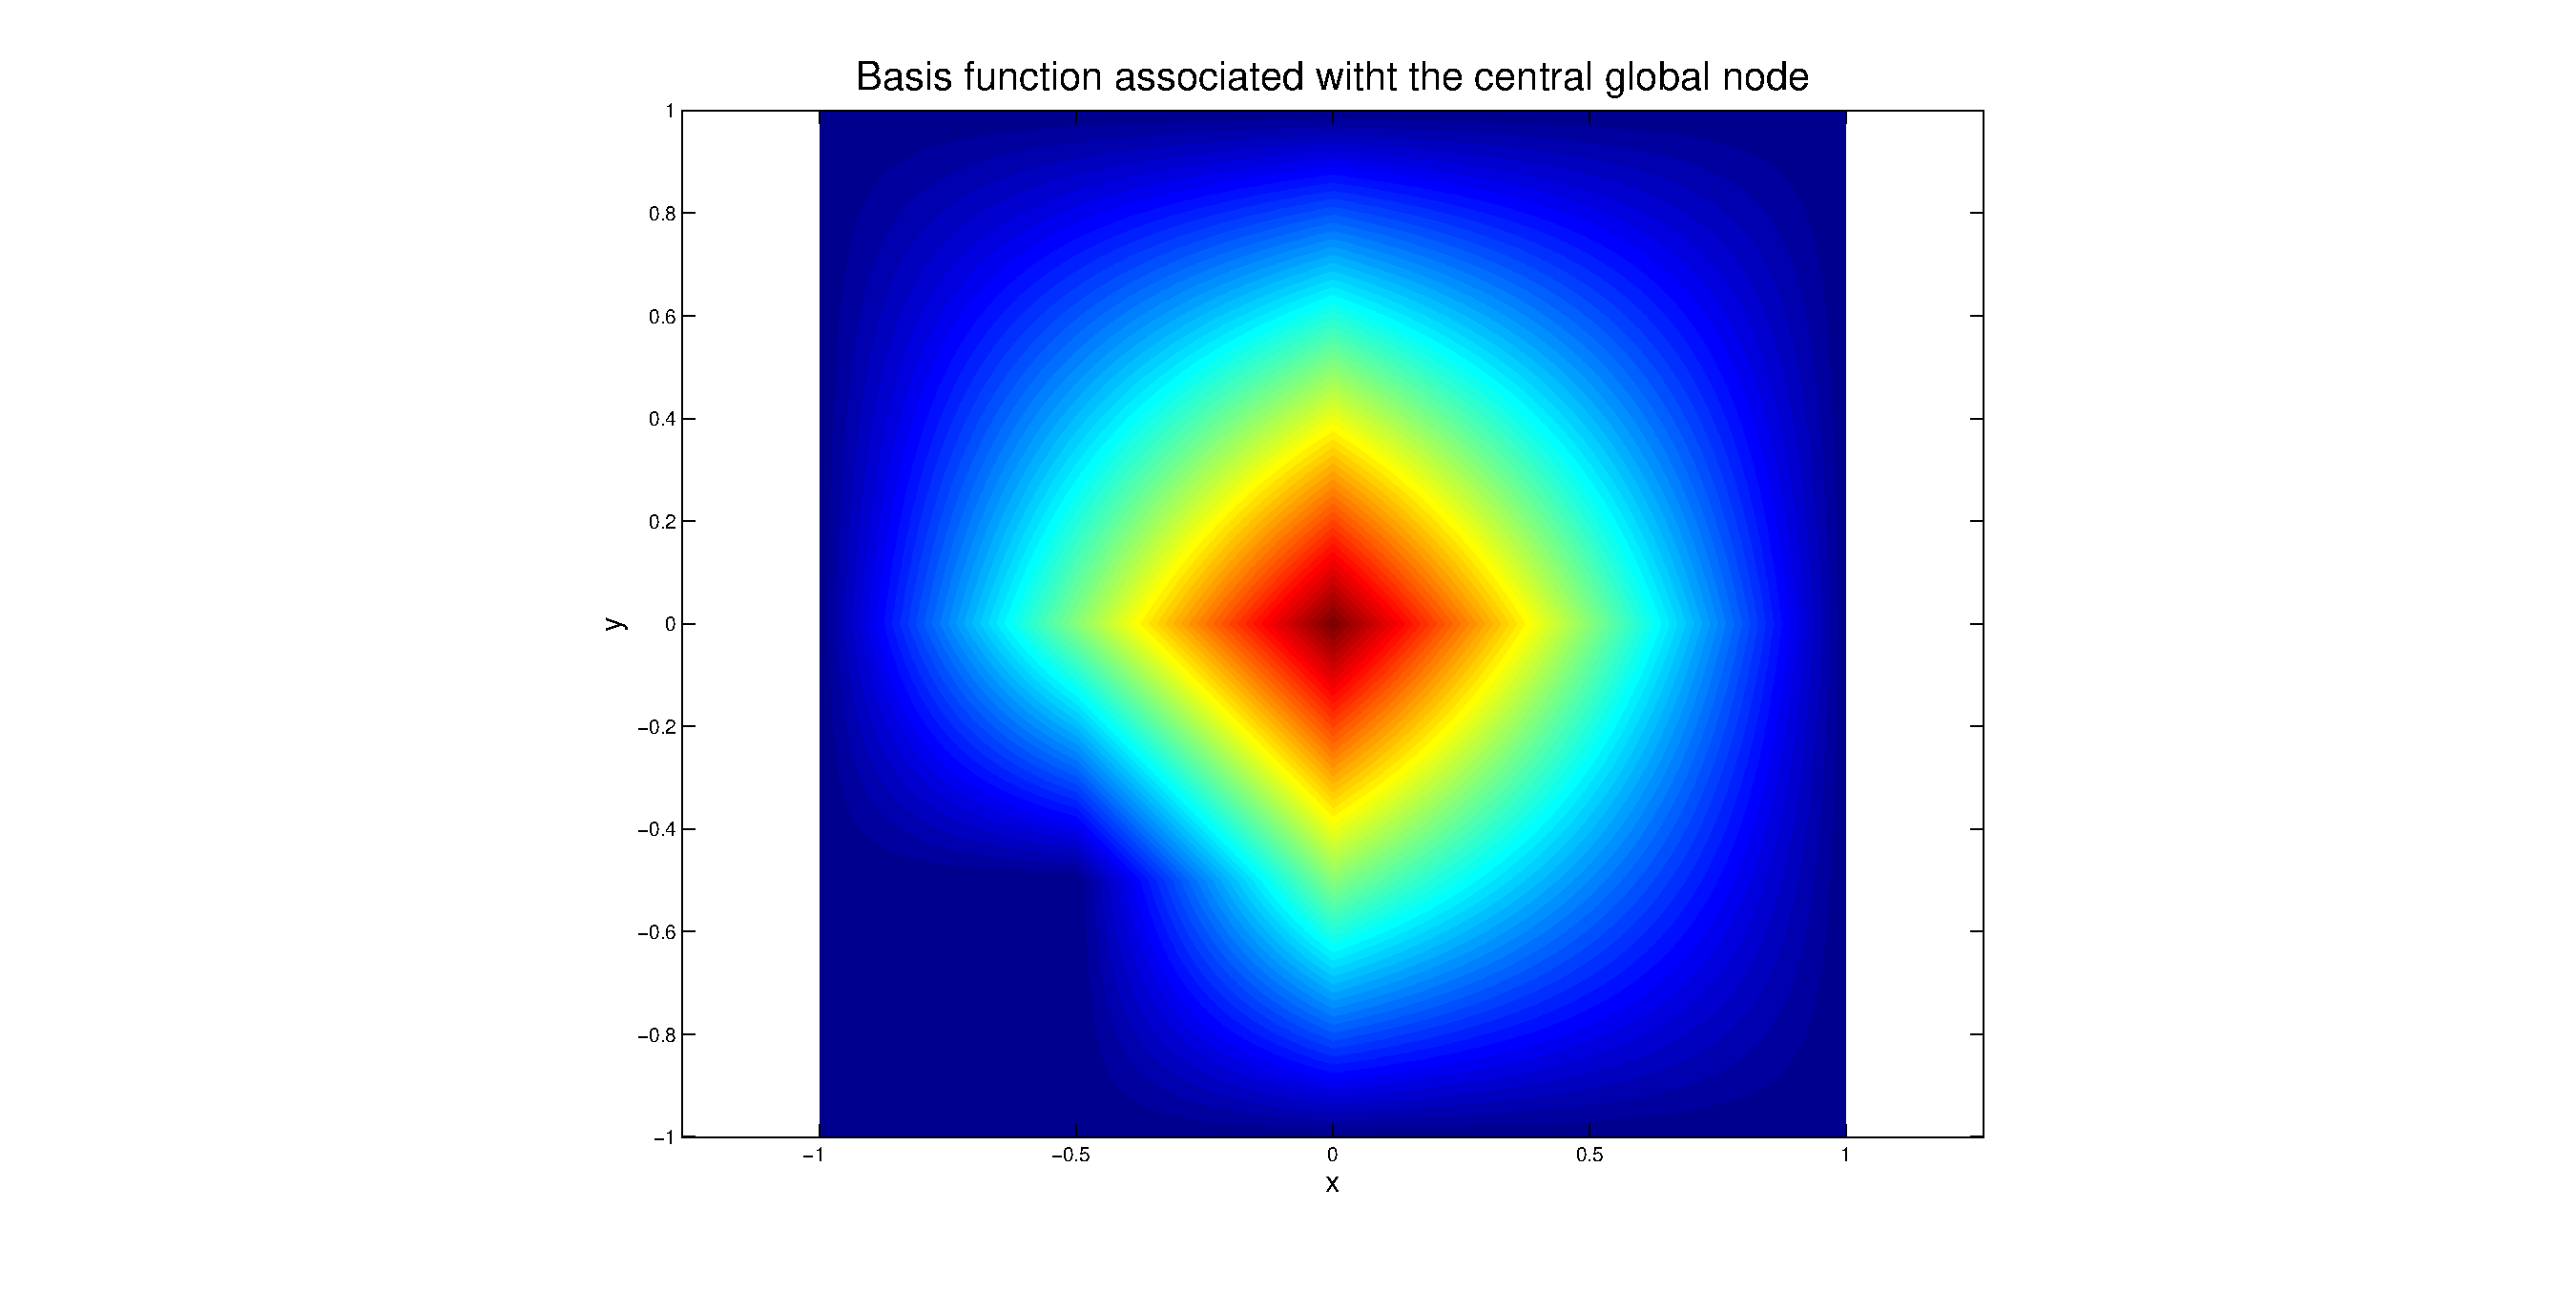
\includegraphics[scale=0.35]{Theory/global_basis_func.eps}
\caption{Global basis function associated with the global GLL node located in the center of the mesh presented in figure \ref{hang_ex} for $p=1$.}
\label{global_basis_func}
\end{figure}


Figure \ref{global_basis_func} shows a global basis function on the mesh presented in figure \ref{hang_ex} for $p=1$. We can see that it is not entirely trivial since the global node associated with the basis function has a influence in quadrants where we have hanging nodes. We can also see that it is indeed a continuous function that is a piece-wise bilinear polynomial. 

Let us also note that there is no global basis function associated with a hanging node. 

In practice, we do not build the operator $R^e_{ij}(I)$ explicitly since only nodes located on edges can be hanging and the p4est library helps us to treat hanging nodes (see the implementation chapter for more details).  

\subsection{Computing the right-hand side}

Now that we have defined our global basis functions, it is possible to perform the integration needed to compute $b_j$ (equation \ref{eq:b}). As explained before, we will perform the integration quadrant by quadrant. Let us denote : 

$$ b_I^e = -\int_{\Omega_e} f\phi_I\:dxdy$$

We obviously have that $b_I = \sum_e b_I^e$. Let us also define the reference element associated with quadrant $e$ by $\hat{\Omega}_e$ and the jacobian of the mapping as : 

$$ J^e (\xi,\eta) = \begin{pmatrix}
\frac{\partial x^e}{\partial \xi} & \frac{\partial x^e}{\partial \eta}\\
\frac{\partial y^e}{\partial \xi} & \frac{\partial y^e}{\partial \eta}
\end{pmatrix}$$

Then the integration on quadrant $e$ becomes : 

$$b_I^e = -\int_{\hat{\Omega}_e} f(x^e(\xi,\eta),y^e(\xi,\eta)) \phi_I(x^e(\xi,\eta),y^e(\xi,\eta)) |J^e(\xi,\eta)| \: d\xi d\eta$$

Using equation \ref{eq:global_basis}, we get : 

$$b_I^e = -\int_{\hat{\Omega}_e} f(x^e(\xi,\eta),y^e(\xi,\eta)) \left( \sum_{i=0}^p\sum_{j=0}^p R^e_{ij}(I) l_i(\xi)l_j(\eta) \right) |J^e(\xi,\eta)| \: d\xi d\eta $$

This is where the fact that our global nodes are also GLL nodes becomes important. To alleviate a little the formulas, let us define two new notations :  $J^e(\xi_m,\eta_n) = J^e_{mn}$ and $f(x^e(\xi_m,\eta_n),y^e(\xi_m,\eta_n)) = f^e_{mn}$. Using the GLL quadrature rule, we have : 

$$ b_I^e = - \sum_{m=0}^p\sum_{n=0}^p w_m w_n f^e_{mn} \left( \sum_{i=0}^p\sum_{j=0}^p R^e_{ij}(I) l_i(\xi_m)l_j(\eta_n) \right) |J^e_{mn}|$$

Since $l_i(\xi_j) = \delta_{ij}$, this becomes : 

$$  b_I^e = - \sum_{m=0}^p\sum_{n=0}^p w_m w_n f^e_{mn} R^e_{mn}(I) |J^e_{mn}|$$

This expression looks more complicated than it actually is. Indeed, the operator $R_{mn}^e(I)$ is often equal to zero. It is non zero only if in quadrant $e$, the local node $(m,n)$ is the global node $I$ (in which case it is equal to 1) or if the local node $(m,n)$ is located on a hanging edge where the global node $I$ has an influence. Therefore, in a quadrant where we do not have hanging nodes, and if the local node $(m,n)$ has $I$ as global number, we simply have : 

$$b_I^e = - w_m w_n f^e_{mn} |J^e_{mn}|$$

\subsection{Computing a matrix-vector product}

As said in the introduction, we will use an iterative method to solve the system presented by equations \ref{eq:A} and \ref{eq:b}, namely the preconditioned conjugate gradients. As a result, we do not need to build the matrix $A$ explicitly but rather we need to be able to perform a matrix-vector product $Au$ where $u$ is a vector containing the values of our numerical solution at the global nodes, i.e. $u_I$ is the value of the solution at global node $I$. By linearity of the integral and the derivative, and the definition of $u^h$, we have : 

\begin{align*}
(Au)_I =& \sum_{J=1}^N \int_\Omega \nabla \phi_I \cdot \nabla \phi_J \:dxdy \: u_J\\
=& \int_\Omega \nabla \phi_I \cdot \nabla\left(\sum_{J=1}^N \phi_Ju_J\right)\:dxdy\\
=& \int_\Omega \nabla \phi_I \cdot \nabla u^h \: dxdy
\end{align*}

Just as in the previous subsection, we will compute this integral quadrant by quadrant. The first thing we want to do is to compute the value of $u^h$ at the local GLL nodes on quadrant $e$. Let us define, $u^e_{mn}$ as this local value : 

$$u^e_{mn} = \sum_{I=1}^N R_{mn}^e(I) u_I$$

Let us then define $u^e$ as the restriction of $u^h$ on quadrant $e$. Since we know that, on quadrant $e$, $u^h$ must be a polynomial of degree $p$ going through the $(p+1)^2$ GLL local nodes whose values are given by $u_{mn}^e$ for $m,n=0,...,p$, and since we know that such a polynomial is unique, we have : 

\begin{align*}
u^e(x,y) &= \sum_{m=0}^p \sum_{n=0}^p u^e_{mn}l_m(\xi^e(x,y))l_n(\eta^e(x,y)) &\text{if $(x,y)\in \Omega_e$}
\end{align*}

Using our restriction, the linearity of the different operators and the equation \ref{eq:global_basis}, we have :  

\begin{align}
(Au)_I^e =& \int_{\Omega_e} \nabla \phi_I \cdot \nabla u^h\: dxdy \nonumber\\
=& \int_{\Omega_e} \nabla \phi_I \cdot \nabla u^e\: dxdy \nonumber\\
=& \sum_{m=0}^p\sum_{n=0}^p R^e_{mn}(I) \int_{\Omega_e} \nabla \left( l_m(\xi^e(x,y))l_n(\eta^e(x,y)\right) \cdot \nabla u^e \: dxdy \label{eq:Au_last}
\end{align}

Let us now focus on the last part of equation \ref{eq:Au_last}. Since we want to integrate on the reference element, we first have to take care of the derivatives. To simplify the notations, let us define : $L_{mn}(\xi,\eta) = l_m(\xi)l_n(\eta)$. Then, using the chain rule, we have : 

\begin{align*}
\int_{\Omega_e} \nabla \left( l_m(\xi^e(x,y))l_n(\eta^e(x,y)\right) \cdot \nabla u^e \: dxdy = &\int_{\hat{\Omega}_e} \left(\frac{\partial L_{mn}}{\partial\xi}\frac{\partial\xi}{\partial x}+\frac{\partial L_{mn}}{\partial\eta}\frac{\partial\eta}{\partial x}\right)\left(\frac{\partial u^e}{\partial\xi}\frac{\partial\xi}{\partial x}+\frac{u^e}{\partial\eta}\frac{\partial\eta}{\partial x}\right) |J^e|\\
&+  \left(\frac{\partial L_{mn}}{\partial\xi}\frac{\partial\xi}{\partial y}+\frac{\partial L_{mn}}{\partial\eta}\frac{\partial\eta}{\partial y}\right)\left(\frac{\partial u^e}{\partial\xi}\frac{\partial\xi}{\partial y}+\frac{u^e}{\partial\eta}\frac{\partial\eta}{\partial y}\right)|J^e| \: d\xi d\eta 
\end{align*}

It is then a matter of rearranging the different terms. 

\begin{align*}
\int_{\Omega_e} \nabla \left( l_m(\xi^e(x,y))l_n(\eta^e(x,y)\right) \cdot \nabla u^e \: dxdy &= F^{\xi\xi}_{mn;e} + F^{\xi\eta}_{mn;e} + F^{\eta\xi}_{mn;e} + F^{\eta\eta}_{mn;e} \\
F^{\xi\xi}_{mn;e} &= \int_{\hat{\Omega}_e} \frac{\partial L_{mn}}{\partial \xi}\frac{\partial u^e}{\partial \xi} \left(\frac{\partial \xi}{\partial x}\frac{\partial \xi}{\partial x}+\frac{\partial \xi}{\partial y}\frac{\partial \xi}{\partial y}\right) |J^e| d\xi d\eta\\
F^{\xi\eta}_{mn;e} &= \int_{\hat{\Omega}_e} \frac{\partial L_{mn}}{\partial \xi}\frac{\partial u^e}{\partial \eta} \left(\frac{\partial \xi}{\partial x}\frac{\partial \eta}{\partial x}+\frac{\partial \xi}{\partial y}\frac{\partial \eta}{\partial y}\right) |J^e| d\xi d\eta\\
F^{\eta\xi}_{mn;e} &= \int_{\hat{\Omega}_e} \frac{\partial L_{mn}}{\partial \eta}\frac{\partial u^e}{\partial \xi} \left(\frac{\partial \eta}{\partial x}\frac{\partial \xi}{\partial x}+\frac{\partial \eta}{\partial y}\frac{\partial \xi}{\partial y}\right) |J^e| d\xi d\eta\\
F^{\eta\eta}_{mn;e} &= \int_{\hat{\Omega}_e} \frac{\partial L_{mn}}{\partial \eta}\frac{\partial u^e}{\partial \eta} \left(\frac{\partial \eta}{\partial x}\frac{\partial \eta}{\partial x}+\frac{\partial \eta}{\partial y}\frac{\partial \eta}{\partial y}\right) |J^e| d\xi d\eta
\end{align*}

We will again use the GLL quadrature to compute those integrals. Once again, the fact that the quadrature nodes are the same as our local nodes will allow us to compute the different terms efficiently. Let us introduce a few definitions : 

\begin{align*}
W_{ij;e}^{\xi\xi} =& w_i w_j |J^e(\xi_i,\eta_j)| \left(\frac{\partial \xi}{\partial x}\frac{\partial \xi}{\partial x}+\frac{\partial \xi}{\partial y}\frac{\partial \xi}{\partial y}\right)(\xi_i,\eta_j)\\
W_{ij;e}^{\xi\eta} =& w_i w_j |J^e(\xi_i,\eta_j)| \left(\frac{\partial \xi}{\partial x}\frac{\partial \eta}{\partial x}+\frac{\partial \xi}{\partial y}\frac{\partial \eta}{\partial y}\right)(\xi_i,\eta_j)\\
W_{ij;e}^{\eta\eta} =& w_i w_j |J^e(\xi_i,\eta_j)| \left(\frac{\partial \eta}{\partial x}\frac{\partial \eta}{\partial x}+\frac{\partial \eta}{\partial y}\frac{\partial \eta}{\partial y}\right)(\xi_i,\eta_j)
\end{align*}

The derivatives that appear in the expression above do not need an analytic expression for the inverse mapping to be available. We can compute them using the inverse of the jacobian matrix to obtain the values of $\frac{\partial xi}{\partial x}(\xi_i,\eta_j)$,...

Let us also remind the definition of the derivation matrix $H$ given by equation \ref{eq:derivation_matrix}. Using the quadrature, we have : 

\begin{align*}
F^{\xi\xi}_{mn;e} =& \sum_{a=0}^p\sum_{b=0}^p W^{\xi\xi}_{ab;e} l'_m(\xi_a)l_n(\eta_b)\left( \sum_{c=0}^p\sum_{d=0}^p u^e_{cd}l'_c(\xi_a)l_d(\eta_b)\right) \\
=& \sum_{a=0}^p\sum_{b=0}^p W^{\xi\xi}_{ab;e} H_{ma} \delta_{nb} \left( \sum_{c=0}^p\sum_{d=0}^p u^e_{cd}H_{ca}\delta_{db}\right) \\
=& \sum_{a=0}^p W_{an;e}^{\xi\xi}H_{ma}\left(\sum_{c=0}^p u^e_{cn}H_{ca}\right)
\end{align*}

If we denote $U^e$ a matrix such that $(U^e)_{ij} = u^e_{ij}$ and $W^{\xi\xi}_e$ a matrix such that $(W^{\xi\xi}_e)_{ij} = W^{\xi\xi}_{ij;e}$ and if we denote the Hadamard product by $\circ$,  then we can write : 

\begin{align*}
F^{\xi\xi}_{mn;e} &= \left( H(W_e^{\xi\xi} \circ H^TU^e)\right)_{mn}
\end{align*}

For similar definitions, it can be showed that the order terms are given by :  

\begin{align*}
F^{\xi\eta}_{mn;e} &= \left( H(W_e^{\xi\eta} \circ U^eH)\right)_{mn}\\
F^{\eta\xi}_{mn;e} &= \left( (W_e^{\eta\xi} \circ H^TU^e)H^T\right)_{mn}\\
F^{\eta\eta}_{mn;e} &= \left( (W_e^{\eta\eta} \circ U^eH)H^T\right)_{mn}
\end{align*}

We can see that the problem reduce to computing a few matrix products. The only thing left to do is to take hanging nodes into account when we gather the results : 

\begin{align*}
(Au)^e_I &= \sum_{m=0}^p\sum_{n=0}^p R^e_{mn}(I) \left(F_{mn;e}^{\xi\xi}+F_{mn;e}^{\xi\eta}+F_{mn;e}^{\eta\xi}+F_{mn;e}^{\eta\eta} \right)
\end{align*}

And, of course, we need to take the influence of every quadrant into account : 

\begin{align*}
(Au)_I &= \sum_e (Au)_I^e
\end{align*}




\section{Preconditioned conjugate gradients}

Now that we have our right hand side vector $b$ and that we are able to compute a matrix-vector product $Au$, we can explain how to solve the linear system. 

Since the number of degrees of freedom is huge, it is impossible to use a direct method to solve the linear system. Instead, we will turn ourselves to iterative methods. 

The matrix $A$ arises from the discretization of an Poisson equation using finite elements and therefore it is sparse, symmetric and positive-definite (see \textcolor{red}{ref here}). The conjugate gradients method is therefore well suited to solve the linear system. We have to note however that the convergence speed of the conjugate gradients depends on the condition number of the matrix $A$, $\kappa(A)$. Indeed, as given in \textcolor{red}{ref here}, if we denote $e_i = u-u_i$ where u is the solution of the linear system and $u_i$ is our approximation after the $i$-th iteration, then : 

\begin{align}
||e_i||_A \leq 2 \left(\frac{\sqrt{\kappa(A)}-1}{\sqrt{\kappa(A)}+1}\right)^i ||e_0||_A \label{eq:cg_conv}
\end{align}


Where $||e_i||_A = \left(e_i^TAe_i\right)^\frac{1}{2}$. We can see in equation \ref{eq:cg_conv} that the higher the condition number of $A$, the slower the convergence.  

Unfortunately, the condition number of the matrix $A$ is often very large and that is why we need to use a preconditioner. 

Formally, we want to solve : 

$$Au=b$$

Which is equivalent to solving : 

$$M^{-1}A u = M^{-1}b$$

If $M$ is easy to invert and $\kappa(M^{-1}A) \ll \kappa(A)$, then we should have a faster convergence at not too great a cost. The problem is that it is not possible to guarantee that $M^{-1}A$ is either symmetric nor positive definite, which is required for the CG.

However, we know that if $M$ is symmetric and positive-definite, then there exists a matrix $E$ such that $M = EE^T$. We can also note that $M^{-1}A$ and $E^{-1}AE^{-T}$ have the same eigenvalues. Indeed, let us assume that $v$ if an eigenvector of $M^{-1}A$ associated with eigenvalue $\lambda$. Then :

$$E^{-1}AE^{-T} (E^{T}v) = (E^{T}E^{-T})E^{-1}Av = E^{T}M^{-1}Av = \lambda E^Tv$$

And we can conclude that $E^Tv$ is an eigenvector of $E^{-1}AE^T$ with eigenvalue $\lambda$. If the two matrices have the same eigenvalues, they also have the same condition number. If $A$ is symmetric and positive-definite, it is clear that $E^{-1}AE^{-T}$ is also symmetric and positive-definite. We can thus use the CG to solve the following system (which is equivalent to $Au=b$) : 

\begin{align*}
E^{-1}AE^{-T} \hat{u} &= E^{-1}b &\hat{u} = E^{T}u
\end{align*}

This formulation has the unwanted property of making explicit use of the matrix $E$. We would like to remove it entirely and use $M$ only. It is indeed possible (see \textcolor{red}{ref here}).

Let us define $u_i$ the approximation after the $i$-th approximation and $r_i = b-Au_i$. Then, the PCG procedure is given by algorithm \ref{pcg}. We can note that we indeed do not mention $E$ but use $M^{-1}$ instead. We can also see that we start with a zero initial guess. It does not have to be the case and if we had a better initial guess, we should use it. 

\begin{algorithm}
\begin{algorithmic}
\State $u_0 = 0$
\State $r_0 = b-Au_0$
\State $z_0 = M^{-1}r_0$
\State $p_0 = z_0$
\State $i = 0$
\While{$||r_i||_2 > \epsilon ||r_0||_2$}
\State $d_i = Ap_i$
\State $\alpha_i = \frac{r_i^Tz_i}{p^T_id_i}$
\State $u_{i+1} = u_i + \alpha_i p_i$
\State $r_{i+1} = r_i - \alpha_i d_i$
\State $z_{i+1} = M^{-1}r_{i+1}$
\State $\beta_{i+1} = \frac{z_{i+1}^Tr_{i+1}}{z_i^Tr_i}$
\State $ p_{i+1} = z_{i+1} + \beta_{i+1}p_i$
\State $i = i+1$
\EndWhile
\end{algorithmic}
\caption{Preconditioned Conjugate Gradients}
\label{pcg}
\end{algorithm}

The stopping criterion is defined using the norm of the residual. We want it to be less than a given fraction of the norm of the initial residual. 

The most important part in the algorithm presented is the preconditioner $M^{-1}$. Indeed, the convergence speed is a function of $\kappa(M^{-1}A)$. Therefore, we want a preconditioner that is easy to compute and such that the condition number of $M^{-1}A$ is a lot smaller than the one of $A$. Oftentimes, those two goals are contradictory. 

As explained in the introduction, our preconditioner here consists of two parts. We have one coarse grid correction based on solving the problem on the mesh with an interpolation of degree $p=1$. The resolution of this coarse problem will be done using a multigrid method. Let us call this part $P^c$. The second part is the fine preconditioner where we solve the problem exactly on overlapping subdomains (this is often called an additive Schwarz preconditioner). Let us call this part $P^f$. We then add the two part of the preconditioner : 

$$ M^{-1} = P^c + P^f$$

The hope is that the two parts of the preconditioner act on different parts of the problem and that the sum of the two makes a good preconditioner. The rest of this chapter is entirely about how to compute $M^{-1}r = P^cr+P^fr$.

 


\section{Coarse preconditioner : the multigrid solver}

Let us first present the coarse part of the preconditioner. It consists of solving the problem on the mesh using an interpolation of degree $p=1$ with a geometric multigrid method. 

Since in general we use an interpolation degree $p$, the first thing to do is to restrict this residual on the same mesh but for a degree $p=1$. The first part of this section presents the restriction used. Similarly, once we have computed the solution for $p=1$, we have to prolong it to a higher degree. To preserve the symmetry of the problem, we will define the prolongation operator to be the transpose of the restriction operator. The procedure explained here is an application with hanging nodes of the one described in \cite{remacle}. Formally, if we denote by $S$ the restriction operator and by $G$ the geometric multigrid solver, we have : 

$$P^cr = S^TGSr$$

The second part explains in more details what are the key components of the geometric multigrid solver. The practical implementation and the way it works with p4est is however described in the next chapter. 

We have to note that the coarse preconditioner cannot be use as the only preconditioner for the CG. Indeed, because of the restriction, it has a kernel, i.e. it is possible to have a high degree residual $r\neq 0$ such that : 

$$Sr = 0$$

As a result, the PCG will stop even tough we have not reached the solution. That is why, in the results chapter, we never test the multigrid alone with a degree superior to $p=1$. 

\subsection{Restriction of $r$ from a high degree to $p=1$}

Let us now define the operator $S$ that will restrict the high degree residual $r$ to a low degree $p=1$. Authors of \cite{l2proj} have shown that a good choice for the restriction is the $L^2$ projection. 

Let us call $V^h_p \subset H^1(\Omega)$ the space whose basis consists of the high degree global basis functions (later denoted $\phi_i$ for $i=1,...,N$) and $V^h_1 \subset H^1(\Omega)$ the one whose basis is constituted by the bilinear global basis function (later denoted $\Phi_i$ for $i=1,...,M$). We want to find $R \in V^h_1(\Omega)$ such that $R$ is the $L^2$ projection of $r \in V^p(\Omega)$ onto $ V^h_1(\Omega)$. As shown in \cite{remacle}, the $L^2$ projection is then given by :

$$ R = Cm^{-1}r$$ 

Where $m$ is the high degree mass matrix and $C$ is called the correlation matrix. The mass matrix $m$ is easy to invert since in the case of spectral elements, it is diagonal, i.e. we have :

\begin{align*}
m_{ij} &= \int_\Omega \phi_i\phi_j \: dxdy \approx 0  &\text{if $i\neq j$}
\end{align*}

%\begin{align*}
%\int_\Omega \phi_i\phi_j \:dxdy &= \sum_{e} \int_{\Omega_e} \phi_i\phi_j \:dxdxy\%\
%&=  \sum_{e} \int_{\Omega_e} \left(\sum_{a=0}^p\sum_{b=0}^p R^e_{ab}(i)l_al_b%\right) \left( \sum_{c=0}^p\sum_{d=0}^p R^e_{cd}(j)l_cl_d\right) \: dxdy\\
%&\approx \sum_e \sum_{m=0}^p\sum_{n=0}^p w_mw_n |J^e_{mn}| %\left(\sum_{a=0}^p\sum_{b=0}^p R^e_{ab}(i)\delta_{am}\delta_{bn}\right) \left( %\sum_{c=0}^p\sum_{d=0}^p R^e_{cd}(j)\delta_{cm}\delta_{dn}\right)\\
%&= \sum_e \sum_{m=0}^p\sum_{n=0}^p w_mw_n |J^e_{mn}|  R_{mn}^e(i)R_{mn}%^e(j)
%\end{align*}

The other term is the correlation matrix. It is defined by : 

$$ C_{I,i} = \int_\Omega \Phi_I\phi_i \: dxdy$$

We can also define its local counterpart using local shape functions. Let us denote $l_i$ the one dimensional shape function of degree $p$ associated with the $i$-th GLL node and $L_i$ the one dimensional linear shape function associated with the $i$-th GLL node. Then we have :

$$ C_{IJ,ij;e} = \int_{\Omega_e} L_IL_J l_il_j \: dxdy$$

If we use the GLL quadrature using the $(p+1)^2$ GLL nodes on quadrant $e$, we get : 

$$C_{IJ,ij;e} \approx w_iw_j|J^e_{ij}| \Phi_I(\xi_i)\Phi_J(\xi_j)$$

For later purposes, let us define : 

\begin{align*}
m_{ij;e} &= w_iw_j|J^e{ij}|\\
B_{IJ,ij} &= \Phi_I(\xi_i)\Phi_J(\xi_j)
\end{align*}

We can then compute the restriction of $r$ as : 

\begin{align*}
y &= m^{-1}r\\
R &= Cy
\end{align*}

Applying $m^{-1}$ to $r$ is rather easy : we only scale the residual by the inverted mass matrix. We now have to transfer $y_i$ for $i=1,...,N$ onto each local quadrant $e$. For this, let us use the operator $R^e_{ij}$ to handle hanging nodes : 

$$ y_{ij;e} = \sum_{K=1}^N R^e_{ij}(K) y_K$$

Let us then compute the local coarse grid residual using the correlation matrix in its local form. This yields :

$$R_{IJ;e} = \sum_{i=0}^p\sum_{j=0}^p B_{IJ,ij}m_{ij;e}y_{ij;e}$$

The last remaining thing to do is to gather the local coarse grid residual to obtain the global coarse grid residual. Let us do not forget to handle the hanging nodes and therefore to use the operator $R^e_{IJ}$ (not to confuse with $R_{IJ;e}$ the local coarse grid residual on quadrant $e$). Let us note that it is not the same as $R^e_{ij}$ since it works on the global nodes for bilinear interpolation where $R^e_{ij}$ is used for the interpolation of degree $p$. 

$$ R_K = \sum_e \sum_{I=0}^1\sum_{J=0}^1 R^e_{IJ}(K) R_{IJ;e}$$

This residual $R$ is then used as a right-hand side for the multigrid solver. 

\subsection{Prolongation of the solution from $p=1$ to a high degree}

Let us assume that the solution given by the multigrid solver with $R$ as right-hand side is given by $Z$, i.e. : 

$$ Z = GR$$

We now need to prolong this coarse scale correction onto the fine grid. Since the prolongation operator is defined as the transpose of the restriction operator, we have : 

$$P^cr = m^{-1}C^TZ$$

The global coarse correction $Z$ is first scattered to each element to have the local coarse scale correction. Let us not forget to handle hanging nodes : 

$$Z_{IJ;e} = \sum_{K=1}^M R_{IJ}^e(K) Z_K$$

Then, let us prolong the correction to obtain :

$$z_{ij;e} = \sum_{I=0}^1\sum_{J=0}^1 B_{IJ,ij}m_{ij;e}Z_{IJ;e}$$

We then have to gather $z_{ij;e}$ to compute its global counterpart. Once again, this is where we handle hanging nodes.

$$z_{K} = \sum_e\sum_{i=0}^p\sum_{j=0}^p R^e_{ij}(K)z_{ij;e}$$

The last thing left to do is to scale $z_K$ by the inverted mass matrix. This yields : 

$$(P^cr)_K = \frac{z_K}{m_K}$$

\subsection{The geometric multigrid solver}

This subsection generally describe how the geometric multigrid method works and why it is so effective. However, a lot of details have been omitted and more information can be obtained in the relevant literature (for example in \cite{multi_book}). It has to be noted that here the degree of interpolation is always $p=1$.

\subsubsection{Motivation}

The first observation we have to make is that for any known function $v$ such that $v(x,y)=u_0$ if $(x,y) \in \Gamma$, we can rewrite problem \ref{eq:poisson}. Indeed, if we define a function $e = u-v$, then we have

\begin{align}
\nabla ^2 e &= f-\nabla^2v = r &\text{on $\Omega$} \label{eq:poisson_error}\\
e &= u-v = 0 &\text{on $\Gamma$}
\end{align}

Which is qualitatively the same problem. But if we are able to solve it for $e$ more easily than we would have been able to do it for $u$, then we can simply recover $u$ from $e$ : 

$$u = v + e$$

The second observation we have to make is that the discretization of problem \ref{eq:poisson} or equivalently the one above yields a linear system of equations to solve (as the one derived in the first section of this chapter). As already mentioned, the matrix $A$ defining this linear system has very often a very large condition number $\kappa(A)$. As a result, using iterative methods can be very slow. Typically, the condition number of $A$ for $p=1$ is $\mathcal{O}(h^2)$ where $h$ is the size of the smallest quadrant (see \cite{condNumb}). Thus, if we use a coarser grid (where the smallest quadrant has a larger size than before), the problem is easier to solve. 

The idea behind multigrid is therefore a two-level idea. It works as follow : 

\begin{enumerate}
\item Given an approximate solution to the problem, compute the residual $f-\nabla^2v$.
\item Solve problem \ref{eq:poisson_error} to obtain $e$. It should be easier to solve than the initial problem by using a coarser grid.
\item Add $e$ to $v$ to get the solution $u$. 
\end{enumerate}

The next step in the reasoning is to use this idea recursively. Indeed, in step 2, to solve problem \ref{eq:poisson_error}, one can reuse the same process. A more precise definition of the algorithm is given at the end of this section, in algorithms  \ref{mu_cycle} and \ref{multi_algo}.

We still have not explained two things in the procedure above. The first is how to choose an approximate solution to the problem. In theory, it can be any but we have to remember that, in step 2, we will use a coarser grid to solve for $e$. As a result, we want an approximation such that $e = u-v$ is a smooth function that a coarse grid can capture well. One way to obtain this approximation is by using an iterative method. Indeed, it has been shown (for example, in \cite{smoothing}) that even tough iterative methods like Jacobi or Gauss-Seidel have a tendency to stall, just a few iterations allows them to capture the high-frequency modes in the solution. That means that if we compute $v$ by doing some iterations of the Jacobi method, then $e = u-v$ will contain only low frequency modes. And a solution containing low frequencies can be computed on a coarser grid. This property that the high frequency errors converge a lot quicker than the low frequency error is called the smoothing property and is hold by a lot of different smoother (for example, the Jacobi method).

The second thing we have to consider is how to transfer one function onto another grid. Indeed, in step 1, we compute the residual $f-\nabla^2 v$ but then we have to solve problem \ref{eq:poisson_error} on a different, coarser grid. We therefore need an operator to compute the right-hand side of the linear system on the coarser grid from the right-hand side of the one on the initial grid. This is called the restriction operator. Similarly, when we have computed the solution on the coarser grid in step 2, we need to update our approximation $v$ with $e$ on the initial grid. This operator is called the prolongation operator. We will see that there exists a link between those two operators.

\subsubsection{The smoother : damped Jacobi method}

Let us now present the smoother used : the damped Jacobi method. Let us assume that we want to solve :

$$Av=b$$

Let us then split the matrix $A$ in the form : 

$$(D-L-U)v = b$$

Where $D$ is a diagonal matrix containing the diagonal of $A$, $-L$ is the strictly lower triangular part and $-U$ is the strictly upper triangular part. Let us also denote as $v^i$ the approximation of the solution of $Av=b$ after the $i$-th iteration. Then, the damped Jacobi method with damping factor $\omega$ is given by : 

$$ v^{i+1} = \omega\left(D^{-1}(L+U)v^i + D^{-1}b\right) + (1-\omega)v^i$$

It is to be noted that since $D$ is diagonal, it is very cheap to compute $D^{-1}$. It can be shown (see \cite{multi_book}) that if $0<\omega\leq 1$ then the damped Jacobi method is stable. The parameter $\omega$ can then be tuned to obtain different properties in the convergence of high frequency errors. In \cite{multi_book}, it is shown that a good choice for $\omega$ is : 

$$\omega = \frac{2}{3}$$

We now have to explain how to compute $A$ for the different grids. Since it results from the discretization of problem \ref{eq:poisson_error}, we can use the same method as the one explained in the section concerning the spectral element method. It is here even easier since we have piece-wise bilinear global basis function. We however still have to be careful of hanging nodes. The next chapter explains in more details the implementation. 

\subsubsection{Prolongation operator}

Let us now define the prolongation operator, i.e. the operator that takes the solution to problem \ref{eq:poisson_error} on the coarse grid and prolong it on the fine grid. 

\begin{figure}
\centering
\begin{subfigure}{.5\textwidth}
  \centering
  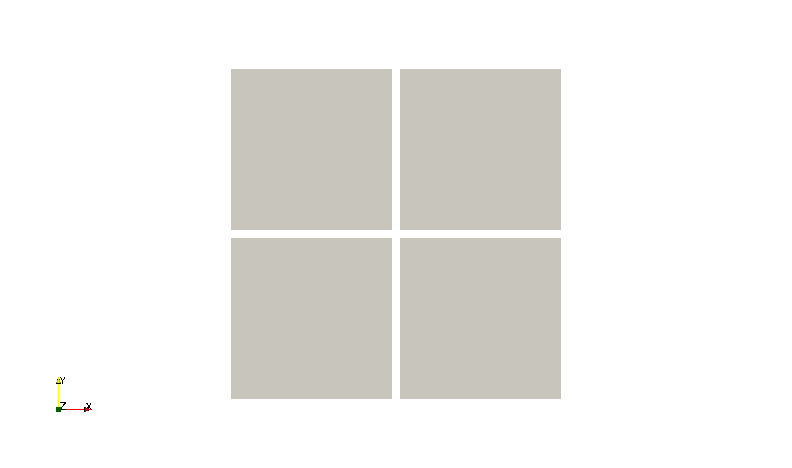
\includegraphics[width=1.2\linewidth]{Theory/hang_lev_1.png}
  \caption{Mesh at level 1}
  \label{hang_lev_1}
\end{subfigure}%
\begin{subfigure}{.5\textwidth}
  \centering
  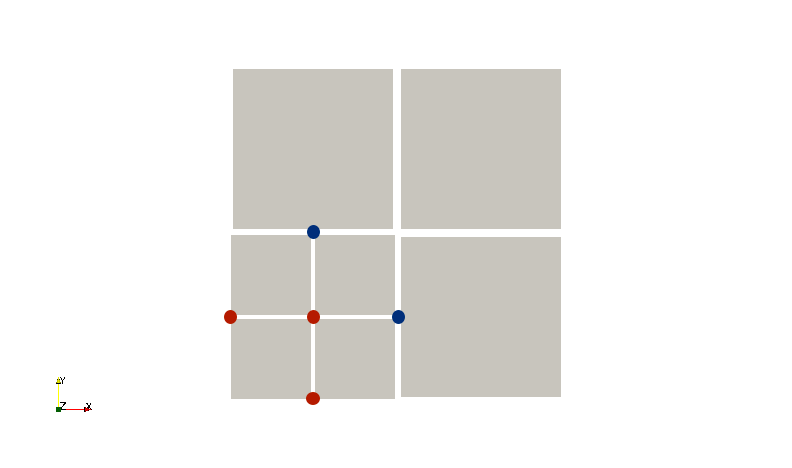
\includegraphics[width=1.2\linewidth]{Theory/hang_lev_2.png}
  \caption{Mesh at level 2}
  \label{hang_lev_2}
\end{subfigure}
\caption{Example of two meshes used in the geometric multigrid method. The one on the left is the coarser mesh, where all quadrants have a refinement level of 1. The one on the right has some quadrants that have a level of refinement of 2 and is therefore the level 2 mesh. We can also see the influence of increasing by one level. We have the apparition of three new global nodes (in red) and two new hanging nodes (in blue).}
\label{hang_lev}
\end{figure}

In order to do this, we have to precise the nature of the different meshes that will be used. As explained earlier, we will solve the problem on different meshes. Let us organize those meshes on different levels, where the lowest level has the coarsest mesh and the highest level has the finest mesh.  The AMR provides us with a natural choice for the definition of those meshes. Indeed, since each quadrant is dynamically refined, we will consider the mesh at level $lev$ to be the original mesh where the maximum level of refinement is $lev$ (see for example \cite{levelMulti}). An example is given on figure \ref{hang_lev}. We can see that the mesh on the left has all its quadrants with a refinement level of 1, it is thus the mesh at level 1. On the right, the mesh has some (but not all) quadrants that have a refinement level of 2. It is therefore the mesh at level 2. 

Now that we have some sense of how the meshes are constructed, it is possible to define the prolongation operator. We can see on figure \ref{hang_lev_2} the influence of increasing by one level. There is the apparition of three new global nodes (in red) and two new hanging nodes (in blue).

Since we use a bilinear interpolation (thus linear along each edge), the prolongation operator is quite natural : the new node created in the middle of a refined quadrant (and that can never be hanging) is equal to a fourth of the sum of the values at the corners of the larger quadrant. Concerning the nodes added on the edges, if they are not hanging, they are equal to half of the sum of the values at the ends of the edge. Of course, we do not need to compute the prolongation for the hanging edges since they are not global. 

\subsubsection{Restriction operator}

As before, to conserve the symmetry of the problem, the restriction operator is defined as the transpose of the prolongation operator. 

It means that if a group of four quadrants has to be coarsened to move to the mesh a level below, the value of the residual at the middle node (once again, it can never be hanging) contributes a fourth of its value to the residual at the four corners of the larger quadrant. Similarly, the residual at a node on an edge that is not hanging contributes half of its value to both nodes at the ends of the edge. 

\subsubsection{Formalization of the algorithm}

In this last part, we will give the pseudo-code for the geometric multigrid solver. Let us denote $A^{lev}$ the matrix arising form the discretization on the mesh at level $lev$, $I_{lev}^{lev+1}$ the prolongation operator, $I_{lev+1}^{lev}$ the restriction operator, $v^{lev}$ the value of the solution at level $lev$ and $r^{lev}$ the value of the right-hand side at level $lev$.

\begin{algorithm}
\begin{algorithmic}
\Function{M$\mu$}{$v^{lev}$,$r^{lev}$}
\If{$lev=0$}
	\State Solve $A^0v^0 = r^0$ using a direct method
\Else
	\State Do $\nu_1$ iterations of the damped Jacobi method on $A^{lev}u = r^{lev}$
	\State $r^{lev-1} = I_{lev}^{lev-1}r^{lev}$
	\State $v^{lev-1} = 0$
	\State $v^{lev-1} = M\mu(v^{lev-1},r^{lev-1})$ \text{ $\mu$ times}
	\State $v^{lev} = v^{lev} + I_{lev-1}^{lev}v^{lev-1}$
	\State Do $\nu_2$ iterations of the damped Jacobi method on $A^{lev}u = r^{lev}$
\EndIf	
\Return $v^{lev}$
\EndFunction
\end{algorithmic}
\caption{$\mu$-cycle scheme}
\label{mu_cycle}
\end{algorithm}


Algorithm \ref{mu_cycle} describes what is called a $\mu$-cycle scheme. We can see several parameters in this algorithm. First, the number of times we recursively use the function, $\mu$. In practice, only $\mu=1$ (called a V-cycle) and $\mu=2$ (called a W-cycle) are used. We also have the number of smoothing iterations we do before restricting the residual, $\nu_1$, called the pre-smoothing parameter and the number of smoothing iterations we do after the correction, $\nu_2$, called the post-smoothing parameter. 

The last thing to say is that we can use the $\mu$-cycle scheme as an iterative process, each iteration being one $\mu$-cycle. Algorithm \ref{multi_algo} describe how the procedure works to solve the problem defined by $Au=b$.

\begin{algorithm}
\begin{algorithmic}
\State $v = 0$
\State $r = b-Av$
\For{$i=0,1,...$}
\State $e = 0$
\State $e = M\mu(e,r)$
\State $v = v + e$
\State $r = b-Av$
\EndFor
\end{algorithmic}
\caption{Geometric multigrid solver}
\label{multi_algo}
\end{algorithm}

An important characteristic of geometric multigrid methods is the h-independent convergence. To obtain a given tolerance of the norm of the residual $r$, the number of iterations needed in algorithm \ref{multi_algo} remains constant for any number of levels. Of course, the time needed to perform an iteration increases if we have more levels but the number of iterations remains identical. 















\section{Fine preconditioner : overlapping additive Schwarz}

Let us now move on the fine part of the preconditioner, $P^f$. As explained before, it consists of an overlapping additive Schwarz preconditioner. The general idea is to solve problem \ref{eq:poisson} with homogeneous Dirichlet boundary conditions on several subdomains that overlap with the residual as the right-hand side. The results are subsequently added to form the fine scale preconditioner. 

The procedure explained here is to a large extend inspired from \textcolor{red}{ref here}, we only adapt it to handle hanging nodes. 

\subsection{Overlapping subdomains}

\begin{figure}
\centering
\begin{subfigure}{.5\textwidth}
  \centering
  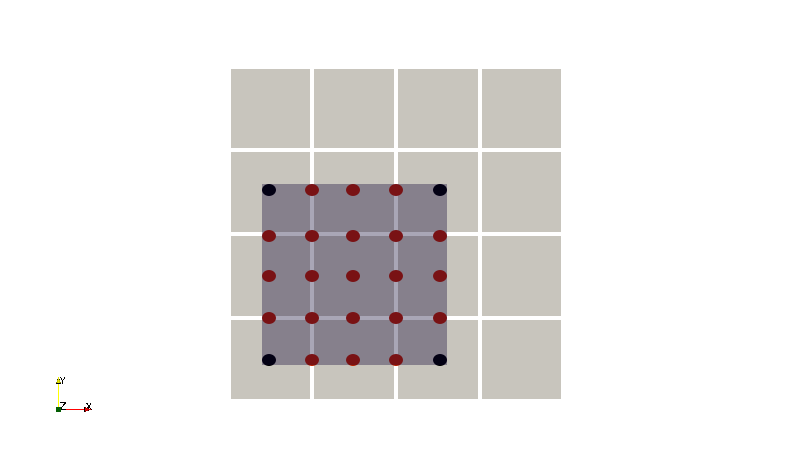
\includegraphics[width=1.2\linewidth]{Theory/fine_over_1.png}
  \caption{Subdomain for $p=2$ on a conforming mesh}
  \label{fine_over_1}
\end{subfigure}%
\begin{subfigure}{.5\textwidth}
  \centering
  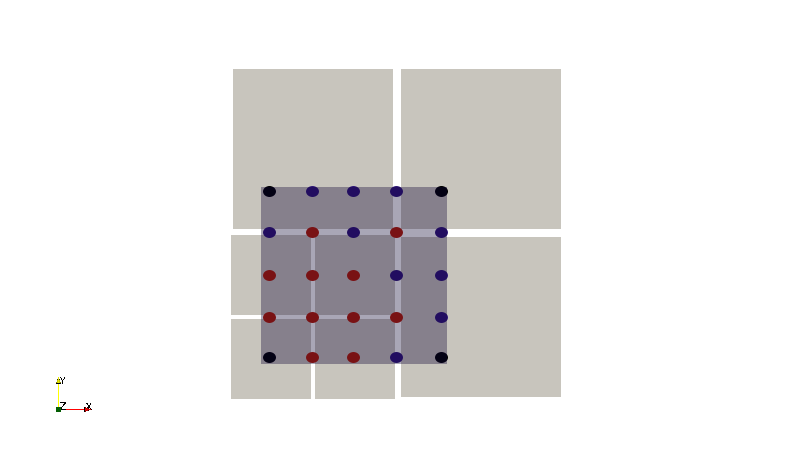
\includegraphics[width=1.2\linewidth]{Theory/fine_over_2.png}
  \caption{Subdomain for $p=2$ on a non conforming mesh}
  \label{fine_over_2}
\end{subfigure}
\caption{Example of two subdomains for $p=2$ used in the overlapping Schwarz preconditioner. On the left, we have a conforming mesh and all the local nodes are also global nodes (red). On the right, we have a non conforming mesh. Some nodes coincide with global GLL nodes (in red) but for others (in blue), we must use an interpolation to get their value. For both, the nodes at the corners of the subdomain (in black) will have a special treatment.}
\label{fine_over}
\end{figure}

We need to divide the mesh into overlapping subdomains. A natural choice is to use the quadrants and add a layer of GLL nodes to each side from neighboring quadrants. That yields $(p+3)^2$ local nodes on each subdomain. 

An example of the subdomains for $p=2$ is given in figure \ref{fine_over}. On the left, the mesh is conforming. That means that all the local nodes on subdomain $s$ coincide with global nodes. However, in a non conforming mesh, in addition to hanging nodes on some edges, we also need to interpolate the residual when, as presented in figure \ref{fine_over_2}, we are hanging with respect to our neighbor. There is also need for interpolation when at least one of our neighbor has hanging nodes. We can see here that adding hanging nodes brings a lot of new complexities. We will explain in more detail how they are treated in the implementation chapter. 

For now, let us assume that we have an operator $T_{ij;s}$ that gives the value of the local residual at local nodes $(i,j)$ on subdomain $s$. If we denote the global residual by $r$ and its restriction on subdomain $s$ by $r_{ij;s}$, then we have : 

\begin{align*}
r_{ij;s} &= T_{ij;s}r &\text{for $i,j=-1,0,...,p,p+1$} 
\end{align*}

Let us also note that, even in the conforming case, it is not always possible to compute the residual at the four corners of the subdomain (nodes in black on figure \ref{fine_over_1}). That is because in an unstructured mesh, a quadrant can have several other quadrants as neighbors through a corner or none at all. Therefore, we will impose that :

\begin{align*}
r_{ij;s} &= 0  &\text{at the four corners of the subdomain}
\end{align*} 

\subsection{Additive Schwarz method}

A more detailled explanation of the additive Schwarz method and the domain decomposition can be found in \cite{fine_book}. As said earlier, we now want to solve problem \ref{eq:poisson} to get the local fine scale correction, denoted by $z_{ij;s}$. In order to do this, we will impose homogeneous Dirichlet boundary conditions on nodes located at $i,j = -2$ or $i,j= p+2$.

As explained in \textcolor{red}{ref here}, since we are using the additive Schwarz method as a preconditioner, we do not need to be extremely accurate in the solution of problem \ref{eq:poisson}. We will also make an assumption that will allow us to compute the fine scale correction efficiently : we will assume that every quadrant is aligned with the axes. That means that a lot of geometric factors cancel and we can actually solve the problem analytically.

Let us first consider the equivalent 1D problem for an element of length $h$. The stiffness matrix is then given by : 

$$A^e_{ij} = \int_0^h  \frac{dl_i}{dx}\frac{dl_j}{dx} dx \approx \frac{2}{h} \sum_{m=0}^p w_mH_{im}H_{jm} = \frac{2}{h} d_{ij}$$

The influence of the overlaps (points at $-1$ and $p+1$) is computed using the standard finite element procedure : by adding their contribution to the stiffness matrix. We also assume that the neighboring elements have the same size so that the factor $h$ does not change. As a result, the linear system we obtain with the discretization is given by : 

\begin{align*}
A&= \begin{pmatrix}
d_{11} & d_{01} & 0 & \hdots & \hdots &\hdots & 0\\
d_{10} & 2d_{00} & d_{01} & \hdots & \hdots & d_{0p} & 0 \\
0 & d_{10} & d_{11} & \hdots & \hdots & d_{1p} & 0\\
\vdots & \vdots & \ddots & \ddots & \ddots & \vdots &\vdots \\
0 & d_{p-1,0} & \hdots & \hdots & d_{p-1,p-1} & d_{p-1,p} & 0\\
0 & d_{p0} & \hdots & \hdots & d_{p,p-1} & 2d_{pp} & d_{p-1,p}\\
0 & \hdots & \hdots & \hdots & 0 & d_{p,p-1} & d_{p-1,p-1}
\end{pmatrix}\\
M &= \begin{pmatrix}
w_1 & & & & & & \\
& 2w_0 & & & & & \\
& & w_1 & & & & \\
& & & \ddots & & &\\
& & & & w_{p-1} & &\\
& & & & & 2w_p & \\
& & & & & & w_{p-1}
\end{pmatrix}\\
\frac{4}{h^2}M^{-1}A z &= \frac{2}{h}M^{-1}r
\end{align*}

As mentioned in \textcolor{red}{ref here}, the matrix $L = M^{-1}A$ is diagonalizable and it has real and positive eigenvalues $\lambda_i$. So let us define : 

$$ L = V^{-1}\Lambda V$$

That leads to an analytic solution for $z$. Indeed : 

$$ z = \frac{h}{2} V^{-1}\Lambda^{-1}V M^{-1}r$$

Let us now try to generalize this procedure to the two dimensional case. As explained before, let us assume that the subdomain $s$ is aligned with the axes $x$ and $y$ and has dimension $h_x$ and $h_y$. Then the system of equations we have to solve to find the local fine scale correction on subdomain $s$, $z_{ij;s}$, is given by : 

\begin{align}
\sum_{m=-1}^{p+1} \frac{4}{h_x^2}L_{im}z_{mj;s} + \frac{4}{h_y^2} L_{jm}z_{im} &= \frac{4}{h_xh_y}\frac{1}{M_{ii}M_{jj}} r_{ij;s}  &\text{for $i,j=-1,...,p+1$} \label{eq:fine}
\end{align}

The reader can compare equation \ref{eq:fine} with the one derived in the section about the spectral element method to convince himself that it is indeed the set of equations obtained when the quadrant is aligned with the axes. 

Let us define the matrices $Z_s$ and $R'_s$  such that $(Z_s)_{ij} = z_{ij;s}$ and $(R'_s)_{ij} = \frac{4}{h_xh_y}\frac{1}{M_{ii}M_{jj}} r_{ij;s}$. Then, equation \ref{eq:fine} can be written as :

$$\frac{4}{h_x^2} LZ_s + \frac{4}{h_y^2} Z_sL^T = R'_s$$

Using the diagonalization of $L$, we have :

\begin{align}
\frac{4}{h_x^2} V^{-1}\Lambda V Z_s + \frac{4}{h_y^2} Z_s V^T\Lambda V^{-T} &= R'_s \nonumber \\
\frac{4}{h_x^2} \Lambda VZ_sV^T + \frac{4}{h_y^2} VZ_sV^T \lambda &= VR'_sV^T \label{eq:fine_inter}
\end{align}

Let us define $W = VZ_sV^T$ and $D=VR'_sV^T$. Then, it is obvious that the solution to equation \ref{eq:fine_inter} is given by : 

\begin{align*}
W_{ij} &= \frac{1}{\frac{4}{h_x^2}\lambda_i + \frac{4}{h_y^2}\lambda_j}D_{ij} &\text{for $i,j=-1,...,p+1$}\\
Z_s &= V^{-1}WV^{-T}
\end{align*}

We thus have reduced the problem to a few matrix products (where the matrices have $(p+3)$ rows and columns). If we had taken the geometric factors into account, we would have had a system with $(p+3)^2$ unknowns to solve for each subdomain $s$. That is $\mathcal{O}((p+3)^6)$ operations using a direct method. Here, we only need to perform matrix products and therefore we need $\mathcal{O}((p+3)^3)$ operations. The gain would be even greater in three dimensions. Let us note that the diagonalization of $L$ can be done once at the beginning since it does not depend on the subdomain.

The last thing we have to do is to gather the local fine preconditioner to the global GLL nodes to form the global fine preconditioner. As before, the gather operator is the transpose of the restriction operator. That yields : 

$$ P^f r = \sum_s \sum_{i=-1}^{p+1}\sum_{j=-1}^{p+1} T^T_{ij;s} z_{ij;s}$$

\subsection{Managing the actual boundary}

Up until now, we have assumed that the subdomain was included in $\Omega$. But some quadrants have at least an edge on $\Gamma$. In order to be able to use our analytic solution described above, we however need to give a value to the local fine residual. 

The method used here is to interpolate the value of the residual from inside the domain. For example, if the south edge is on the boundary $\Gamma$, then the local fine residual is given by : 

\begin{align*}
r_{i,-1;s} &= 2r_{i,0} - r_{i,1} &\text{for $i=0,...,p$}
\end{align*}

Of course, we do not gather the value of the fine scale correction that is outside of $\Omega$.











\chapter{Implementation}

The most important part of the work done in realizing this thesis was the implementation, from scratch, of the different methods presented in the theory chapter. It resulted in a code written in plain C and consisting of more than 8000 lines. 

Although it is impossible to present every part of the code here due to its shear volume, some parts are worth explaining. In this chapter, we will look into different the aspects of the implementation that are not immediately obvious.   

The first section of this chapter presents the $p4est$ library. It is an essential part of the implementation and it interacts with our application at all times. This is why we spend some time showing the components and the philosophy behind $p4est$. It is also important to understand the library to understand how we handle the mesh and its hanging nodes throughout the application.

The implementation of the spectral element method is quite straightforward. The only thing we present here is how to compute the $R_{ij}^e$ operator. 

The second section looks at the geometric multigrid method. The essential ingredient is a structure that handles all levels and the information needed on each. The building of such structure is presented here. 

The last section focuses on the implementation of the fine preconditioner. We show the different possible configurations as far as neighbors are concerned and we present how to compute the local residual in every case.  

\section{The p4est library}

Managing the mesh, especially when we have the presence of hanging nodes, is an important part of the work in any SEM implementation. This section thus present the library used, namely $p4est$ (the three dimensional equivalent is called $p8est$). 

The founding principles of $p4est$ are given in \cite{p4est}. In that article, they generate up to $5.13\: 10^{11}$ octants (the three dimensional equivalent of the quadrant) on as many as $2.2 \: 10^{5}$ CPU cores. Some additional information about the high-order node numbering can also be found in \cite{p4est2}. We present here only the features relevant to our work. 

We first present the approach to AMR used by $p4est$ and how it manages the dynamic refinement process, namely the refine and coarsen operators. We also explain the different structures used to build the mesh and the inherent terminology. 

In the second part, we will describe how, in our program, we handle hanging nodes leveraging $p4est$ and its structures. The way to compute the operator $R_{ij}^e$ (defined in the theory chapter) is also laid out. 

\subsection{AMR for p4est}

Different approaches exists for handling non conforming meshes. One strategy consists of splitting the computational domain into several unstructured macro-elements and then to refine them uniformly. The adaptivity is therefore only present at the coarse level. On the other hand, completely unstructured AMR yields more flexibility in the geometry but at a greater cost since there is no structure to rely on. Between the two are three-based methods, where each node is a quadrant that can have four children (which in turn can have children,...) or none at all. That recursive definition provides both simplicity and efficiency.

One downside is that the domain represented by a quadtree (a tree where a node is a leaf or has four children, as presented above) is always cube shaped. We can circumvent this problem by using a forest of quadtrees to represent a large range of geometrical shapes. 

The approach favored by $p4est$ is the latter : it handles the dynamic management of a collection of adaptive quadtrees, later called a forest of quadtrees. 

We can split the process used by $p4est$ in a two-level decomposition of the domain : first the definition of the forest, which we later call the macro-mesh, and then the adaptive recursive definition of each individual quadtree, later called the micro-mesh.

For the macro-mesh, the domain $\Omega \subset \mathbb{R}^2$ is split into $K$ conforming elements. Using $K$ conforming elements allows us to map more general domains than with a single quadtree since each corner of the macro-elements can be shared by more than 4 elements. There exists a mapping to each element from a reference element by a smooth function $\phi_k : [0;2^b]^2 \rightarrow \mathbb{R}^2$. Formally, we have that the domain $\Omega$ is split as : 

\begin{align*}
\Omega &= \bigcup_k \phi_k([0;2^b]^2) &0\leq k < K
\end{align*} 

We have an important thing to note here. It is an important feature of $p4est$ to perform all computations related to the connectivity and neighborhood relations discretely (i.e. it uses an integer-based approach). This is why the reference element is $[0;2^b]^2$. The main objective is to avoid floating-point arithmetic and the roundoff errors that might lead to errors in the topology. In their algorithms, the mappings $\phi_k$ are never used, except for the visualization and to encode the geometry that might be used for an external numerical application (such as ours). The consequence of having an integer-based system is that we cannot refine a quadtree indefinitely. Indeed, a quadrant cannot have a smaller length than 1 on the reference element. Thus, with $[0;2^b]^2$, it is possible to have at most $2^{2b}$ quadrants per element of the macro-mesh. Equivalently, each quadtree cannot have a depth superior to $b$, and a quadrant a refinement level superior to $b$. In the $p4est$ library, $b=29$, which yields a maximum of $2.9 \: 10^{17}$ quadrants per quadtree (the number would even be higher in three dimensions). We can see that it is amply sufficient for our applications. 

Let us also note that the macro-mesh cannot be changed dynamically and is shared among all processes. In practice, the number of quadtrees $K$ is thus limited by local memory. The experiments in \cite{p4est} go up to several million quadtrees.

Let us now turn to the micro-mesh. Based on a user-defined criterion, the refinement of the quadtree is often defined recursively. This creates a quadtree with the quadrants as leaves. Each quadrant of a given quadtree is then uniquely defined by the integer coordinates of its lower left corner $x,y \in \{0,1,2,...,2^b-1\}$ on the referent element and its level of refinement, i.e. the level of the leaf corresponding to that quadrant in the quadtree. In the reference element, a quadrant of level $l$ is a square of length $2^{b-l}$.


The details of the refine algorithm used in $p4est$ are not given here but can be found in \cite{p4est}. Here, non conforming edges are allowed. As mentioned in the theory chapter, our application only allows $1$-irregular meshes, i.e. two neighboring quadrants differ by at most one level of refinement. However, the refine function in $p4est$ does not constraint the size relations for neighboring quadrants (leading possibly to $k$-irregular meshes with $k>1$). Fortunately, the library also contains a balance function that we can use to guarantee a $1$-irregular mesh. Of course, the balance function acts both on quadrants in the same quadtree and on quadrants in different quadtrees that connect through an edge of the macro-mesh. 

The micro-mesh, i.e. the collection of quadrants, can be dynamically changed (with the refine and coarsen functions) and is shared between all processes. 

\begin{figure}
\centering
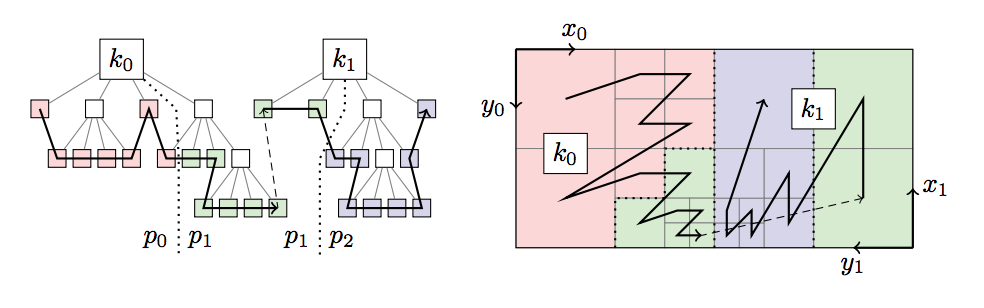
\includegraphics[scale=1.0]{Implementation/filling_curve.png}
\caption{One-to-one correspondence between a forest of quadtrees (left) and a computational domain (right). There are two quadtrees $k_0$ and $k_1$ (corresponding to two elements in the macro-mesh). Going through the leaves of the forest from left to right creates a space filling curve (in black) and thus a total ordering of the quadrants. Source : \cite{p4est}. }
\label{filling_curve}
\end{figure}

Tree-based AMR methods naturally lead to space filling curves. Indeed, if the global index of a quadrant is given by its order of appearance when looking at the forest of quatrees from left to right, then going quadrant by quadrant creates a curves that tends to fill the domain. An example of this is given in figure \ref{filling_curve}. On the left, we can see the forest which contains two quadtree ($k_0$ and $k_1$), distributed between three processes. We can also see that the refinement process has lead to quadrants with level 1, 2 and 3. On the right, the corresponding mesh is shown. Because we have different levels of refinement, the mesh is non conforming but it is still acceptable for our application since it is $1$-irregular. Inspecting the leaves in the forest of quadtrees from left to right creates a space filling curve that can be used to define a global index for the quadrants. We can see that, within one quadtree, the space filling curve follows the orientation of its coordinate axes.

There are still three things we want to point out in this part : how to tell if a quadrant is touching the boundary of the computational domain, how to obtain the physical coordinates of the corners of any quadrant and give some explanation about the global numbering of nodes used in the spectral elements method. 

\subsubsection{Quadrants on the boundary}

When we solve the system arising from SEM, it is fundamental to be able to tell whether a quadrant has one of its face on the boundary of the computational domain. 

Let us first note that if a quadrant has a face on the boundary, then the corresponding face of the macro-mesh element is on the boundary. 

In order to be able to tell about the neighboring quadtrees, there exists a function $k'=NO(k,f)$ that tells for a quadtree $k$ that its neighbor through face $f$ is $k'$, as well as a function $f' = NF(k,f)$ that tells that $k'$ is connected to $k$ through face $f'$. 

The convention used by $p4est$ to say that quadtree $k$ has face $f$ on the boundary is : 

\begin{align*}
NO(k,f) &= k\\
NF(k,f) &= f
\end{align*}

This convention only prevents the (pathological!) configuration where a quadtree connects to itself periodically through a face that is rotated against itself and that never happens in our application. That enables us to tell which quadrants have a face on the boundary. 

\subsubsection{Physical coordinates of the corners}

We are now looking at how to compute the physical coordinates of a quadrant. Let us first define the one dimensional linear mapping : 

\begin{align*}
\phi_0(x) &= 1-x\\
\phi_1(x) &= x
\end{align*}

Let us then assume that the quadrant is located in the macro-mesh element $k$. Let us also denote the physical coordinates of the corners of element $k$ by $x^k_i,y^k_i$ for $i=0,1,2,3$. Let us finally assume that the integer-based coordinate of the lower left corner of the quadrant are $x,y$ and it has a level of refinement $l$. In the reference element, the quadrant has therefore a length of :

$$ h = 2^{b-l} $$ 

Let us then use our linear mapping above to compute the coordinates of the corners of the quadrant $X_i,Y_i$ for $i=0,1,2,3$ as : 

\begin{align*}
X_{i+2j} &= \sum_{i=0}^1\sum_{j=0}^1 x^k_{i+2j} \phi_i(\frac{x+ih}{2^b})\phi_j(\frac{x+jh}{2^b}) &\text{for $i,j=0,1$}\\ 
Y_{i+2j} &= \sum_{i=0}^1\sum_{j=0}^1 y^k_{i+2j} \phi_i(\frac{x+ih}{2^b})\phi_j(\frac{x+jh}{2^b}) &\text{for $i,j=0,1$}\\ 
\end{align*}


Once we have the physical coordinates of any quadrants of our mesh, we can compute easily quantities such as the physical coordinates of the different local GLL nodes, the value of the jacobian,...

\subsubsection{Global unique node numbering}

Let us finally give some explanation about the globally unique numbering of the unknowns used in the spectral elements method. It is created in $p4est$ by a structure named $lnodes$. The principle is to number in order the global GLL nodes encountered while going through the quadrants by the global index. If there are no hanging nodes, it is simple : when we get to a quadrant, we number the nodes that have still not been numbered in lexicographic order then go to the next quadrant. When we have hanging nodes, it is more difficult since they are not independent and therefore cannot get a global numbering. The principle is then to number the global nodes that have an influence of the hanging nodes in the quadrant. 

\begin{figure}
\centering
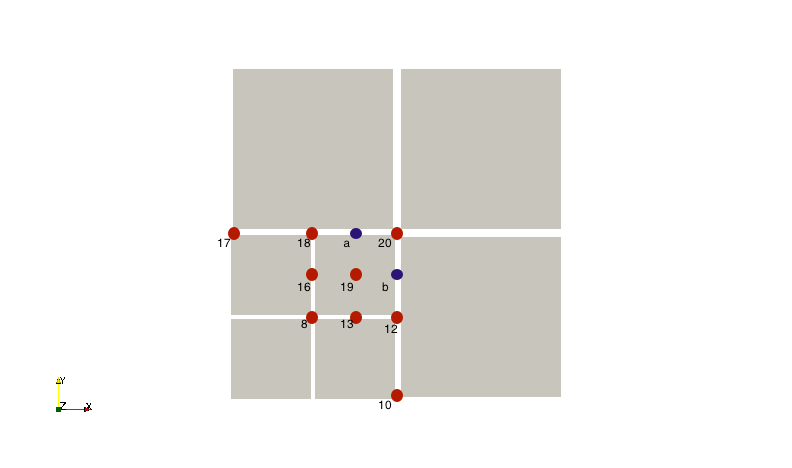
\includegraphics[scale=0.5]{Implementation/nodes_ex.png}
\caption{Global numbering of the nodes (in red) that have an influence in the small quadrant close to the center as well as the hanging nodes (in blue) for an interpolation of degree $p=2$. }
\label{nodes_ex}
\end{figure}

All this information is contained in a large array called $element\_nodes$ in $lnodes$. Let us give an example for the sake of clarity. Figure \ref{nodes_ex} shows a mesh for a degree of interpolation $p=2$ where we see in red the global nodes having an influence in the small quadrant close to the center. We can see that this quadrant has two hanging edges. The $element\_nodes$ array for this example is given by : 

$$element\_nodes = \begin{bmatrix}
8 &13& 10& 16 &19& 12 &17& 18& 20
\end{bmatrix}$$

We can see that it numbers the global GLL nodes first in the $x$ direction, then in the $y$ direction and uses the global numbering to refer to hanging nodes. It is possible to do this since hanging nodes are always located on edges. 

\subsection{Handling the hanging nodes}

Let us now look at how to practically handle hanging nodes. As presented before, the array $element\_nodes$ always uses global numbering to tell the nodes that have an influence in a quadrant. Therefore, we have to know which, if any, edges are hanging. This information, for each quadrant, is encoded in $face\_code$ in $lnodes$.

\subsubsection{Decoding the face code}

The function that we built to decode $face\_code$ returns $false$ if no edge is hanging while it returns $true$ and fill an array of length 4 called $hanging\_corner$ if there are at least one hanging edge where : 

\begin{align*}
hanging\_corner_i &= -1 &\text{if corner $i$ is not hanging}\\
&= a &\text{if $a$ is the non hanging corner corresponding to $i$}
\end{align*}

The $face\_code$ is a bitcode where the last two bits contain the position of the quadrant relative to its parent and the next two bits contain the status of the potentially hanging edges. Indeed, it is obvious that for any quadrant, at most two edges can be hanging. 

For example, in figure \ref{nodes_ex}, the $face\_code$ of the quadrant is $1111$ since it is the fourth child of its parent and the two potentially hanging nodes are indeed hanging. The $hanging\_corner$ array resulting from decoding that face code is : 

$$hanging\_corner = \begin{bmatrix}
-1 &3& 3& -1
\end{bmatrix}$$

Once we have the hanging corners, we can know which edges are hanging and if those edges constitute the first or the second part of the corresponding non hanging edge. For example in figure \ref{nodes_ex}, the east edge is hanging and constitute the second part of the corresponding non hanging edge defined by global nodes 10 and 20. 

\subsubsection{Computing $R_{ij}^e$}

All the information about the mesh computed above has two purposes : for us to be able to interpolate the different functions in each quadrant (scatter operation) and then to gather the result of the integration. As mentioned in the theory chapter, we never build the operator $R_{ij}^e$ explicitly. Let us first present the scatter operation. There are three positions possible for a local GLL node : 

\begin{enumerate}
\item The node is one of the four corners
\item The node is on an edge
\item The node is in the "interior", i.e. neither on an edge nor on a corner
\end{enumerate}

Let us stress the fact that only the first two types of nodes can be hanging. Therefore, the first step every time we need to perform an interpolation is to load the "interior", since we are sure those nodes are not hanging. In figure \ref{nodes_ex}, this corresponds to only one node (19).

The second step is to look at the edges. If an edge is not hanging, then we can load all nodes on this edge but the corners (since even on a non hanging edge, those can be hanging). In figure \ref{nodes_ex}, this corresponds to node 13 for the south edge and node 16 for the west edge. For the hanging edges, we need to perform an interpolation of the values at the global nodes to obtain the values at the hanging nodes. We can do a one dimensional interpolation since hanging nodes and the global nodes that influence them are located along an edge which is a straight line. In figure \ref{nodes_ex}, hanging nodes $b$ is interpolated using global nodes 10, 12 and 20.  Whether the hanging edge is the first or the second part of the non hanging edge is important since the interpolation will be different. Let us assume that the values at the global nodes are given by $u^{glob}_i$ for $i=0,...,p$. Then the value at hanging node $j$, $u^{loc}_j$, is given by : 

\begin{align*}
u^{loc}_j &= \sum_{k=0}^p l_k\left(\frac{\xi_j}{2}-\frac{1}{2}\right) u_k^{glob} &\text{if the hanging edge constitutes the first part}\\
u^{loc}_j &= \sum_{k=0}^p l_k\left(\frac{\xi_j}{2}+\frac{1}{2}\right) u_k^{glob} &\text{if the hanging edge constitutes the second part}
\end{align*}

Where $l_k$ denotes the Lagrangian polynomial associated with the $k$-th 1D GLL node. Since it is always the same interpolation (i.e. the coefficients of the linear combination do not depend on the quadrant) for all hanging edges, we built two matrices that perform the interpolation (one when the edge is the first part, $D^1$, and the other when the edge is the second part, $D^2$) and we use them every time we have a hanging edge. 

\begin{align*}
D^1_{ij} &= l_j\left(\frac{\xi_i}{2}-\frac{1}{2}\right)\\
D^2_{ij} &= l_j\left(\frac{\xi_i}{2}+\frac{1}{2}\right)
\end{align*}

For the example given in figure \ref{nodes_ex}, we have for the east edge :

$$ \begin{pmatrix}
u_{12} \\ u_b \\ u_{20}
\end{pmatrix} = \begin{pmatrix}
0 & 1 & 0\\
-0.125 & 0.75 & 0.375\\
0 & 0 & 1
\end{pmatrix}\begin{pmatrix}
u_{10} \\ u_{12} \\ u_{20}
\end{pmatrix}$$

Here we can also do the corners and mark them as visited.

The third step is to look at all four corners and check whether we have visited them or not. Those we have not yet visited are not hanging and we can therefore load them. In figure \ref{nodes_ex}, this corresponds to node 8. 

The gather operation works in much the same way. We first deal with the interior where we are sure no nodes are hanging. Then, we look at the edges. If the edge is hanging, we use the transpose of the matrices $D^1$ and $D^2$ to go from local nodes to global ones. We end with the corners that have not yet been visited. 



\section{Multigrid structure}

Let us now move on the structure used to handle the multigrid method. Is it the most important structure to build. If we define our structure in the right way, smoothing, restricting and prolonging are fairly straightforward.

Let us first note that throughout the program, we have two different global node numbering. One for the high degree interpolation, $lnodesP$, and one for the interpolation with $p=1$ used in the multigrid, $lnodes1$. As expalined in the theory chapter, we therefore need functions to transfer the high degree residual from $lnodesP$ to $lnodes1$ and then to transfer the coarse grid correction from $lnodes1$ to $lnodesP$. The details of that transfer are not given here but the implementation from the theory is rather simple. 

We will focus here on the structure we build to handle the multigrid using the global numbering used by $lnodes1$. For each level, we need to know : 

\begin{enumerate}
\item The number of nodes on that level
\item The number of quadrants on that level
\item Which nodes form the $k$-th quadrant
\item If a given quadrant has children on the upper level and if so, which quadrants they are
\item What quadrants are hanging on that level
\item The hanging information of the hanging quadrants
\end{enumerate} 

Several other arrays are also contained in the structure to store the value of the solution at that level, the right-hand side, some geometric factors, ...

Building the structure is a two-step process : we first fill the highest level (corresponding to the finest grid) and then we recursively fill the levels by the information contained in the upper level (we use level $lev+1$ to fill level $lev$).

\subsection{Filling the highest level}

At the highest level, called $maxlev$, it is obvious that the number of nodes, $N^{maxlev}$, is the number of nodes in $lnodes1$, the number of quadrants, $Q^{maxlev}$, is the number of quadrants in the forest and the nodes for the $k$-th quadrant, $nodes^{maxlev}_{i;k}$, are given by $element\_nodes$ in $lnodes1$. There is no upper level so we do not need to care about the children (the array $up^{maxlev}$ is set to -1).

We then have an array containing boolean flags to see if quadrant $k$ has hanging nodes. This is easy to see from the $face\_code$ (see above).

\begin{align*}
hang_k^{maxlev} &= 1 &\text{if quadrant $k$ contains hanging nodes}\\
&= 0 &\text{if quadrant $k$ does not contain hanging nodes} 
\end{align*} 

For quadrants where there is at least one hanging node, we decode the $face\_code$ using the function defined in the previous section and we store the information. 

\begin{align*}
hang\_info^{maxlev}_{i;k} &= -1 &\text{if corner $i$ in quadrant $k$ is not hanging}\\
 &= a &\text{if $a$ is the non hanging corner corresponding to $i$}
\end{align*}

\subsection{Recursively filling the lower levels}

\begin{figure}
\centering
\begin{subfigure}{.5\textwidth}
  \centering
  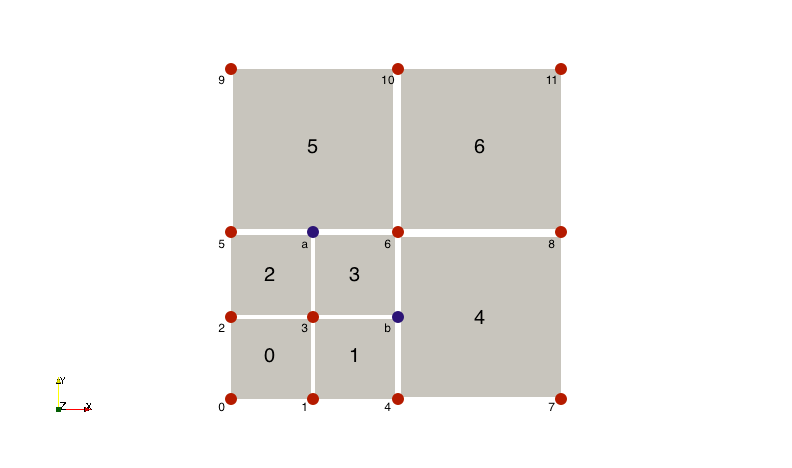
\includegraphics[width=1.2\linewidth]{Implementation/multi_ex_2.png}
  \caption{Mesh at level 2}
  \label{multi_ex_2}
\end{subfigure}%
\begin{subfigure}{.5\textwidth}
  \centering
  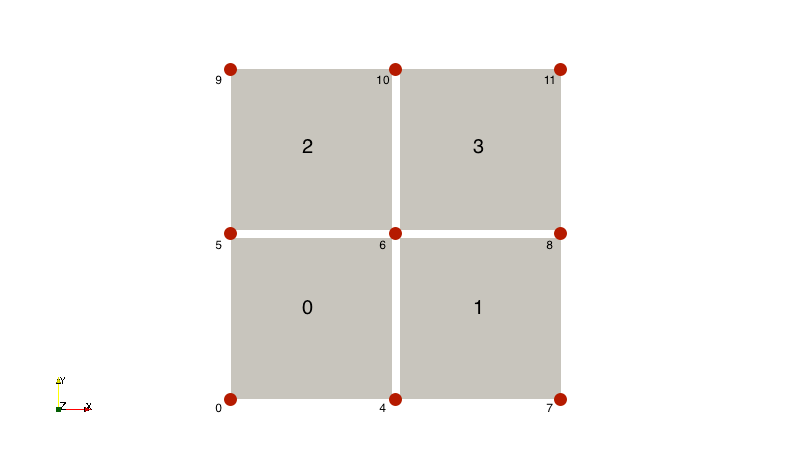
\includegraphics[width=1.2\linewidth]{Implementation/multi_ex_1.png}
  \caption{Mesh at level 1}
  \label{multi_ex_1}
\end{subfigure}
\caption{Example of two meshes at level 1 and 2. We can see that when we go from level 2 to level 1, all quadrants that had a refinement level of 2 are replaced by their parent. Moreover, the parent of the quadrants with level of refinement 2 that were hanging at level 2 is not hanging at level 1. The global nodes are in red (with their global number) and the hanging nodes in blue. The global number of the quadrants is also given.}
\label{multi_ex}
\end{figure}

Let us remember that the mesh at level $lev$ is the mesh at level $lev+1$ where all quadrants with level of refinement $lev+1$ have been replaced by their parent. We can see an example in figure \ref{multi_ex}. At level 1, all quadrants with level 2 have been replaced by their parent.

An important thing to note here is that if a quadrant with level of refinement $lev+1$ is hanging at level $lev+1$, then the corresponding parent at level $lev$ is not hanging. This is a direct consequence of the fact that two neighboring quadrants differ by at most one level in their refinement levels. In the example in figure \ref{multi_ex}, we can indeed see that the parent of the quadrants that were hanging at level 2 is not hanging at level 1.

The first thing to do is to compute the number of quadrants at level $lev$. If, at level $lev+1$, there are $q^{lev+1}$ quadrants with a level of refinement of $lev+1$, then it is given by : 

$$Q^{lev} = Q^{lev+1} - \frac{3}{4} q^{lev+1}$$

Then, we go quadrant by quadrant following their global ordering (given by the space-filling curve). If the current quadrant has a refinement level inferior or equal to $lev$, then we copy the information from level $lev+1$ to level $lev$. However, if we reach a quadrant with a refinement level of $lev+1$, then we have to coarsen. An important thing to note is that, if we visit the quadrants in their global order given by the space filling curve, then the four quadrants we have to replace by their parent when we coarsen are always positioned consecutively. Therefore, we can fill the $up$ array easily. For the example in figure \ref{multi_ex}, we have :

$$up^1_0 = \begin{bmatrix}
0 & 1 & 2 & 3
\end{bmatrix}$$

The $up$ array for the other quadrants are filled with -1 since they do not have children. We can also use the fact that the children are placed consecutively and the fact that when we coarsen we are sure that no node is hanging to easily fill the $nodes$ array. In our example this yields : 

\begin{align*}
nodes^1_0 &= \begin{bmatrix}
nodes^2_{0;0} & nodes^2_{1;1} & nodes^2_{2;2} & nodes^2_{3;3}
\end{bmatrix}\\
&= \begin{bmatrix}
0 & 4 & 5 & 6
\end{bmatrix}
\end{align*}

The last thing to handle for that set of quadrants is the hanging information. Since we coarsen, the parent is not hanging. In our example, that just means setting $hang^1_0 = 0$. 

After having gone through all the quadrants, we still need to compute the number of global nodes at level $lev$. The idea is to fill an array with all the nodes we see when we go through the quadrants (which is therefore of length $4Q^{lev}$), then to sort this array and count the number of different global nodes we have. That also allows us to set up a mapping between the numbering of the nodes at level $lev$ and the global numbering given in $lnodes1$. That mapping is very useful when we have to perform an operation on the nodes at a given level (for example, during the smoothing). 
 
Let us finally say that the minimum level ($lev = 0$) is the macro-mesh. It is a conforming mesh and on it, we solve the linear system of equation exactly using the Lapack library (see \cite{lapack} for information).  
 














\chapter{Results and discussion}
In this chapter, we will present the different results and discuss them.

\textcolor{red}{Expliquer ce qu'on va faire et tester}

\textcolor{red}{Mettre ici les trois "super mesh"}
\section{Multigrid}
In this section, we will test the coarse part of the preconditioner : the multigrid solver. This will be done in two steps. First, we will verify a well known property of the multigrid solvers : the h-independent convergence. We will also compare the number and iterations needed while varying key parameters of the model. Those tests will be performed on various meshes. The second part will focus on the influence of hanging nodes on the numerical solution. 

Let us before all present a type of numerical solution that can be obtained using the multigrid solver. Figure \ref{multi_simple_sol} shows an example of the numerical solution computed. We can see that even with $p=1$, we have a good approximation. This is because the forcing term is not at all oscillatory.

\begin{figure}
\centering
\includegraphics[scale=0.35]{Results/multi_simple_sol.eps}
\caption{Numerical solution using the multigrid solver of $\nabla^2 u = f$ for $f = -2\tanh(3x)\tanh(3y)(18-9\tanh^2(3x)-9\tanh^2(3y))$}
\label{multi_simple_sol}
\end{figure}

\subsection{H-independent convergence}
Let us first verify that our geometric multigrid solver has the required property and that the same number of iterations is needed to obtain a given accuracy, however small the elements. We will use the model problem throughout this section with the same right hand side. For all the tests below, the domain  will be : $\Omega = [-1;1]^2$. We will solve : 

\begin{align}
\nabla^2 u &= -\frac{\pi^2}{2}\cos(\frac{\pi}{2}x)\cos(\frac{\pi}{2}y) &\text{on $\Omega$} \\
u &= 0  &\text{on $\Gamma$}
\end{align}

It is easy to see that for the given domain, we have an analytic solution : 
$$u(x,y) = \cos(\frac{\pi}{2}x)\cos(\frac{\pi}{2}y))$$ 


Let us now explain how we define the error. We will look at the absolute difference between the value of the approximation and the value of the analytic solution at the global nodes and take the maximum. Formally, we have that the error after iteration $k$, $e_k$ is :

$$e_k = \max_i |u(x_i,y_i) - u_i^k|$$

Where $u_i^k$ is the value of our approximation at the global node $i$ after iteration $k$. Since $u_i^0 = 0$ for all $i$, it is clear that $e_0 = 1$.

Figure \ref{multi_mesh} shows the two "supra meshes" that we will refine during the tests. Some refinements will be uniform and some will be so that we have the presence of hanging nodes. We can note that even for the crooked mesh, the elements are not really distorted. It does not matter since we are only testing the h-independent convergence. Having a mesh with elements that are more distorted will only influence the accuracy of the approximation and not how the algorithm solve the linear system we want to solve. 

\begin{figure}
\centering
\begin{subfigure}{.5\textwidth}
  \centering
  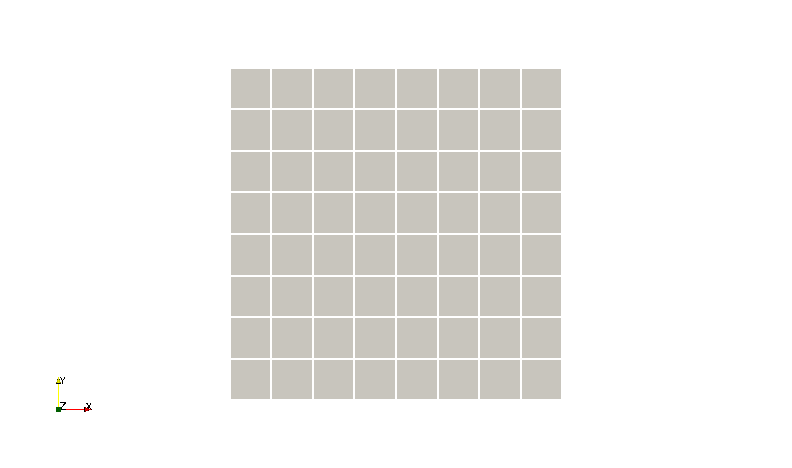
\includegraphics[width=1.2\linewidth]{Results/multi_mesh_1.png}
  \caption{Regular mesh}
  \label{multi_mesh_1}
\end{subfigure}%
\begin{subfigure}{.5\textwidth}
  \centering
  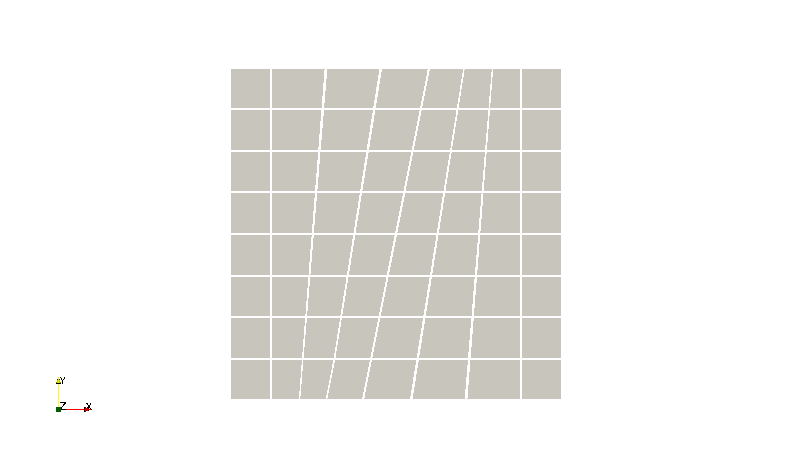
\includegraphics[width=1.2\linewidth]{Results/multi_mesh_2.png}
  \caption{Crooked mesh}
  \label{multi_mesh_2}
\end{subfigure}
\caption{The two "supra meshes" that will be refined during the tests for the multigrid solver. We have one regular mesh (left) where the elements are squares and one crooked mesh (right) where the elements are slightly distorted.}
\label{multi_mesh}
\end{figure}



Let us start with a simple V-cycle on the regular mesh (figure \ref{multi_mesh_1}) that we will refine uniformly. We will compare the errors when we increase the number of degrees of freedom and for different $\nu_1$ and $\nu_2$. The sum of the two smoothing parameters is chosen to be constant so that we have the same number of Jacobi iterations for all pairs $\nu_1$ and $\nu_2$. Here, we chose the sum to be equal to four.


\begin{table}
\centering
\begin{tabular}{c|ccccc}
\hline
 N & $2.6\:10^5$ & $1.1\:10^6$ & $4.2\: 10^6$& $1.7\:10^7$ & $6.7\:10^7$ \\
 \hline
  & $\nu_1=2$ & $\nu_2=2$ & & &\\
  \hline
  $e_1$ & 3.56e-02 & 3.56e-02 & 3.56e-02 & 3.56e-02 & 3.56e-02\\
  $e_2$ & 1.34e-03 &	1.34e-03 &	1.34e-03	& 1.34e-03	& 1.34e-03\\
  $e_3$ & 5.42e-05 &	5.66e-05 &	5.72e-05 &	5.73e-05 &	5.73e-05\\
  $e_4$ & 3.11e-06 &	2.90e-06 &	3.45e-06 &	3.59e-06 &	3.62e-06\\
  $e_5$ & 3.30e-06 &	9.48e-07 &	3.62e-07	& 3.50e-07 &	3.85e-07\\
  $e_6$ & 3.17e-06 &	8.14e-07 &	2.26e-07 &	8.26e-08 &	5.23e-08\\
  \hline
  & $\nu_1=3$ & $\nu_2=1$ & & &\\
  \hline
  $e_1$ & 3.70e-02 &	3.71e-02 &	3.71e-02 &	3.71e-02 &	3.71e-02\\
  $e_2$ & 1.62e-03 &	1.63e-03 &	1.63e-03 &	1.63e-03 &	1.63e-03\\
  $e_3$ & 1.04e-04 &	1.06e-04 &	1.07e-04 &	1.07e-04	& 1.07e-04\\
  $e_4$ & 1.10e-05 &	1.22e-05 &	1.27e-05 &	1.29e-05 & 	1.29e-05\\
  $e_5$ & 4.47e-06 &	2.20e-06 &	1.96e-06 &	2.10e-06 & 	2.13e-06\\
  $e_6$ & 3.34e-06 &	1.00e-06 &	4.38e-07 &	3.53e-07 &	3.88e-07\\
  \hline
  & $\nu_1=1$ & $\nu_2=3$ & & &\\
  \hline
  $e_1$ & 3.57e-02 &	3.57e-02 &	3.57e-02 &	3.57e-02 &	3.57e-02\\
  $e_2$ & 1.29e-03 &	1.29e-03 &	1.29e-03 &	1.29e-03 &	1.29e-03\\
  $e_3$ & 4.66e-05 &	4.89e-05 &	4.95e-05 &	4.96e-05 &	4.97e-05\\
  $e_4$ & 1.53e-06 &	1.53e-06 &	2.10e-06 &	2.24e-06 &	2.28e-06\\
  $e_5$ & 3.08e-06 &	7.31e-07 &	1.43e-07 &	1.17e-07 &	1.51e-07\\
  $e_6$ & 3.14e-06 &	7.83e-07 &	1.95e-07 &	4.80e-08 &	1.13e-08\\
  \hline
   & $\nu_1=4$ & $\nu_2=0$ & & &\\
  \hline
  $e_1$ & 4.55e-02 &	4.55e-02 &	4.55e-02 &	4.55e-02 &	4.55e-02\\
  $e_2$ & 3.26e-03 &	3.26e-03 &	3.26e-03 &	3.26e-03 &	3.26e-03\\
  $e_3$ & 4.64e-04 &	4.71e-04 &	4.71e-04 &	4.71e-04 &	4.71e-04\\
  $e_4$ & 9.24e-05 &	9.60e-05 &	9.65e-05 &	9.67e-05 &	9.67e-05\\
  $e_5$ & 1.74e-05 &	2.04e-05 &	2.12e-05 &	2.14e-05 &	2.14e-05\\
  $e_6$ & 6.17e-06 &	3.86e-06	& 4.55e-06	& 4.74e-06 &	4.78e-06\\
  \hline
  & $\nu_1=0$ & $\nu_2=4$ & & &\\
  \hline
  $e_1$ & 3.58e-02 &	3.58e-02 &	3.58e-02 &	3.58e-02 &	3.58e-02\\
  $e_2$ & 1.29e-03 &	1.29e-03 &	1.29e-03 &	1.29e-03 &	1.29e-03\\
  $e_3$ & 4.53e-05 &	4.77e-05 &	4.82e-05 &	4.84e-05 &	4.84e-05\\
  $e_4$ & 1.17e-06 &	1.31e-06 &	1.89e-06 &	2.03e-06 &	2.07e-06\\
  $e_5$ & 3.03e-06 &	6.80e-07 &	9.14e-08 &	7.66e-08 &	1.12e-07\\
  $e_6$ & 3.13e-06 &	7.76e-07 &	1.87e-07 &	4.04e-08 &	3.62e-09\\
  \hline
\end{tabular}
\caption{Errors after $k$ iterations of a V-cycle ($e_k$) for the regular mesh uniformly refined to have $N$ degrees of freedom and for different values of the parameters $\nu_1$ and $\nu_2$}
\label{multi_err_nu}
\end{table}

The results are shown in table \ref{multi_err_nu}. We can see that we indeed have an h-independent convergence of the solver. For every pair of the smoothing parameters, at least for the first few iterations, the error $e_k$ is identical for all values of $N$. Except for the pair $\nu_1 = 4$ and $\nu_2 = 0$, each iteration roughly decrease the error by one decimal point.

We can also note that the values of the parameters influence the convergence. For this particular problem and this particular mesh, the values $\nu_1 = 0$ and  $\nu_2 = 4$ seem to be the best as the error is smaller after the same number of iterations than for the other pairs. The less post smoothing iterations ($\nu_2$) we do, the slower the convergence. This is true for $\nu_2 = 1$ where the error on the finest mesh after six iterations is a hundred times larger than on the same mesh after the same number of iterations for $\nu_2=4$, and it is clearer still for $\nu_2=0$ where the error is a thousand times larger after six iterations on the finest mesh.

We have to note that even tough the errors are identical for all meshes at first, we have a difference after a few iterations. This can be explained by the fact that our geometric multigrid algorithm actually solves a linear system whereas the error is measured as the difference between the analytic solution and the solution of the linear system. Thus, even if we solved the linear system exactly, we would still have an error and that error should decrease as the number of degrees of freedom increases. This is indeed what we observe here. For example, for the mesh with $N=2.6\:10^5$, we can see that after six iterations, we have almost converged and that the error stays around $3.14\:10^{-6}$. Even if we did several more iterations, the error would not decrease significantly. That is because we have the solution of the linear system and the error is only due to the discretization. If we refine the mesh and go to $N=6.7\:10^7$, then we can get smaller errors (of the order of $10^{-8}$).

Let us now explore the results for the crooked mesh (figure \ref{multi_mesh_2}). Here also, we should expect an h-independent convergence. We only show the results for $\nu_1=2$ and $\nu_2=2$ but the same commentary applies for the other pairs. The results can be seen on table \ref{multi_err_crook}

\begin{table}
\centering
\begin{tabular}{c|ccccc}
\hline
N & $2.6\:10^5$ & $1.1\:10^6$ & $4.2\: 10^6$& $1.7\:10^7$ & $6.7\:10^7$ \\
 \hline
  & $\nu_1=2$ & $\nu_2=2$ & & &\\
  \hline
  $e_1$ & 3.64e-02 &	3.64e-02 &	3.64e-02 &	3.64e-02 &	3.64e-02\\
  $e_2$ & 2.56e-03 &	2.49e-03 &	2.46e-03	& 2.44e-03 &	2.43e-03\\
  $e_3$ & 7.41e-04 &	6.33e-04 &	5.80e-04 &	5.54e-04 &	5.41e-04\\
  $e_4$ & 6.15e-04 &	3.15e-04 &	1.62e-04 &	1.35e-04 &	1.28e-04\\
  $e_5$ & 5.96e-04 &	3.01e-04 &	1.52e-04 &	7.67e-05	& 4.76e-05\\
  $e_6$ & 5.91e-04 &	2.98e-04 &	1.50e-04 &	7.50e-05 &	3.77e-05\\
  \hline
\end{tabular}
\caption{Errors after $k$ iterations of a V-cycle ($e_k$) for the crooked mesh uniformly refined to have $N$ degrees of freedom and for $\nu_1=2$ and $\nu_2=2$}
\label{multi_err_crook}
\end{table}

We can see that the for the first few iterations, the error $e_k$ is independent of the mesh. However, the note we made earlier is much clearer here. Because the mesh is not regular, the effect of discretization are more important and therefore we will not reach the same accuracy than we did before. That is why after six iterations, the less refined grid ($N = 2.6\:10^5$) still has an error of $5.91\:10^{-4}$. More iterations will not have a great impact on the solution since the error is mostly due to the discretization.

\subsection{Influence of hanging nodes}
We will now investigate the influence of hanging nodes on our solution. We will present the results only for the regular mesh but the tests have been performed on both and the same conclusions apply to the crooked mesh.

We will compare the values of the error between one mesh with no hanging nodes, one where we only have refined the lower left part of the domain once, and one where we have a rapid transition between two parts  of different refinement level (which will occur often in AMR).

Figure \ref{multi_mesh_hanging} presents the latter two meshes. For the mesh in figure \ref{multi_mesh_hanging_2}, we have refined thrice more in a certain region than in the adjacent one. Since we do not allow adjacent quadrants to be more than one level apart, we obtain a "layer" where the levels of the quadrants is rapidly changing. In order to compare solutions, we made sure that the largest quadrants in all three meshes had the same size. This means that the meshes with hanging nodes have a lot more degrees of freedom.  

\begin{figure}
\centering
\begin{subfigure}{.5\textwidth}
  \centering
  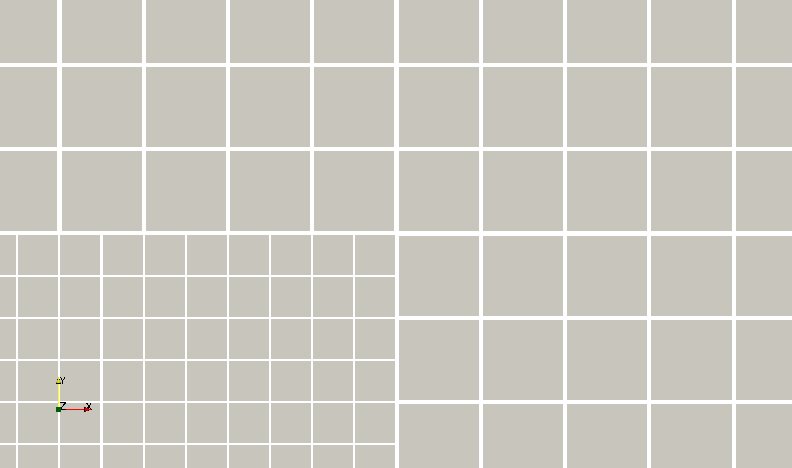
\includegraphics[width=0.8\linewidth]{Results/multi_mesh_hanging_1.png}
  \caption{Two levels}
  \label{multi_mesh_hanging_1}
\end{subfigure}%
\begin{subfigure}{.5\textwidth}
  \centering
  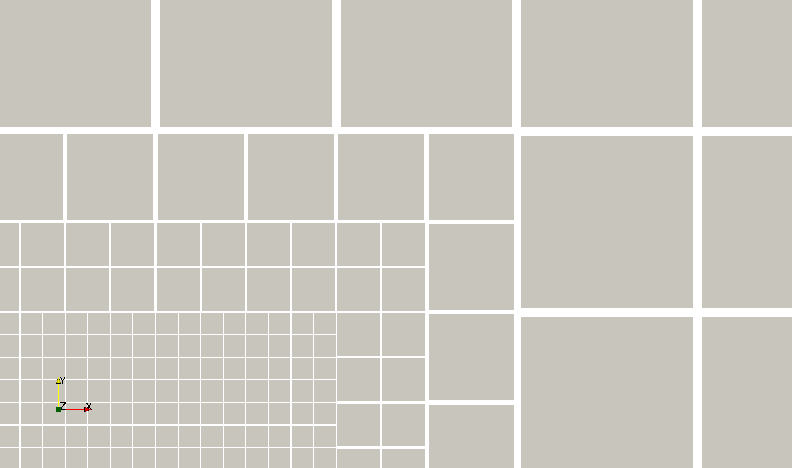
\includegraphics[width=0.8\linewidth]{Results/multi_mesh_hanging_2.png}
  \caption{Levels rapidly changing}
  \label{multi_mesh_hanging_2}
\end{subfigure}
\caption{Zoom on a certain part of the two meshes containing hanging nodes that will be used to test the multigrid solver. We have one mesh where we only have refined a part of the domain once more than the rest (left) and a mesh where we have refined a part thrice more than the rest which results in levels changing rapidly (right).}
\label{multi_mesh_hanging}
\end{figure}


\begin{table}
\centering
\begin{tabular}{c|ccc}
\hline
Meshes & No hanging nodes & Figure \ref{multi_mesh_hanging_1} & Figure \ref{multi_mesh_hanging_2}\\
\hline
N & $4.2\:10^6$ & $7.3\:10^6$ & $7.0\: 10^7$ \\
  \hline
  $e_1$ & 3.56e-02 &	3.56e-02 &	3.56e-02 \\
  $e_2$ & 1.34e-03 &	1.34e-03 &	1.34e-03	\\
  $e_3$ & 5.72e-05 &	5.72e-05 &	5.74e-05 \\
  $e_4$ & 3.45e-06 &	3.47e-06 &	3.64e-06 \\
  \hline
\end{tabular}
\caption{Errors after $k$ iterations of a V-cycle ($e_k$) for a mesh without hanging nodes and the two meshes presented in figure \ref{multi_mesh_hanging}. Each mesh has $N$ degrees of freedom and the smoothing parameters were $\nu_1 = 2$ and $\nu_2 =2$.}
\label{multi_err_hanging}
\end{table}

Table \ref{multi_err_hanging} shows the results for the three different meshes using a V-cycle and with the smoothing parameters  $\nu_1=2$ and $\nu_2 = 2$. Here again, we can see that the convergence is h-independent and that one iteration gives us roughly one more decimal. The presence of hanging nodes has no influence on the error we observe after a given number of iterations. The same result is observed with all pairs of the smoothing parameters and with other meshes.

This will be important in the next sections when we will use our multigrid solver as a preconditioner. Indeed, we will see that it is the coarse correction that allow for h-independent convergence.  


 




\section{Fine preconditioner}
Let us now move on to the fine part of the preconditioner : the overlapping additive Schwarz preconditioner. We will test it by using the preconditioned conjugate gradients method described earlier but, for now, the preconditioner will only consist of the fine part (i.e. $P = P^f$).

As in the previous section, we will perform the tests in two parts : first, we will use meshes with elements that are distorted or not but with no hanging nodes. Then, we will see how the fine preconditioner performs in the presence of hanging nodes also for meshes that are distorted or not. Here, of course, we will use interpolations of higher degree. Typically, the tests will be performed for $p=2,4,6,8$.

\subsection{No hanging nodes}

Let us first present the problem we will use throughout this section. The forcing term will be chosen more oscillatory than in the previous part since we use interpolations of higher degree. As before, the domain is : $\Omega = [-1;1]^2$ and $\Gamma$ is the boundary. The problem is : 

\begin{align}
\nabla^2 u &= -8\pi^2\sin(2\pi x)\sin(2\pi y) &\text{on $\Omega$} \label{eq:prob2}\\
u &= 0  &\text{on $\Gamma$}
\end{align}

This problem has an analytic solution and it is easy to convince oneself that this solution is given by : 

$$ u(x,y) = \sin(2\pi x)\sin(2\pi y)$$

\begin{figure}
\centering
\includegraphics[scale=0.35]{Results/fine_simple_sol.eps}
\caption{Numerical solution to problem \ref{eq:prob2} using an interpolation of order $p=2$ and $1.0\:10^6$ degrees of freedom on a regular mesh with no hanging nodes.}
\label{fine_simple_sol}
\end{figure}

Figure \ref{fine_simple_sol} shows the numerical solution to the problem above for $p=2$ and $1.0\:10^6$ degrees of freedom for a regular mesh. We can note that it is exactly the same number of degrees of freedom as if we had refined uniformly once more and used an interpolation of degree $p=1$. Let us then compare how the two approximations perform. We solved the problem for $p=1$ with our multigrid solver and the problem for $p=2$ with the PCG and the fine preconditioner. Let us denote $u^j_i$ as the value of the approximation for $p=j$ at node $i$. We have that : 

\begin{align*}
e^1 &= \max_i |u^1_i - u(x_i,y_i)| = 5.02\: 10^{-5}\\
e^2 & = \max_i |u^2_i - u(x_i,y_i)| = 1.01 \: 10^{-9}
\end{align*}

We can see that with the same number of degrees of freedom, an approximation using $p=2$ is much more accurate. This is because the solution is really smooth and is better approximated using a higher order interpolation than a bilinear interpolation on smaller quadrants. This is one example of the reasons we want to use higher order interpolations. 

\subsubsection{Regular meshes}

Let us now move on to the comparison for different degrees of the number of iteration needed to reach a given accuracy as a function of the number of quadrants. We will take our regular mesh and uniformly refine it. Then, for $p=2,4,6,8$, we will see how many iterations are needed to reach a given error on the norm of the residual. Let us denote $r_k$ the residual after iteration $k$ of the preconditioned conjugate gradients. Of course, since our initial guess is zero, we have that $r_0 = b$ (since we are solving the linear system $Au = b$). For the following tests, our stopping criterion is given by :

$$ \frac{||r_k||_2}{||r_0||_2} < 10^{-3}$$

Figure \ref{fine_reg_iter} shows the results. To put the data in perspective, we also have to show the number of degrees of freedom. Indeed, for a given number of quadrants, the higher degree the interpolation is, the more nodes we have. Table \ref{fine_reg_table} contains the number of nodes for each mesh and for each degree $p$.

\begin{table}
\centering
\begin{tabular}{c|ccccc}
\hline
Number of quadrants & $16^2$ & $32^2$ & $64^2$ & $128^2$ & $256^2$\\
\hline
$p=2$ & $1.1\:10^3$ & $4.2\:10^3$ & $1.7\:10^4$ & $6.6\:10^4$ & $2.6\:10^5$\\
$p=4$ & $4.2\:10^3$ & $1.7\:10^4$ & $6.6\:10^4$ & $2.6\:10^5$ & $1.1\:10^6$\\
$p=6$ & $9.4\:10^3$ & $3.7\:10^4$ & $1.5\:10^5$ & $5.9\:10^5$ & $2.4\:10^6$\\
$p=8$ & $1.7\:10^4$ & $6.6\:10^4$ & $2.6\:10^5$ & $1.1\:10^6$ & $4.2\:10^6$\\
\hline
\end{tabular}
\caption{Number of degrees of freedom for a regular mesh with different number of quadrants and for different degrees of interpolation.}
\label{fine_reg_table}
\end{table}

\begin{figure}
\centering
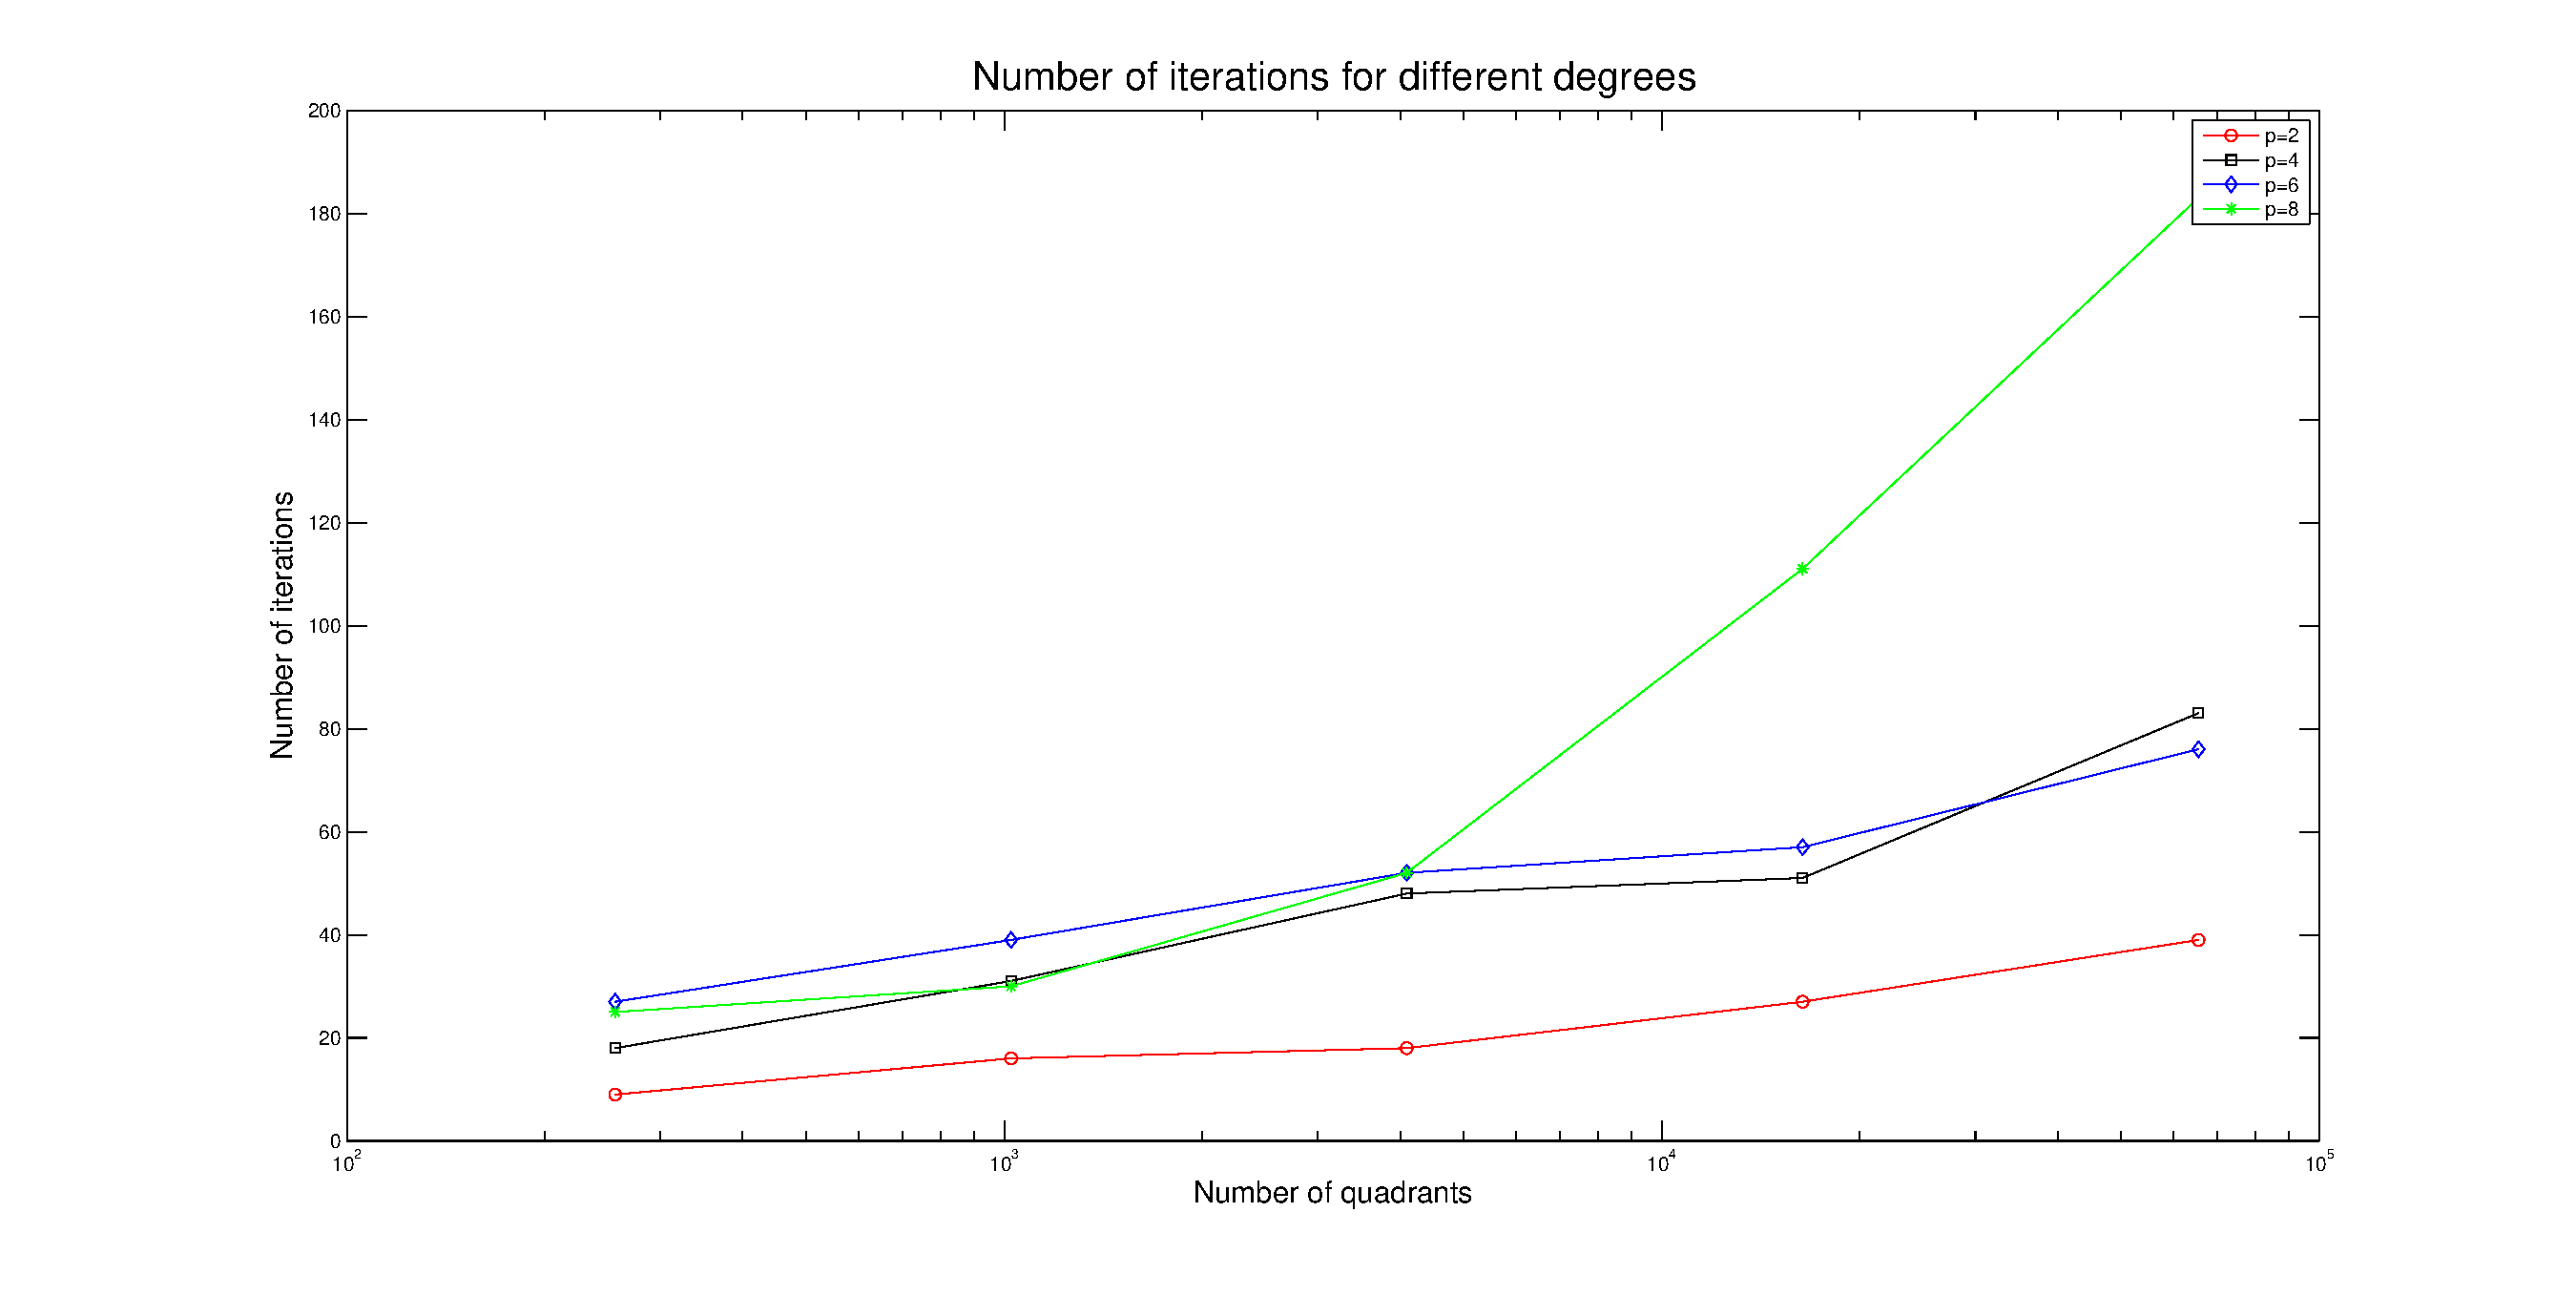
\includegraphics[scale=0.35]{Results/fine_reg_iter.eps}
\caption{Number of iterations of PCG with only the fine preconditioner for different degree $p$ of interpolation as a function of the number of quadrants in a regular mesh.}
\label{fine_reg_iter} 
\end{figure}

We can see that, even without the coarse preconditioner, we are solving the system in a small number of iterations compared to the number of degrees of freedom. For example, we only do about 80 iterations to solve the system with $2.4\: 10^{6}$ degrees of freedom and with interpolations of degree $p=6$. 

 We can also see that for every degree, the number of iterations increases when we refine the mesh. This is to be expected since the information from the boundaries has to go through more quadrant before propagate to the entire domain. Asymptotically, the number of iterations is expected to double as the number of quadrants is multiplied by four (i.e. the mesh size is divided by two). We can see that it is not yet the case here.

A last remark we can make is that the number of iterations tends to increase when the degree of the interpolation increases. This is especially true for the finest mesh where we need 183 iterations for $p=8$ where we only need 39 iterations for $p=2$. This can be explained by the fact that the size of the overlap decreases when $p$ grows. As mentioned in \textcolor{red}{Ref here!!}, this issue would be fixed if we imposed a constant overlap.

\subsubsection{Meshes with distorted elements}
Let us now move on to meshes that are not regular anymore. Let us remember that when we developed the fine preconditioner, we assumed that the elements were rectangular which allowed us to compute the analytic solution to the problem. This part explores the influence of having distorted elements on the number of iterations needed to obtain a given accuracy. 

\begin{figure}
\centering
\begin{subfigure}{.5\textwidth}
  \centering
  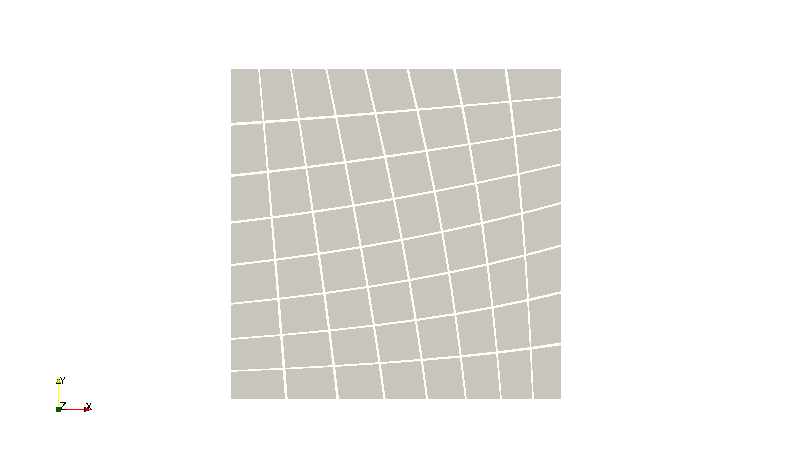
\includegraphics[width=1.2\linewidth]{Results/fine_mesh_deform_1.png}
  \caption{Mesh with $a=1.1$}
  \label{fine_mesh_deform_1}
\end{subfigure}%
\begin{subfigure}{.5\textwidth}
  \centering
  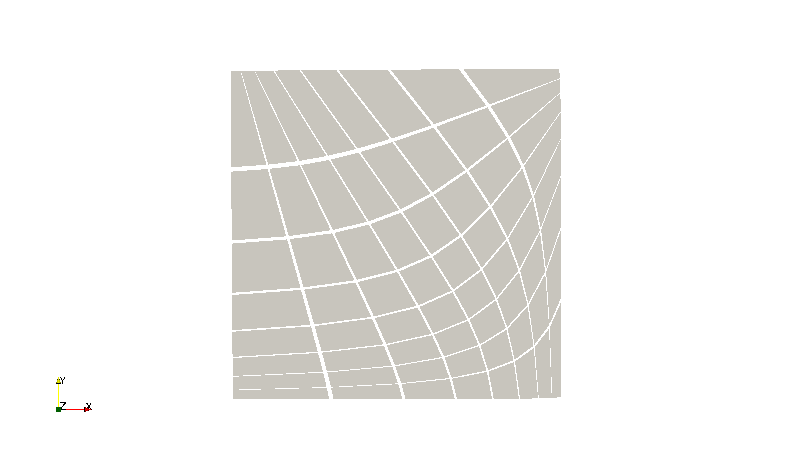
\includegraphics[width=1.2\linewidth]{Results/fine_mesh_deform_2.png}
  \caption{Mesh with $a=1.4$}
  \label{fine_mesh_deform_2}
\end{subfigure}
\caption{Examples of the meshes used for the tests of the fine preconditioner with distorted elements. The meshes are created using GMSH with its progression tool. The key parameter is the common ratio $a$ that we will be increasing progressively.}
\label{fine_mesh_deform}
\end{figure}

To control the deformation, we will continually deform the regular mesh using the progression tool of GMSH \textcolor{red}{ref here!!}. The deformation is performed using a geometric progression, using the common ratio $a$ as the parameter. Obviously, the higher the parameter $a$, the more distorted the mesh is. It is clear that for $a=1$, we have a regular mesh. Figure \ref{fine_mesh_deform} presents three meshes of obtained with the progression with GMSH. On the left we used $a = 1.1$ and on the right we used $a=1.4$. 

Using the same tolerance as in the previous part, we ran the preconditioned conjugate gradients with the fine preconditioner for those new meshes. The order of the interpolation used is $p=2$. The results are given in figure \ref{fine_dist_iter}.

We can see, as it was expected, that the more we deform the mesh, the more iterations we need to do in order to obtain the wanted accuracy. The fact that, for distorted elements, we do not invert exactly the system but use an approximation allows us to compute the fine preconditioner efficiently even when we have a lot of elements but we can see here that it also costs more iterations of the preconditioned conjugate gradients. However, the gain is still huge. Indeed, for a degree of interpolation $p$, we have $(p+3)^2$ nodes per overlapping subdomain. This means a complexity of $\mathcal{O}((p+3)^6)$ to solve the system exactly. Instead, with the method we use, the only need to do a few matrix multiplications where the matrices have $(p+3)$ rows and columns. This means a complexity of $\mathcal{O}((p+3)^2)$. Even with $p=2$, the results shows that it is much faster to not take geometric factors into account. 

We can also note that the effect of increasing the number of elements (i.e. reducing the mesh size) on the number of iterations is clearer here. For example, for the mesh with $a = 1.15$, we need 10 iterations for $8^2$ elements, 18 iterations for $16^2$ elements and 39 iterations for $32^2$ elements. The same explanation applies here : when we multiply the number of elements by four, we roughly multiply the number of quadrants in each direction by two and therefore the information needs twice as many iterations to propagate to the domain. 

\begin{figure}
\centering
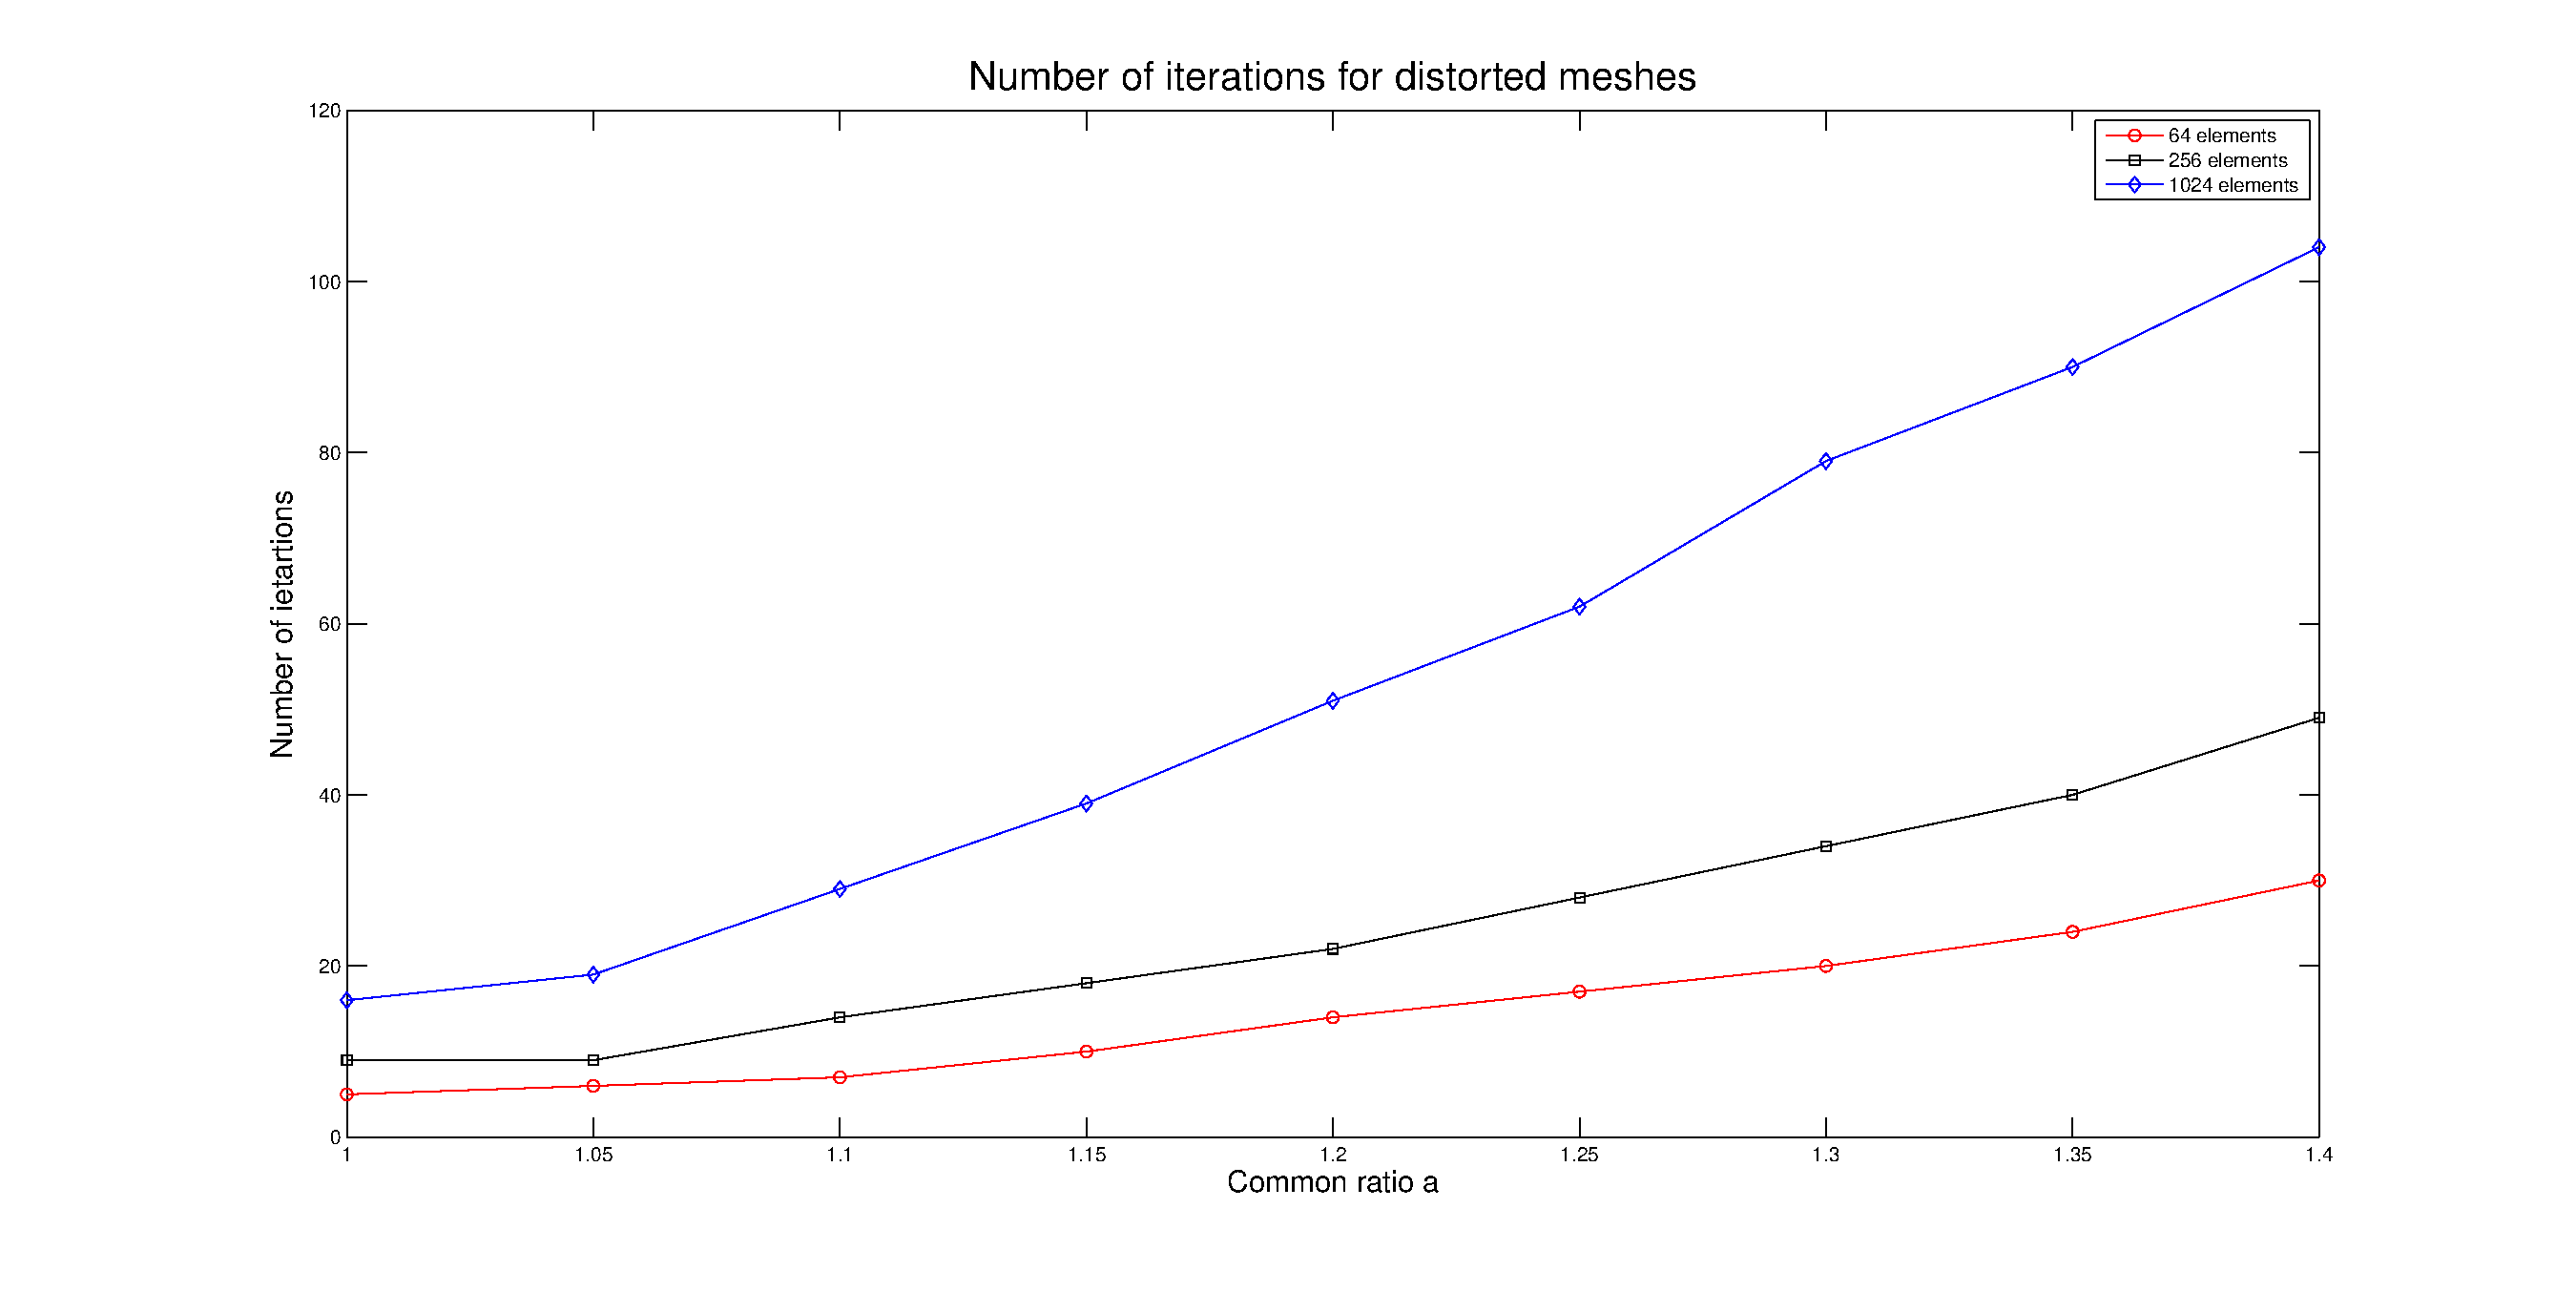
\includegraphics[scale=0.35]{Results/fine_dist_iter.eps}
\caption{bla}
\label{fine_dist_iter}
\end{figure}



\subsection{Influence of hanging nodes}
 In this part, we will explore the influence of hanging nodes on the number of iterations needed by the preconditioned conjugate gradients with the fine preconditioner to converge. Because we want meshes that are not artificial and come from real AMR applications, we will change the forcing term in this part and we will also use a recursive refine function when we build the mesh with p4est. 
 
 Let us first define the problem and the forcing term. As before, the domain is : $\Omega = [-1;1]^2$ and $\Gamma$ is the boundary. We will solve : 
 
 \begin{align}
 \nabla^2 u &= -2\tanh(nx)\tanh(my)\left[ n^2(1-\tanh(nx)^2) + m^2(1-\tanh(my)^2)\right] &\text{on $\Omega$} \label{eq:prob3}\\
u &= \tanh(nx)\tanh(my)  &\text{on $\Gamma$}
 \end{align}
 
 We can see that problem \ref{eq:prob3} has an analytic solution that is given by :
 
 $$u(x,y) = \tanh(nx)\tanh(my)$$
 
 The parameters $n$ and $m$ can be adjusted to make the jump in the hyperbolic tangent more steep. An example of a numerical solution with $p=1$ and obtained by our multigrid solver has already been shown on figure \ref{multi_simple_sol} for $n=3$ and $m=3$. 
 
 As explained before, we will use a recursive refine function when we build the forest. Since we know the analytic solution, we can cheat a little and use it for the refinement process. We will ask that the absolute value of the difference between the value of $u$ in the center of the quadrant and the mean of the values of $u$ at the four corners of the quadrant is less than a fixed tolerance multiplied by the maximum value of the function. So, if the four corners have coordinates $(x_i , y_i)$ for $i=0,1,2,3$, and that $u_{max} = max_{x,y \in \Omega} \left| u \right|$, we impose the following rule :
 
\begin{align}  
  \left| u(\frac{1}{4}\sum_{i=0}^3 x_i , \frac{1}{4}\sum_{i=0}^3 y_i) - \frac{1}{4}\sum_{i=0}^3 u(x_i,y_i) < u_{max} tol\right|
  \label{hang_rel}
\end{align}
  
Where $tol$ is a fixed tolerance. Intuitively, the tighter the tolerance, the more refined the grid needs to be and the more hanging nodes we will have thanks to the jump in the hyperbolic tangent function. 

\subsubsection{Increasing the relative number of hanging nodes}

To have a rather steep jump, we chose $n=m=12$ for the different tests that follow. We varied the tolerance to have more or less hanging nodes. We also needed a way to quantify the presence of hanging nodes. Let us define $hang$, the ratio of the number of hanging nodes over the number of global nodes. 

\begin{align}
 hang = \frac{\#\text{hanging nodes}}{\#\text{global nodes}}
 \label{hang_frac}
 \end{align}

\begin{table}
\centering
\begin{tabular}{c|ccc}
\hline
Tol & 0.020 & 0.015 & 0.010\\
\hline
Number of quadrants &1276 & 1384 & 3064 \\
\hline
hang & 14.05\% & 16.61\% & 22.13\%\\
\hline
\end{tabular}
\caption{Number of quadrants obtained using the recursive refine function on the problem \ref{eq:prob3} for different tolerances as well as the ratio $hang$ for each mesh with an interpolation of degree $p=2$.}
\label{fine_hanging_ratio}
\end{table}

Table \ref{fine_hanging_ratio} shows this number for different values of the tolerance and for $p=2$. We can see, as expected, that the ratio $hang$ increases while we make the tolerance tighter. Of course, the exact value of $hang$ does not matter since even for a given mesh, it will change with the degree of the interpolation so it is rather how it evolves that interests us. 

\begin{figure}
\centering
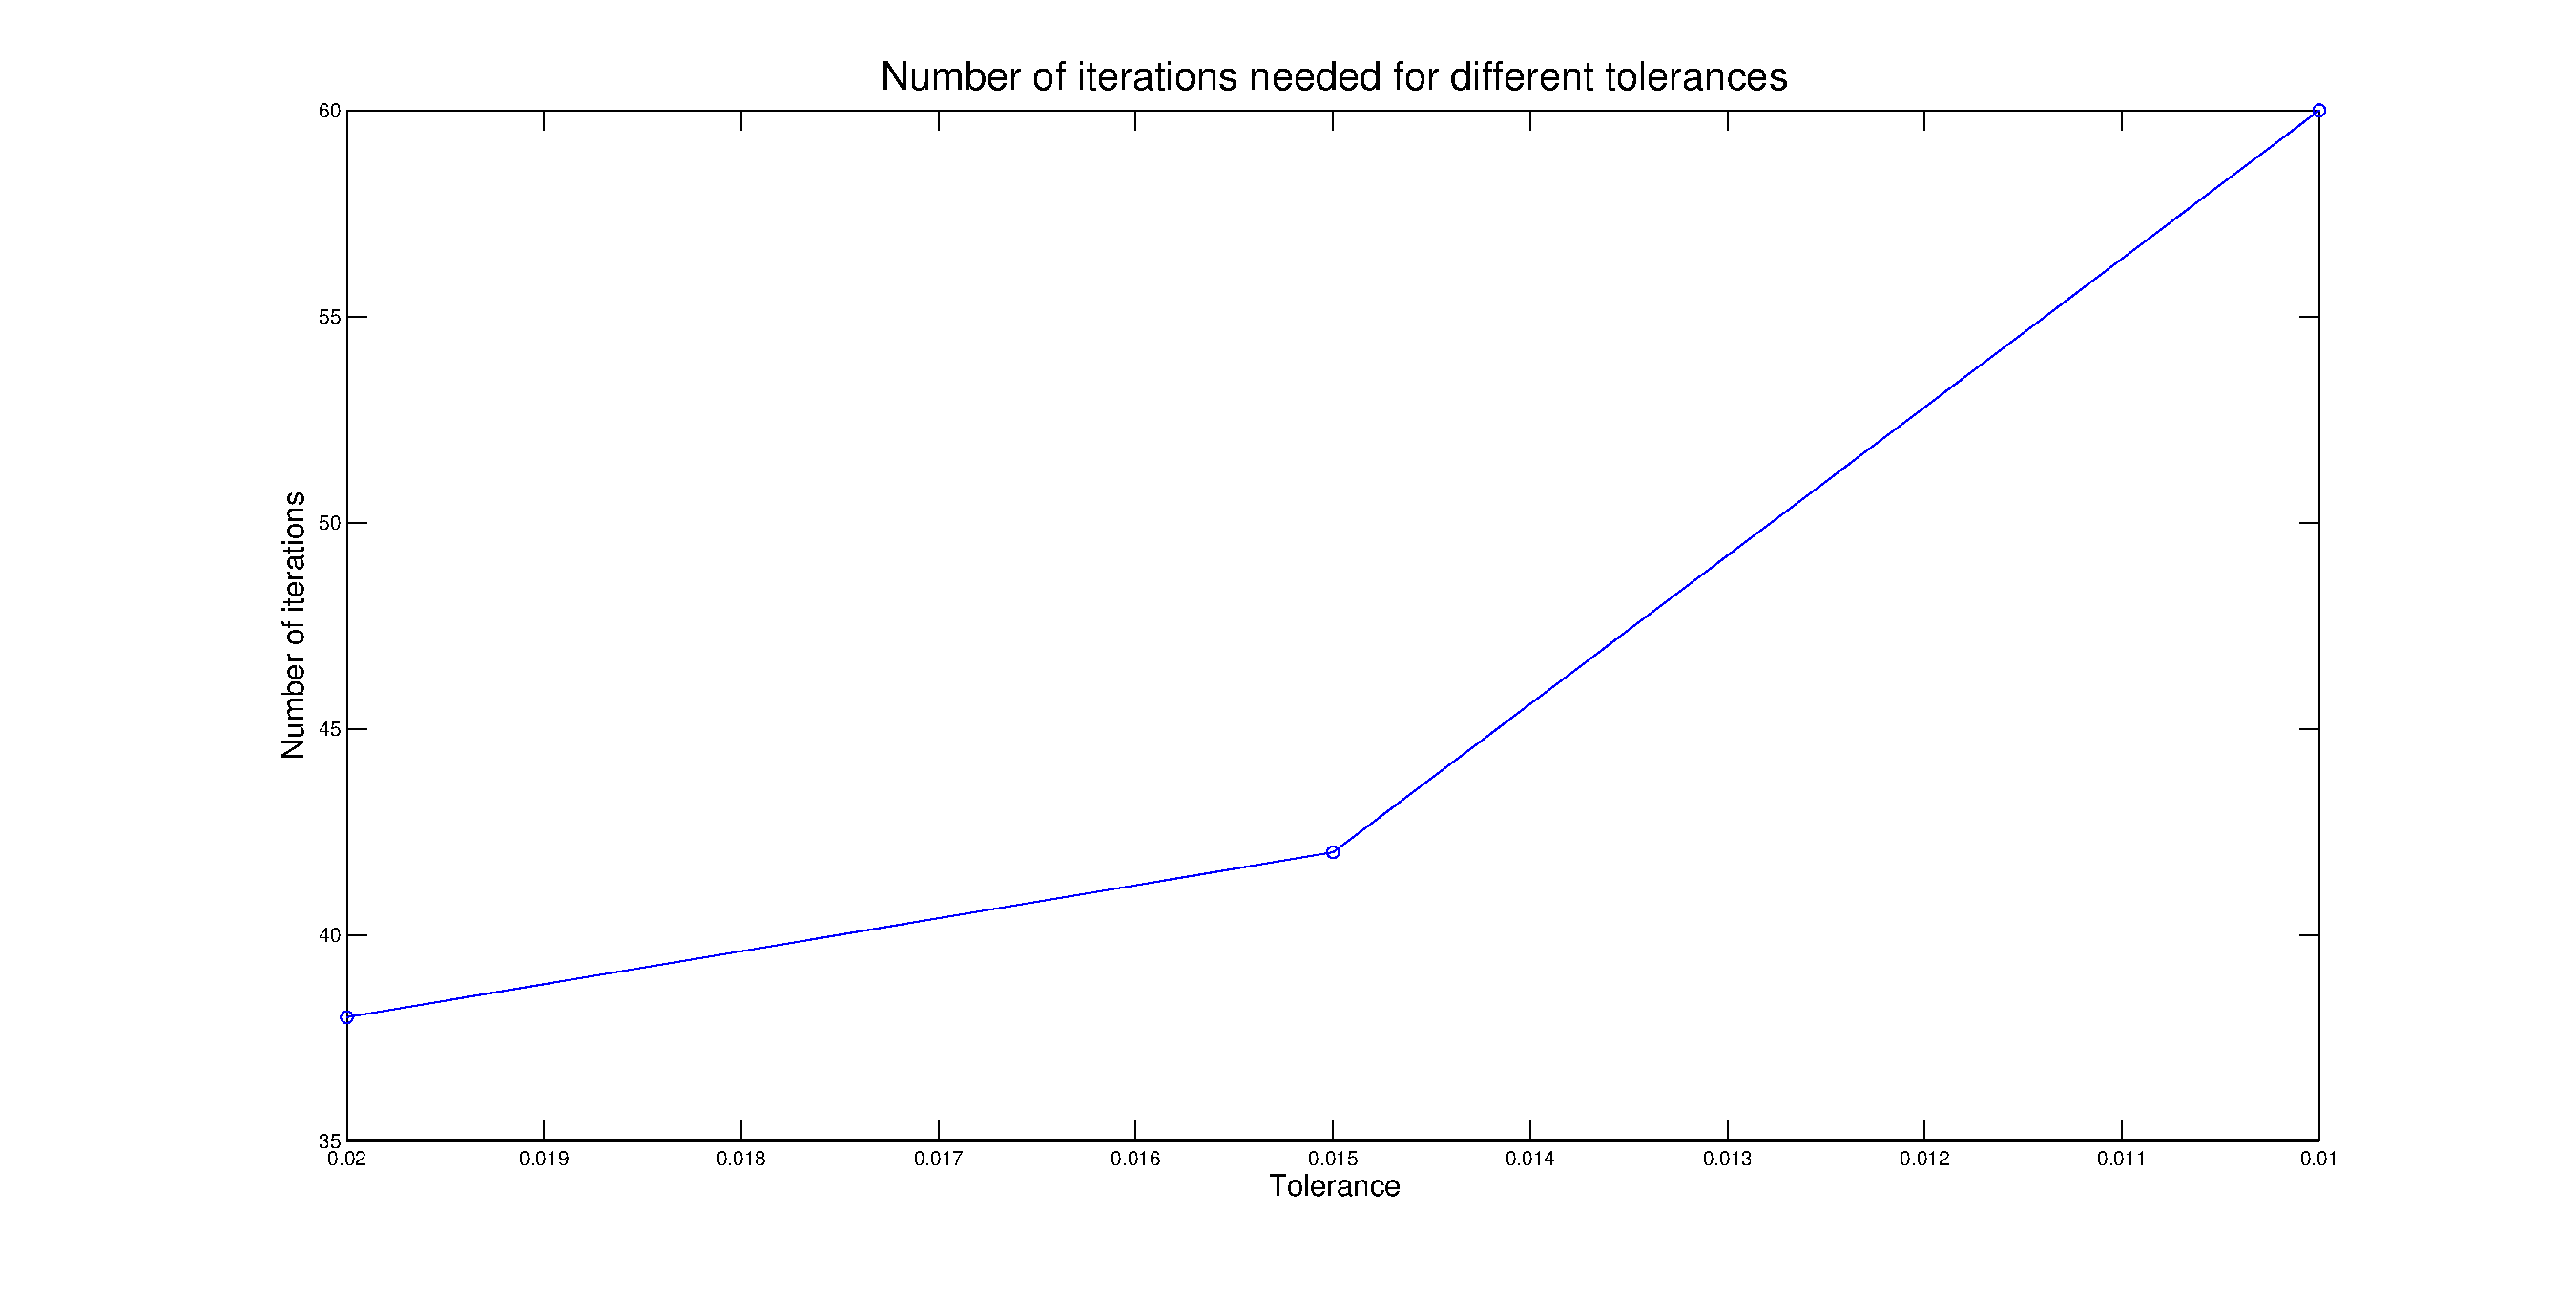
\includegraphics[scale=0.35]{Results/fine_hang_plot.eps}
\caption{Number of iterations needed to reach a given norm on the residual for a degree of interpolation $p=2$ and for meshes obtained with different tolerances.}
\label{fine_hang_plot}
\end{figure}


Let us now see how the number of iterations varies for the different meshes. Figure \ref{fine_hang_plot} shows the number of iterations needed to reach the same norm on the residual as before for the three different meshes obtained with the tolerances presented in table \ref{fine_hanging_ratio}. We can see on the graph that the number of iterations increases when we have relatively more hanging nodes. We have to be careful since this phenomenon can also be explained by the fact that we have more quadrants when the tolerance gets tighter and that also causes an increase in the number of iterations as showed earlier in this section. However, it is observed that we need less iterations when we do not have hanging nodes and for a similar number of quadrants (for example, for 1024 quadrants without hanging nodes, we need 18 iterations whereas we need 38 for 1276 quadrants). 


As explained in the theory chapter, when we have hanging nodes, we do not treat all hanging possibilities and therefore we have an error when we compute the local residual. This explains why we need more iterations in presence of hanging nodes and the fact that we converge less quickly the more hanging nodes we have in the mesh. However, the number of iterations is still acceptable.

\subsubsection{Increasing the degree of the interpolation} 

\begin{figure}
\centering
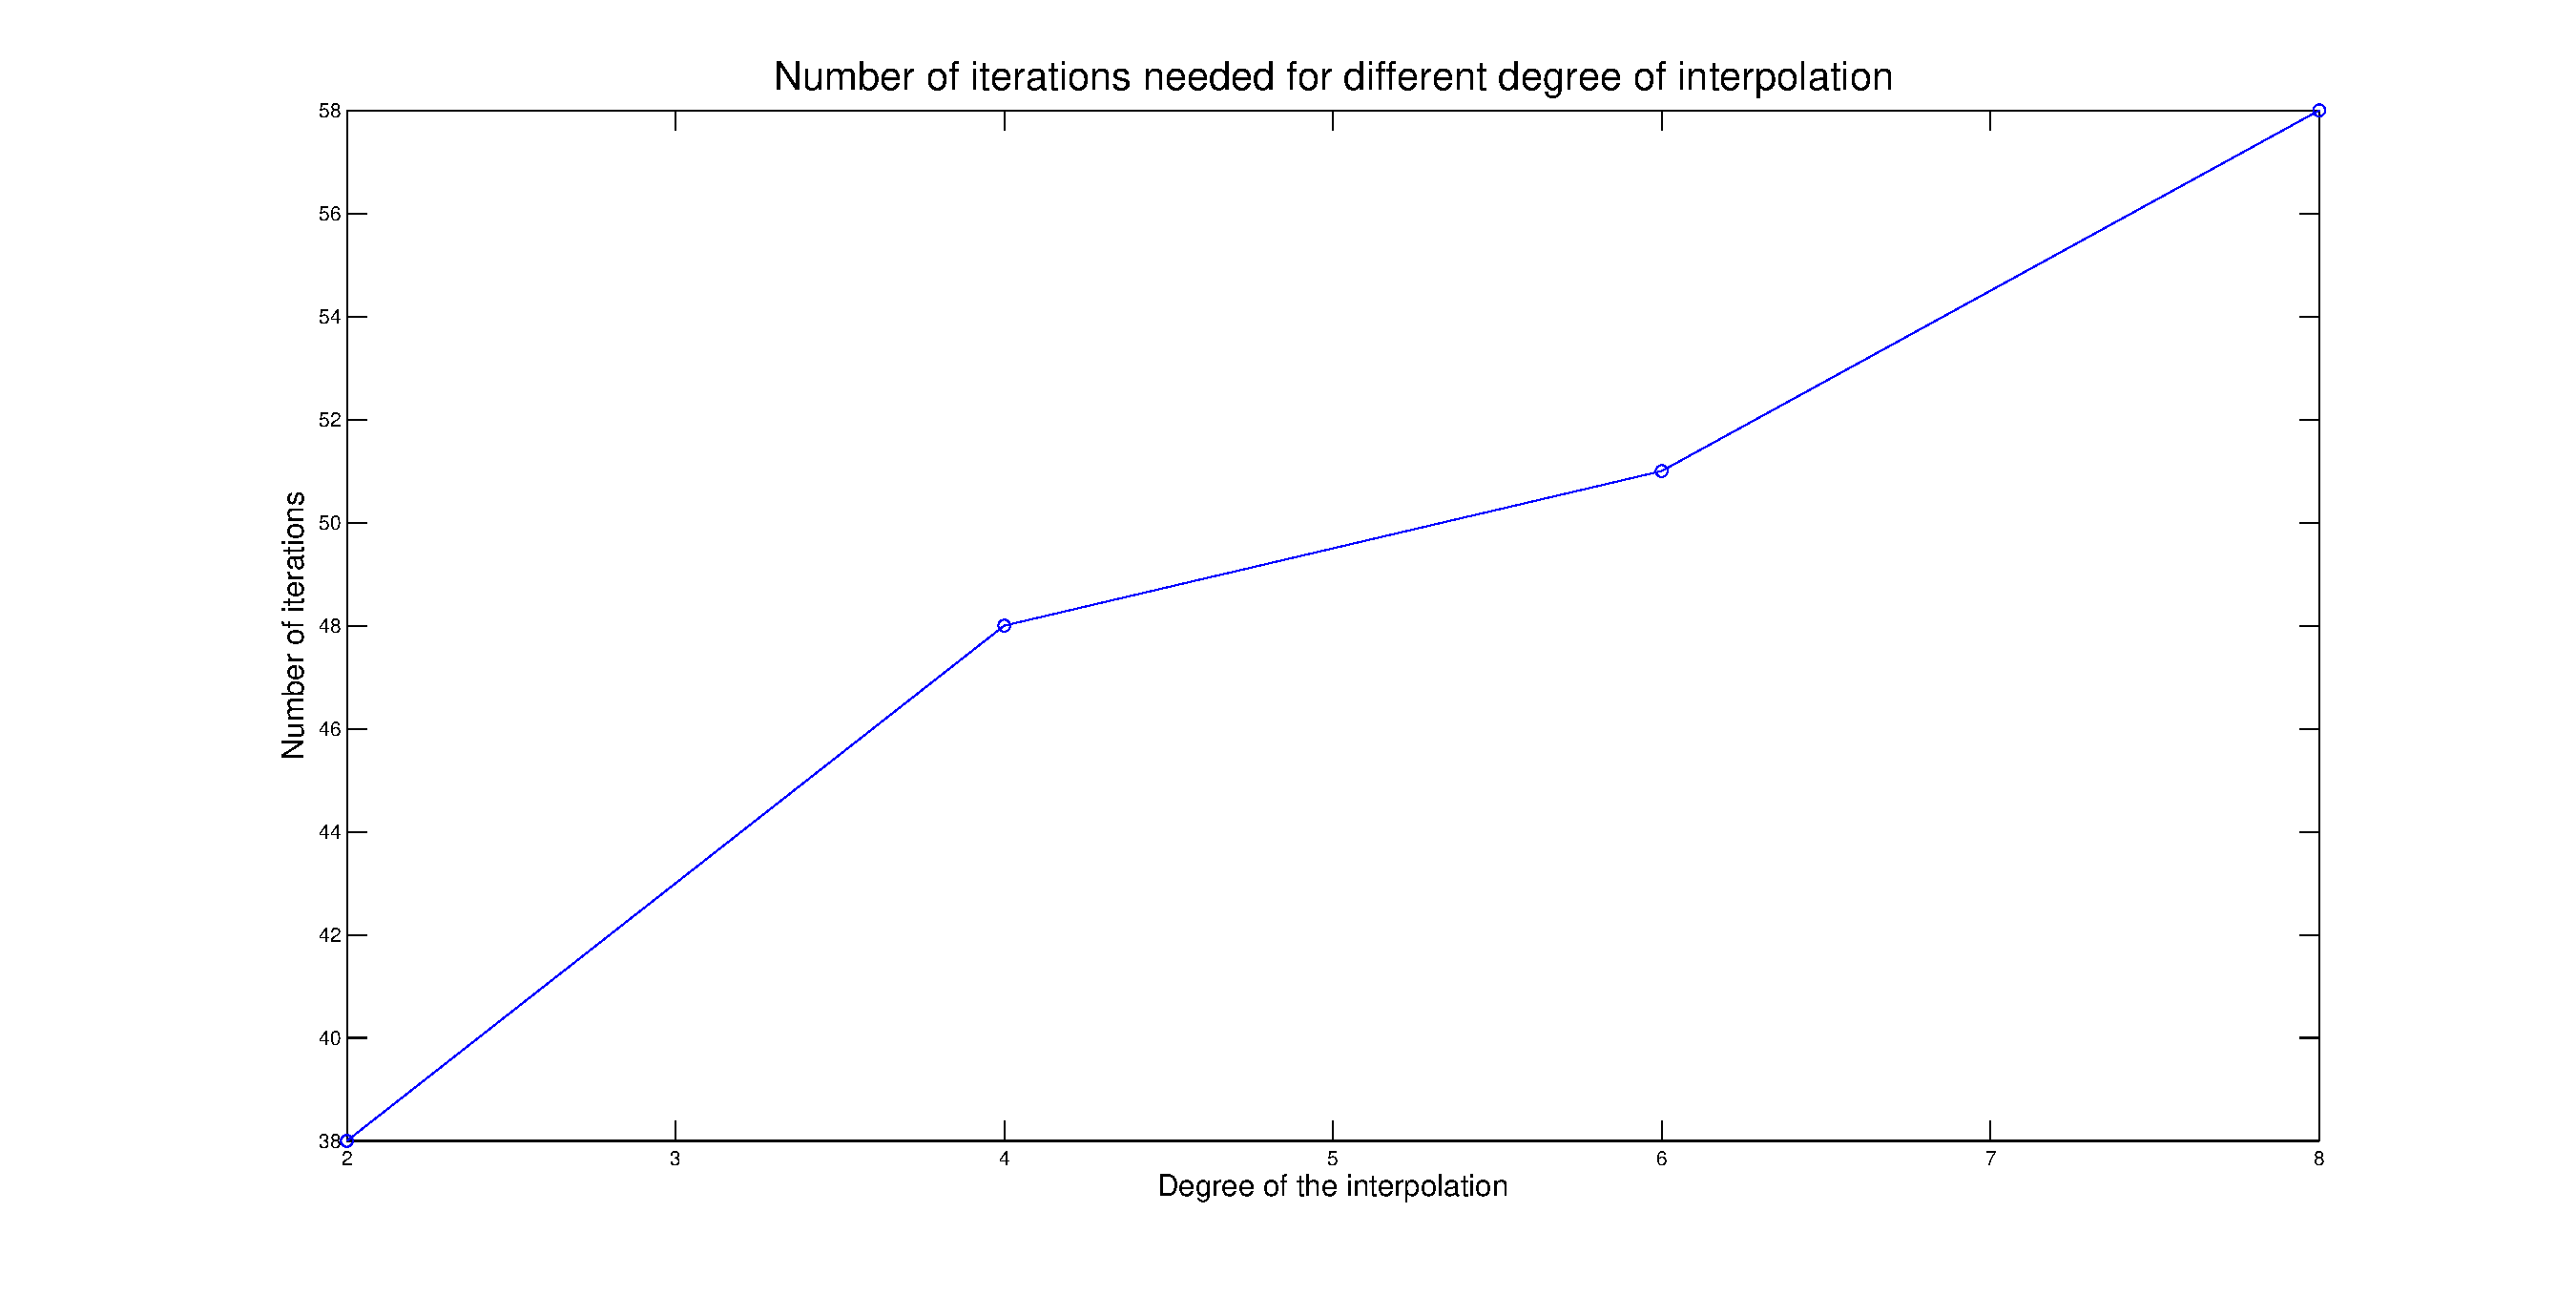
\includegraphics[scale=0.35]{Results/fine_hang_deg.eps}
\caption{Number of iterations needed to reach the tolerance of the norm of the residual as a function of the degree of the interpolation used for a mesh obtained using $tol=0.02$ in the recursive refine function.}
\label{fine_hang_deg}
\end{figure}

Let us finally look at what happens when we increase the degree of the interpolation. We tried different degrees of interpolation ($p=2,4,6,8$) and look at the number of iterations needed to obtain the numerical solution. Figure \ref{fine_hang_deg} shows the results.  

We can see that the number of iterations increases with the degree. We need 38 iterations for $p=2$ but 58 for $p=8$. As already explained in the case with no hanging nodes, this is in part due to the fact that when we increase the degree of the interpolation, the size of the overlap decreases and therefore we need more iterations.

We can also mention the fact that since we do not treat all hanging possibilities when we compute the local residual at the overlaps, increasing the degree (and therefore the number of nodes in the overlaps) might have a effect on the number of iterations.

All the tests presented here were on meshes where the elements were not distorted and where we expect the fine preconditioner to behave optimally but the same tests have been performed with distorted quadrants and we observe the same qualitative results. 


 



 

\section{Two scale preconditioner}

Let us finally move on to the two-scale preconditioner. We showed in the previous part that using only the fine scale preconditioner was not a good idea when the number of quadrants increased (the number of iterations roughly doubles when the mesh size is divided by two). As explained in the theory chapter, the idea is to add a coarse part in the preconditioner (i.e. $P = P^f + P^c$), consisting mainly of solving a problem with an interpolation degree $p=1$ with a geometric multigrid method, so that the number of iterations stays constant when we increase the number of quadrants.  

As in the previous section, the tests will be performed in two parts : first, we will analyze the performances of the two-scale preconditioner when there are no hanging nodes (but for both regular and distorted meshes) and then we will look at what happens when the forest of quadtrees is refined recursively and therefore the mesh is not conforming anymore. 

In the last subsection, we will also motivate the choice of using higher order degrees of interpolation. We will indeed look at the best degree to obtain a given accuracy in the solution, i.e. the degree for which we have the solution to a given problem on a given mesh in the shortest amount of time and that is accurate enough. 

\subsection{No hanging nodes}

Let us first present the problem we will solve in this part. We want our numerical solution to capture both low and high frequency modes so we will superpose a cosine with low frequency and a sine with a high frequency. As before, the domain is : $\Omega = \left[ -1;1 \right]^2$ and $\Gamma$ is the boundary. We will solve : 

\begin{align}
\nabla^2 u &= -\frac{\pi^2}{2}\cos(\frac{\pi}{2}x)\cos(\frac{\pi}{2}y) - 5\pi^2\sin(5\pi x)\sin(5\pi y) &\text{on $\Omega$} \label{eq:prob_two}\\
u &= 0  &\text{on $\Gamma$}
\end{align}

This problem has an analytic solution that is given by : 

$$ u(x,y) = \cos(\frac{\pi}{2}x)\cos(\frac{\pi}{2}y) + \frac{1}{10}\sin(5\pi x)\sin(5\pi y)$$

\begin{figure}
\centering
\includegraphics[scale=0.35]{Results/two_simple_sol.eps}
\caption{Numerical solution to problem \ref{eq:prob_two} using an interpolation of order $p=2$ and $1.0\:10^{6}$ degrees of freedom on a regular mesh with no hanging nodes. This numerical solution has been obtained by the PCG with the two scale preconditioner.}
\label{two_simple_sol}
\end{figure}


An example of a numerical solution obtained using the preconditioned conjugate gradients with the two scale preconditioner can be seen on figure \ref{two_simple_sol}. This solution has been obtained in only 8 iterations and with an interpolation of degree $p=2$. 

\subsubsection{Regular meshes}

Let us now look at what happens to the number of iterations when we decrease the mesh size for different degrees of interpolation. Table \ref{two_table_reg} shows the number of degrees of freedom for the different meshes used (indeed, for a given mesh, the higher the degree of the interpolation, the more global nodes we have). We can already see that, thanks to the coarse preconditioner, we are able to have a lot more degrees of freedom than in the case where we only had the fine preconditioner.

\begin{table}
\centering
\begin{tabular}{c|cccc}
\hline
Number of quadrants & $128^2$ & $256^2$ & $512^2$ & $1024^2$\\
\hline
$p=2$ & $6.6\:10^4$ & $2.6\:10^5$ & $1.1\:10^6$ & $4.2\:10^6$ \\
$p=4$ & $2.6\:10^5$ & $1.1\:10^6$ & $4.2\:10^6$ & $1.7\:10^7$ \\
$p=6$ & $5.9\:10^5$ & $2.4\:10^6$ & $9.4\:10^6$ & $3.8\:10^7$ \\
$p=8$ & $1.1\:10^6$ & $4.2\:10^6$ & $1.7\:10^7$ & $6.7\:10^7$ \\
\hline
\end{tabular}
\caption{Number of degrees of freedom for a regular mesh with different numbers of quadrants and for different degrees of interpolation.}
\label{two_table_reg}
\end{table}

\begin{figure}
\centering
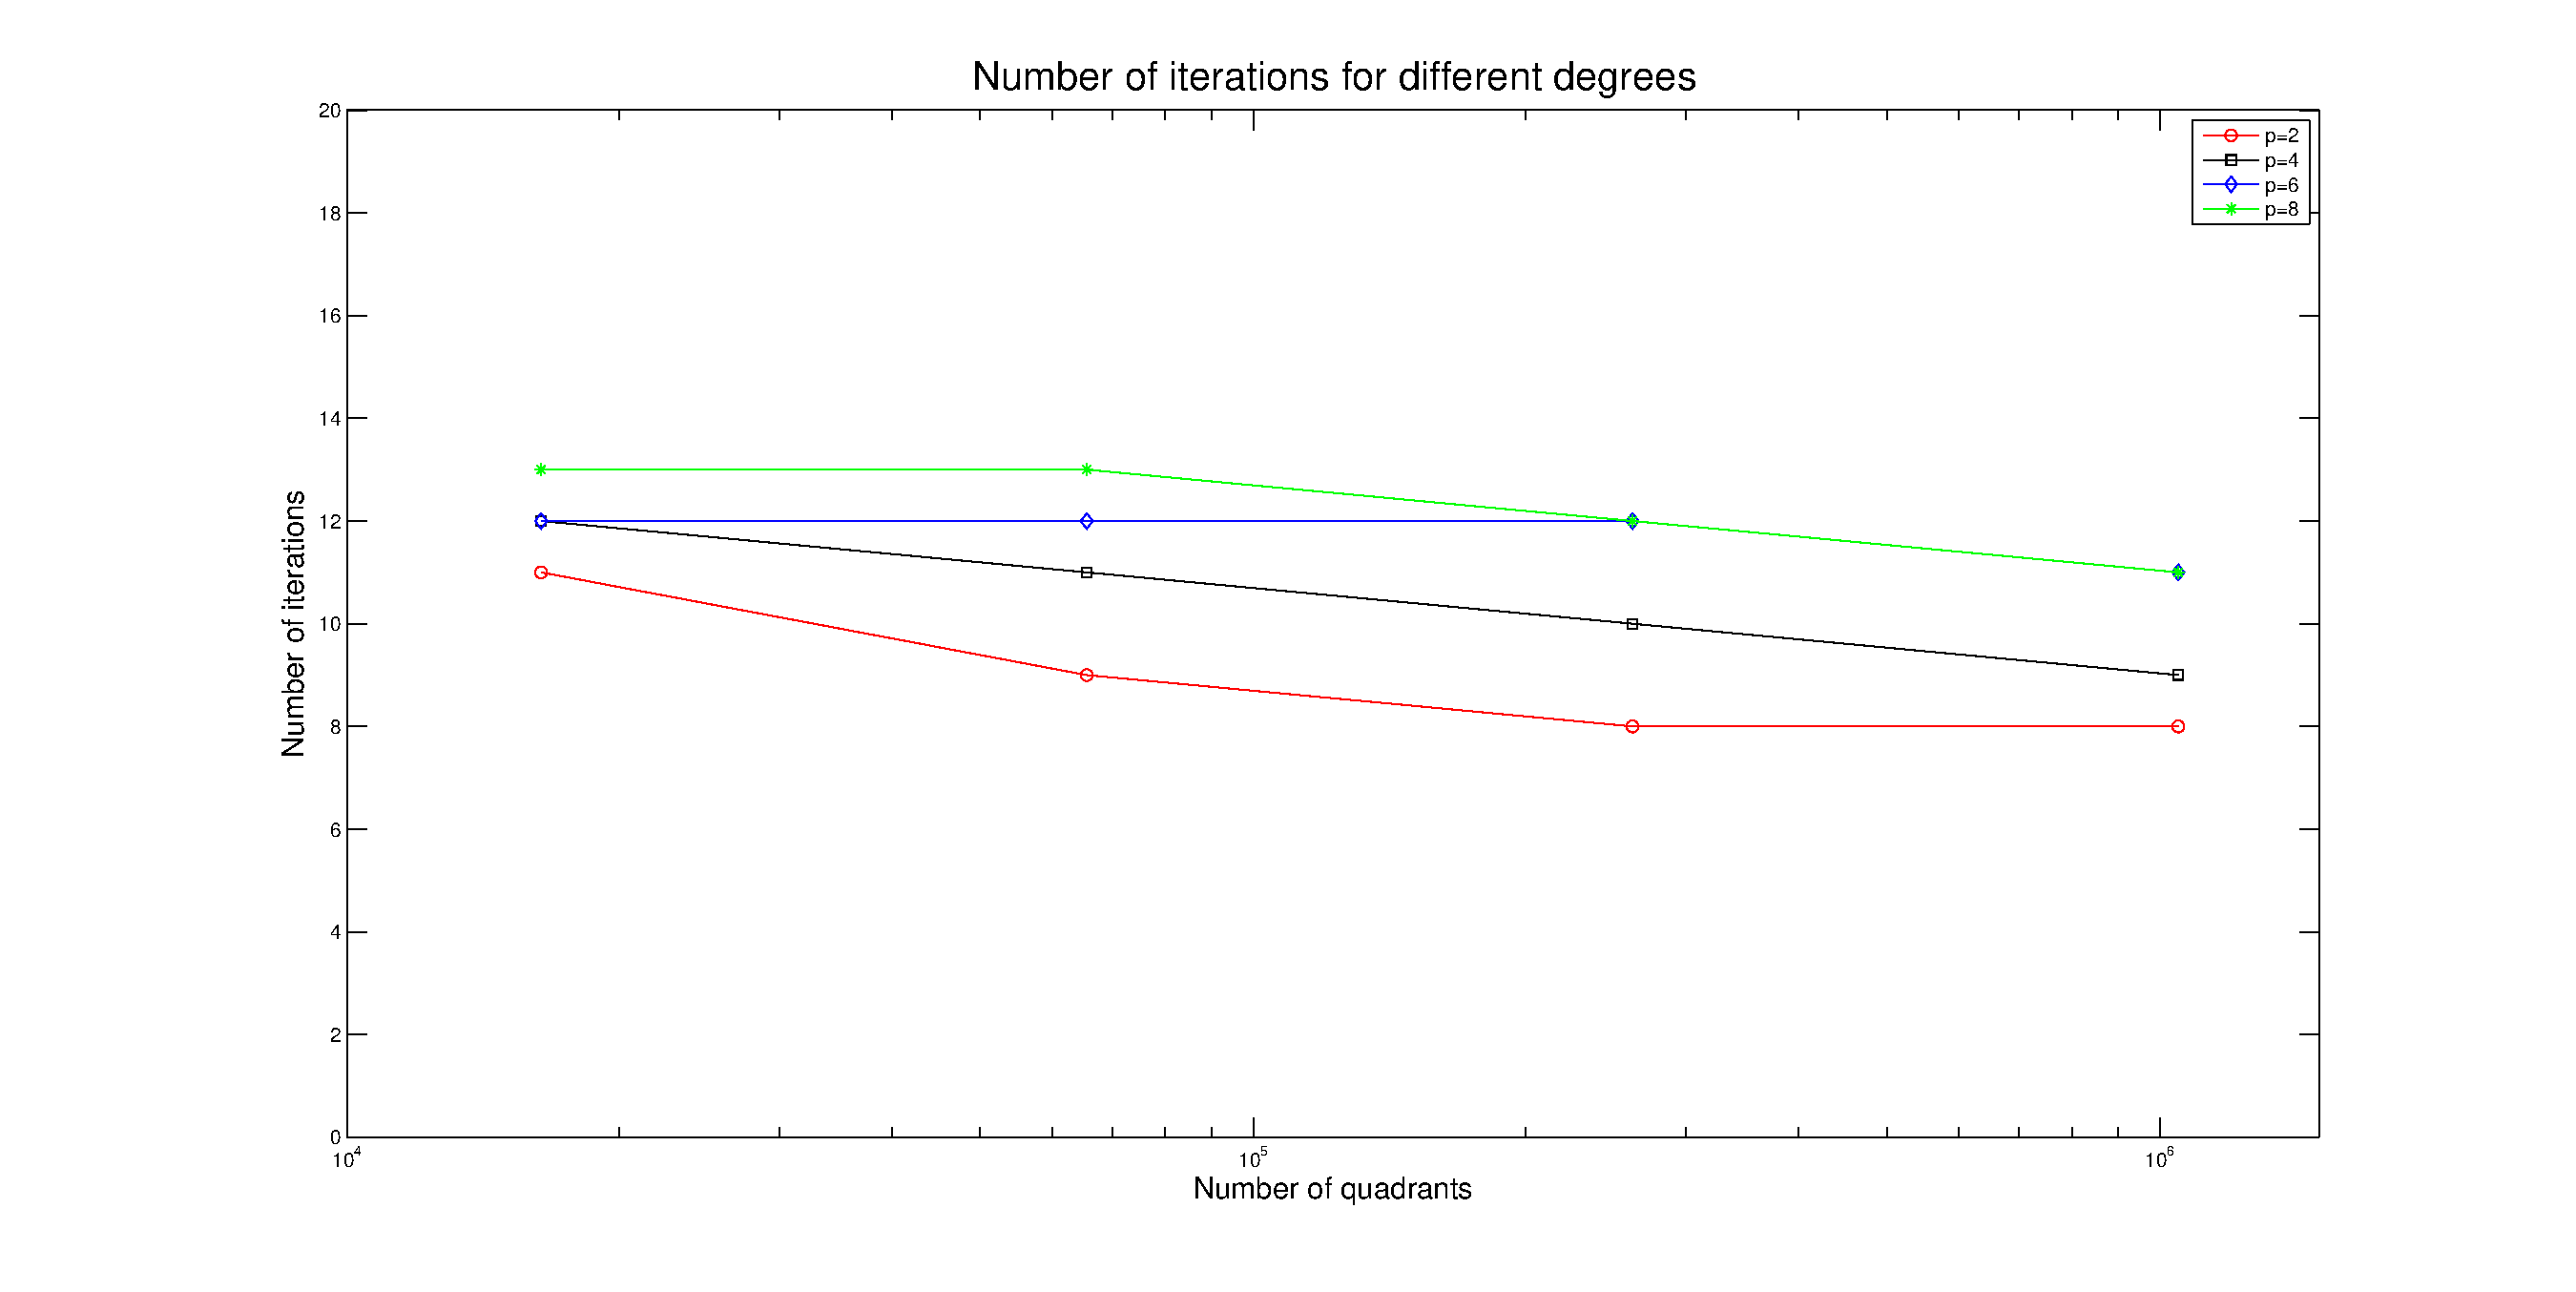
\includegraphics[scale=0.35]{Results/two_reg_iter.eps}
\caption{Number of iterations of PCG with the two scale preconditioner for degree $p$ of interpolation needed to reach the given tolerance of the norm of the residual as a function of the number of quadrants in a regular mesh.}
\label{two_reg_iter}
\end{figure}

For the following tests, we also have tighten the tolerance on the norm of the residual. We now require that : 

$$\frac{||r_k||_2}{||r_0||_2} < 10^{-5}$$

Figure \ref{two_reg_iter} shows the number of iterations needed to reach that tolerance of the norm of the residual when we use our two scale preconditioner for different degrees of interpolation. The first remark we can make is that the number of iterations does not increase with the number of quadrants (as it was the case when we only had the fine preconditioner). So we can conclude that the coarse preconditioner does the job it was designed to do. We can even note that the number of iterations slightly decreases. For example, for $p=6$, we need 12 iterations for $128^2$ quadrants but we only do 11 iterations for $1024^2$. An explanation for this phenomenon might be that when we increase the number of quadrants, we actually better separate the actions of the fine and coarse preconditioners and therefore the sum of the two is a better approximation of $A^{-1}$. We can mention that for $p=8$, we only need 11 iterations to solve a system that has more than 67 millions unknowns. 

A second remark we can make, as already observed when we only had the fine preconditioner, is that the number of iterations grows with the degree of the interpolation. For example, with $1024^2$ quadrants, we need 8 iterations when $p=2$ but we need to do 11 iterations when $p=8$. As before, this can be explained by the fact that as the degree of the interpolation increases, the size of the overlap decreases. A fixed sized overlap would fix this issue. 

\subsubsection{Meshes with distorted elements}

We will now look at what happens when the mesh is not regular but we have quadrants that are more and more distorted. We will use the same meshes already used in the previous section and obtained with the progression tool of GMSH (see figure \ref{fine_mesh_deform} for example of such meshes).

\begin{figure}
\centering
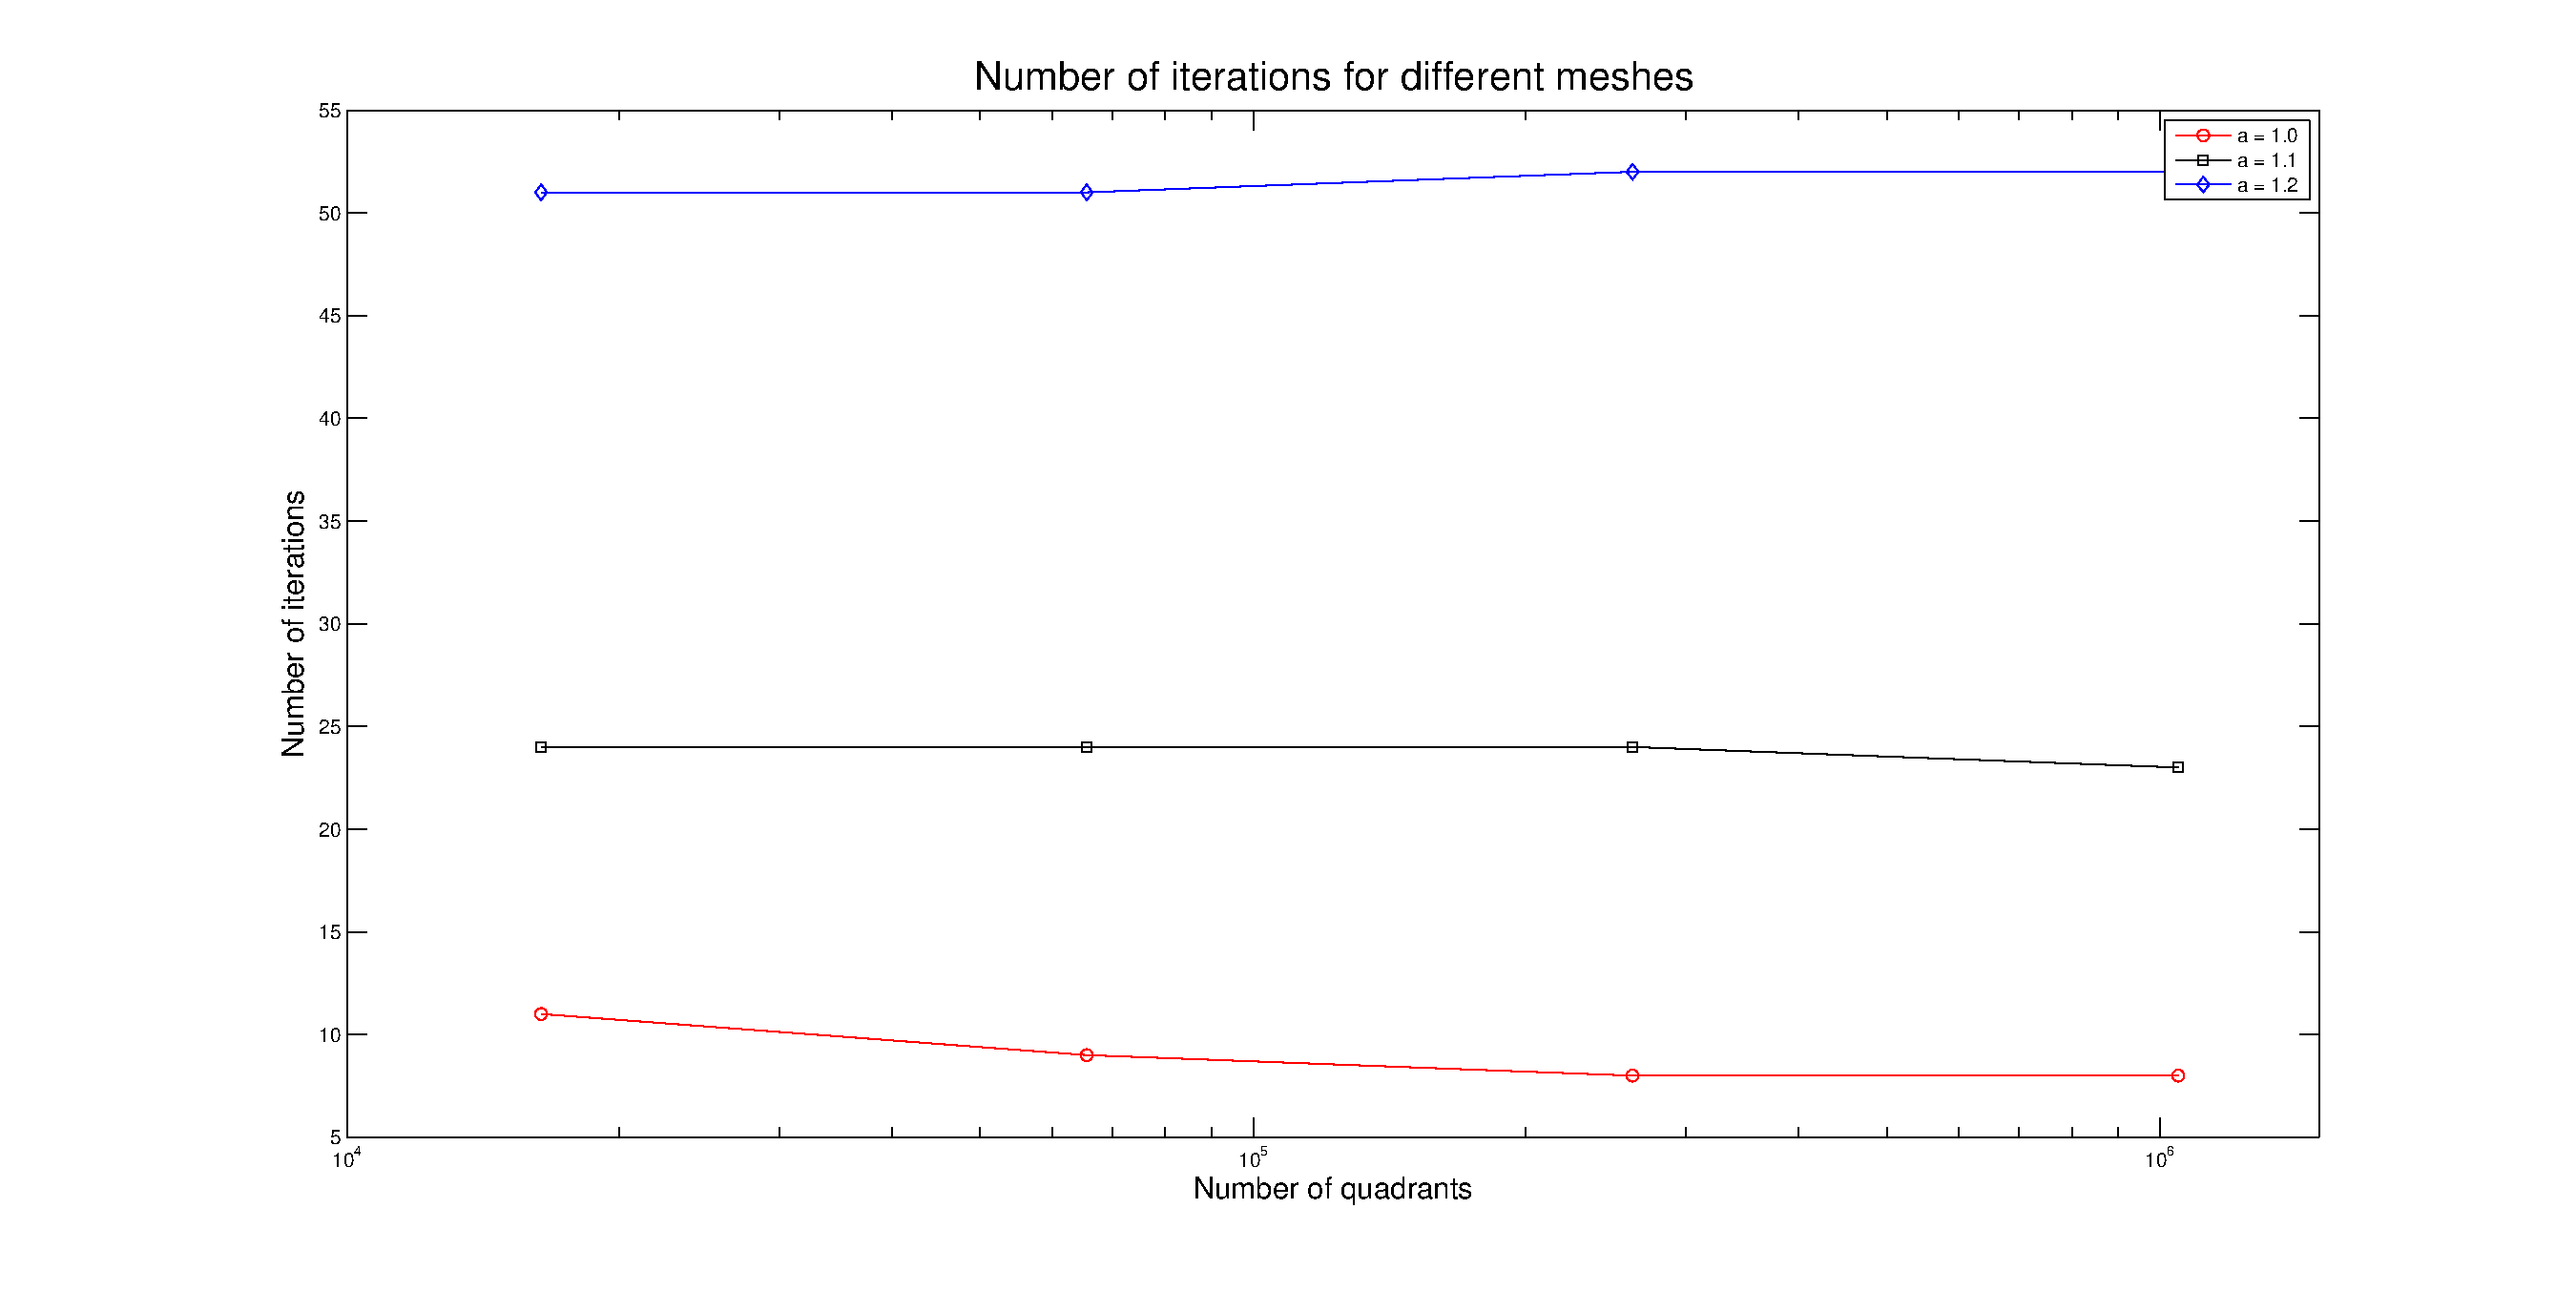
\includegraphics[scale=0.35]{Results/two_irreg_iter.eps}
\caption{Number of iterations of PCG with the two scale preconditioner for an interpolation degree $p=2$ needed to reach the given tolerance on the norm of the residual as a function of the number of quadrants for meshes with quadrants more and more distorted.}
\label{two_irreg_iter}
\end{figure}

For an interpolation of degree $p=2$, we looked at the number of iterations needed to reach the given tolerance as we increased the number of quadrants and for elements more and more distorted. Figure \ref{two_irreg_iter} shows the results. We can see that the number of iterations stays roughly the same when we increase the number of quadrants so once again the coarse part of the preconditioner does the job it is designed to do. 

We can also node that the more we distort the quadrants the more iterations we need to reach the given tolerance. This is to be expected since we developed the fine preconditioner to work optimally on quadrants aligned with the axis. This means that the more a quadrant is distorted the less accurate is the fine preconditioner part and therefore the more iterations we need. However, even with the most distorted mesh, the number of iterations stays acceptable and as explained in the previous section, the gain of not having to solve exactly on every quadrant is huge. We also have to say that the meshes presented here have an intrinsic structure since they are generated using the progression tool in GMSH. Therefore, the errors we make with our approximation are always in the same direction and the number of iterations needed increases. We might not have such an increase with a random mesh containing quadrants with the same quality measure. 


\subsection{Influence of hanging nodes}

Let us now move on to the cases where we have hanging nodes. As in the part with only the fine preconditioner, we will look at a problem where the solution has a jump so that we create hanging nodes when we use a recursive refine function in p4est. In addition to the hyperbolic tangent already presented in the previous subsection, we will include a high frequency sine wave to see how the grid adapts to capture it and how the two scale preconditioner performs in its presence. 

The problem we will solve is : 

\begin{align}
\nabla^2 u =& -2\tanh(12x)\tanh(12y)\left[ 12^2(1-\tanh(12x)^2) + 12^2(1-\tanh(12y)^2)\right] \nonumber \\
 &-  10\pi^2\sin(10\pi x)\sin(10\pi y) &\text{on $\Omega$} \label{eq:two_hang}\\
u =&   \tanh(12x)\tanh(12y) + \frac{1}{20}\sin(10\pi x)\sin(10\pi y)&\text{on $\Gamma$}
\end{align}

Where $\Omega = [-1;1]^2$ and $\Gamma$ is the boundary. This problem has an analytic solution that is given by : 

$$u(x,y) = \tanh(12x)\tanh(12y) + \frac{1}{20}\sin(10\pi x)\sin(10\pi y)$$

\begin{figure}
\centering
\includegraphics[scale=0.35]{Results/two_hang_plot.eps}
\caption{Numerical solution to problem \ref{eq:two_hang} using an interpolation of order $p=2$ on a non conforming mesh and obtained with PCG with the two scale preconditioner.}
\label{two_hang_plot}
\end{figure}

Figure \ref{two_hang_plot} shows an example of the numerical solution computed on a non conforming mesh with PCG and the two scale preconditioner. We can see on the plot both the steep jump due to the hyperbolic tangent and the small oscillations due to the sine wave.

\subsubsection{Increasing the relative number of hanging nodes}

Let us now look at the influence of increasing the number of hanging nodes in the mesh. To achieve this, we will use the same rule in the recursive refinement of the quadrants as in the previous section, given by relation \ref{hang_rel}. We will also tighten the parameter $tol$ used in order to have more quadrants than in the case when we only had the fine preconditioner. 

\begin{table}
\centering
\begin{tabular}{c|ccccccc}
Parameter $tol$ & 0.01 & 0.008 & 0.006 & 0.004 & 0.002 & 0.001 & 0.0005\\
\hline
Number of hanging nodes & 6080 & 8064 & 11008 & 14272 & 23200 & 33696 & 70112\\
Number of global nodes & 19921 & 25545 & 32265 & 49265 & 120201 & 208137 & 445425\\
$hang$ & 30.52\% & 31.57\% & 34.12\% & 28.97\% & 19.30\% & 16.19\% & 15.74\%
\end{tabular}
\caption{Statistics about the different meshes used for the tests regarding the influence of hanging nodes on the number of iterations as well as the ratio $hang$ defined by equation \ref{hang_frac}. The number of global and hanging nodes are for an interpolation degree $p=2$.}
\label{two_hang_table}
\end{table}

Table \ref{two_hang_table} shows some statistics about the different meshes used for the tests regarding the influence of hanging nodes on the number of iterations. The number of global and hanging nodes are for an interpolation of degree $p=2$ and the ratio $hang$ is given in equation \ref{hang_frac}.

We can see that, as expected, when we decrease the parameter $tol$, we have more hanging nodes. We can also see that, at first, tightening the parameter $tol$ increase the ratio $hang$ and we have more hanging nodes relatively to global nodes. Then, however, even tough the number of hanging nodes still grows, the number of global nodes grows faster and therefore the ratio $hang$ decreases. This can be explained by the fact that if the parameter $tol$ is very low then we start to refine all part more equally (even the ones where the function does not vary a lot) and the relative number of hanging nodes drops. 

\begin{figure}
\centering
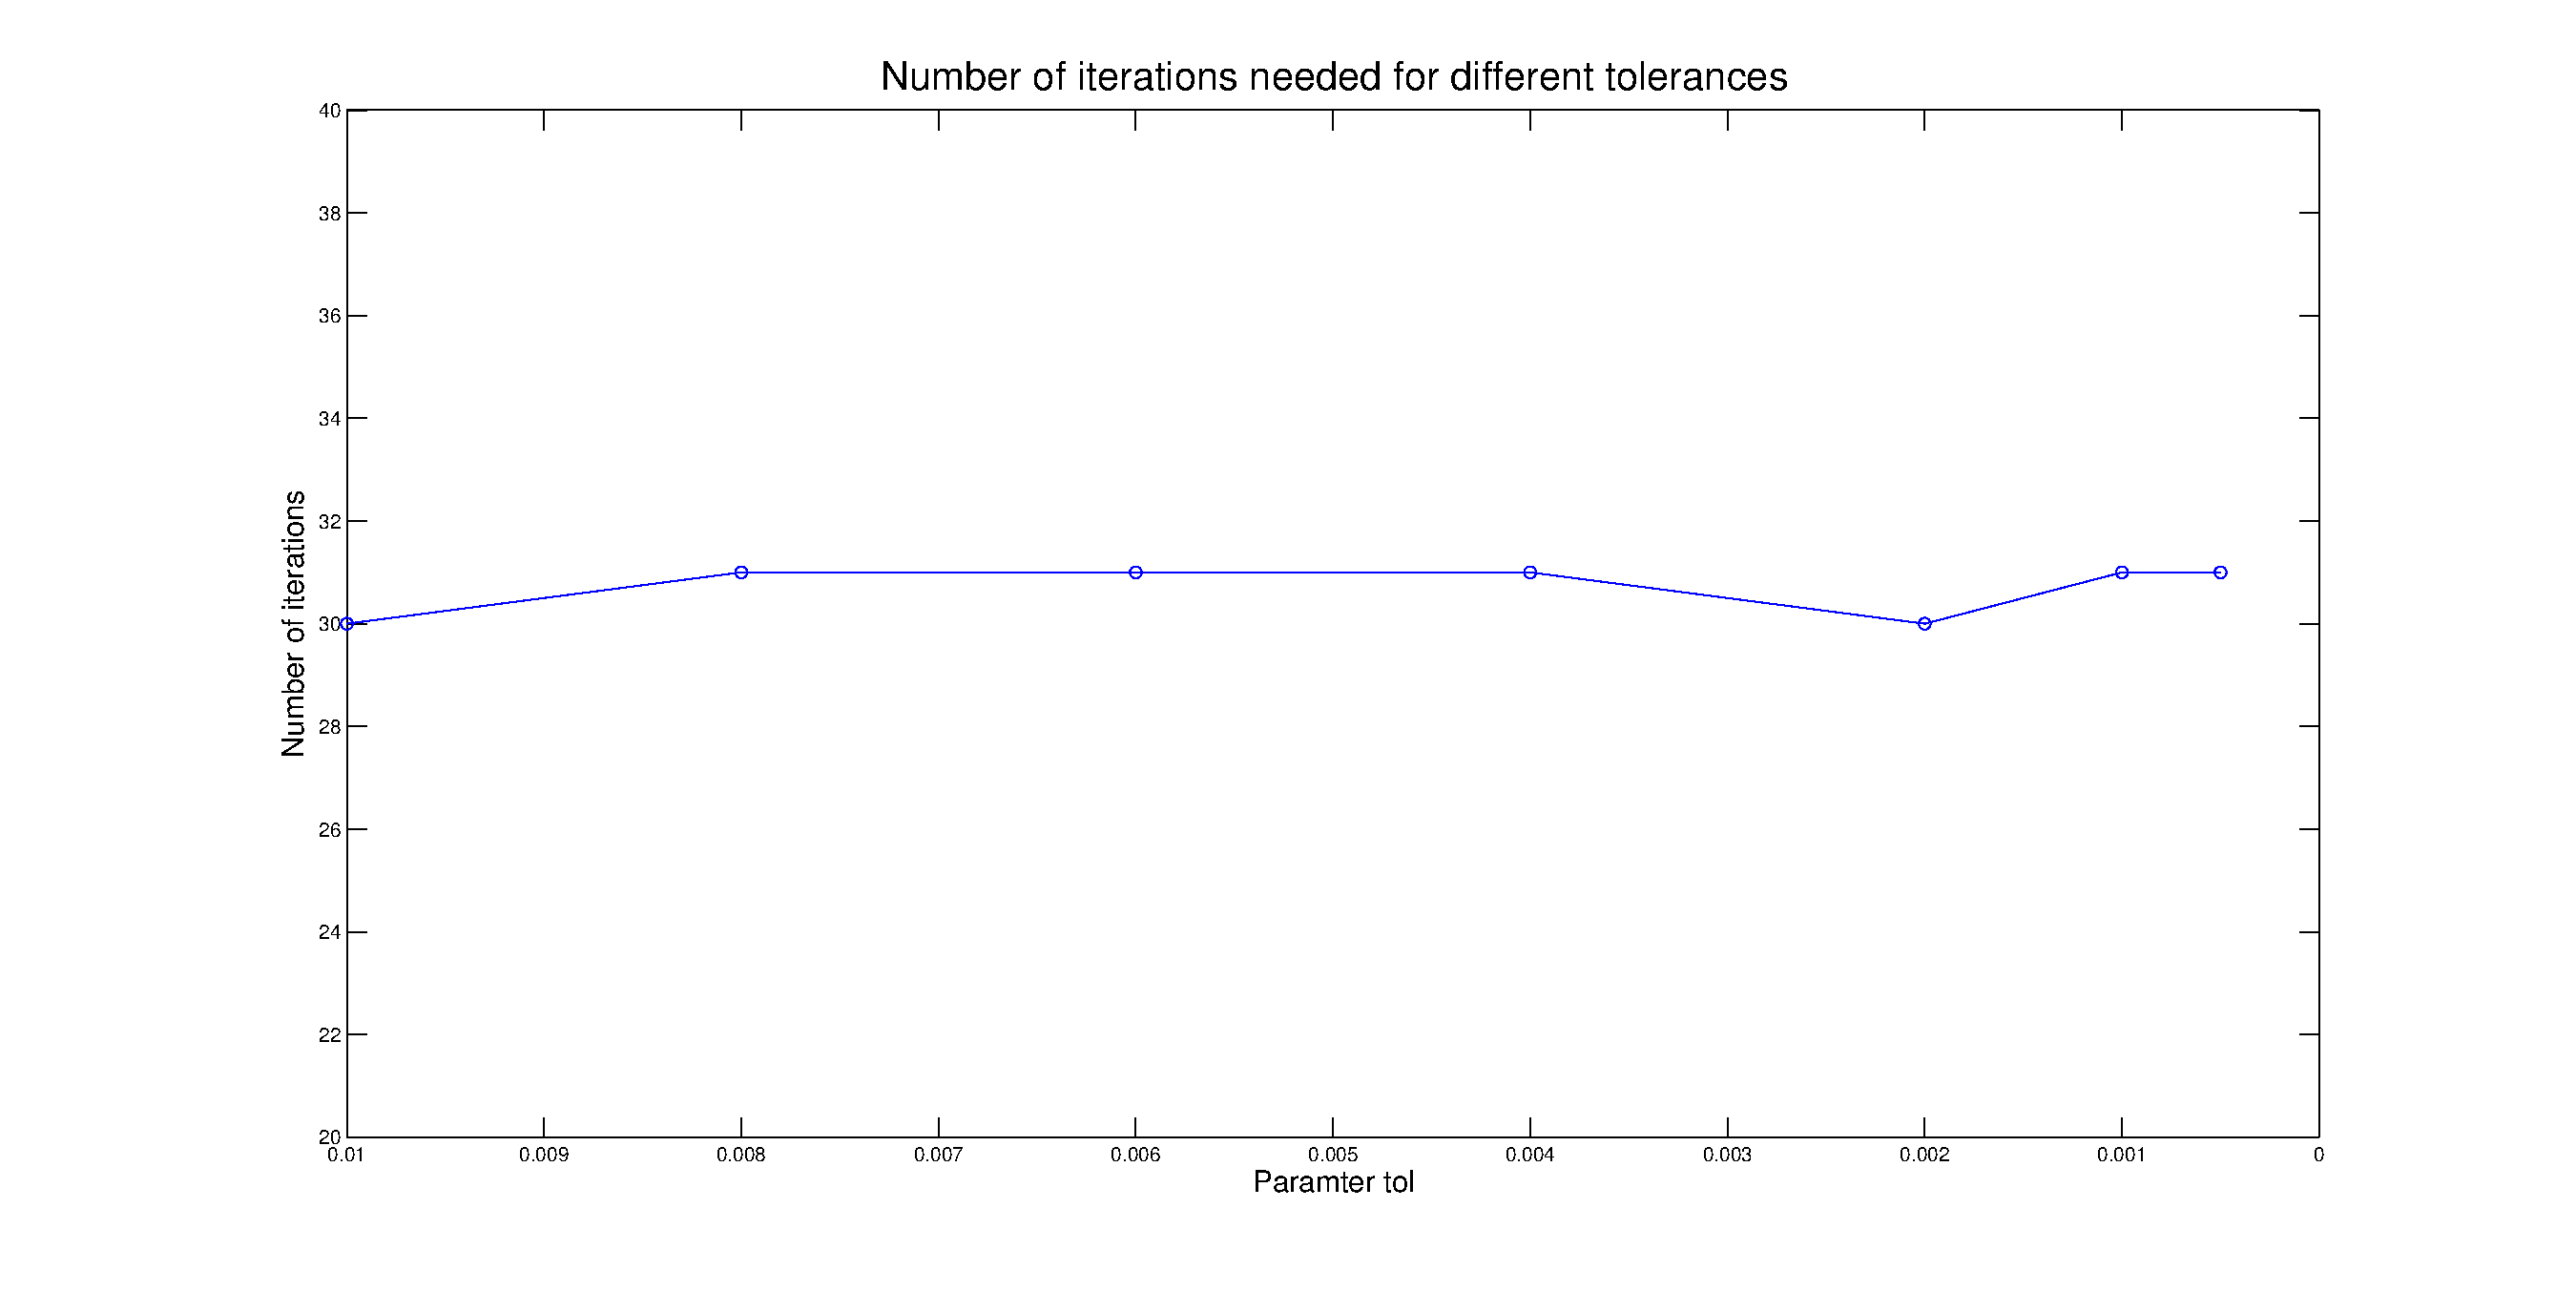
\includegraphics[scale=0.35]{Results/two_hang_iter.eps}
\caption{Number of iterations of PCG with the two scale preconditioner with a degree of interpolation $p=2$ on meshes with hanging nodes defined by the parameter $tol$.}
\label{two_hang_iter}
\end{figure}


Figure \ref{two_hang_iter} shows the number of iterations needed to reach the given tolerance with an interpolation degree $p=2$ on the different meshes presented in table \ref{two_hang_table}. We can see that the number of iterations stays roughly the same (it is either 30 or 31) for all meshes, whatever the number of hanging nodes and the value of the ratio $hang$. So we can conclude that the coarse preconditioner once again guaranties the h-independent convergence and that the number of hanging nodes does not have a great influence on the number of iterations. 

We also have to note that, for the same problem, if we use a conforming mesh, the number of iterations needed drops to 16. So even if the number of hanging nodes (absolute or relative) does not greatly influence the number of iterations, just adding one non conforming quadrant does a lot to decrease the performance of the preconditioner. We can point the fact that, as mentioned earlier, when we have hanging quadrants, we do not handle every possibilities to compute the residuals in the overlaps. We can thus see how that affects the number of iterations. 


\subsubsection{Increasing the degree of the interpolation}

\begin{figure}
\centering
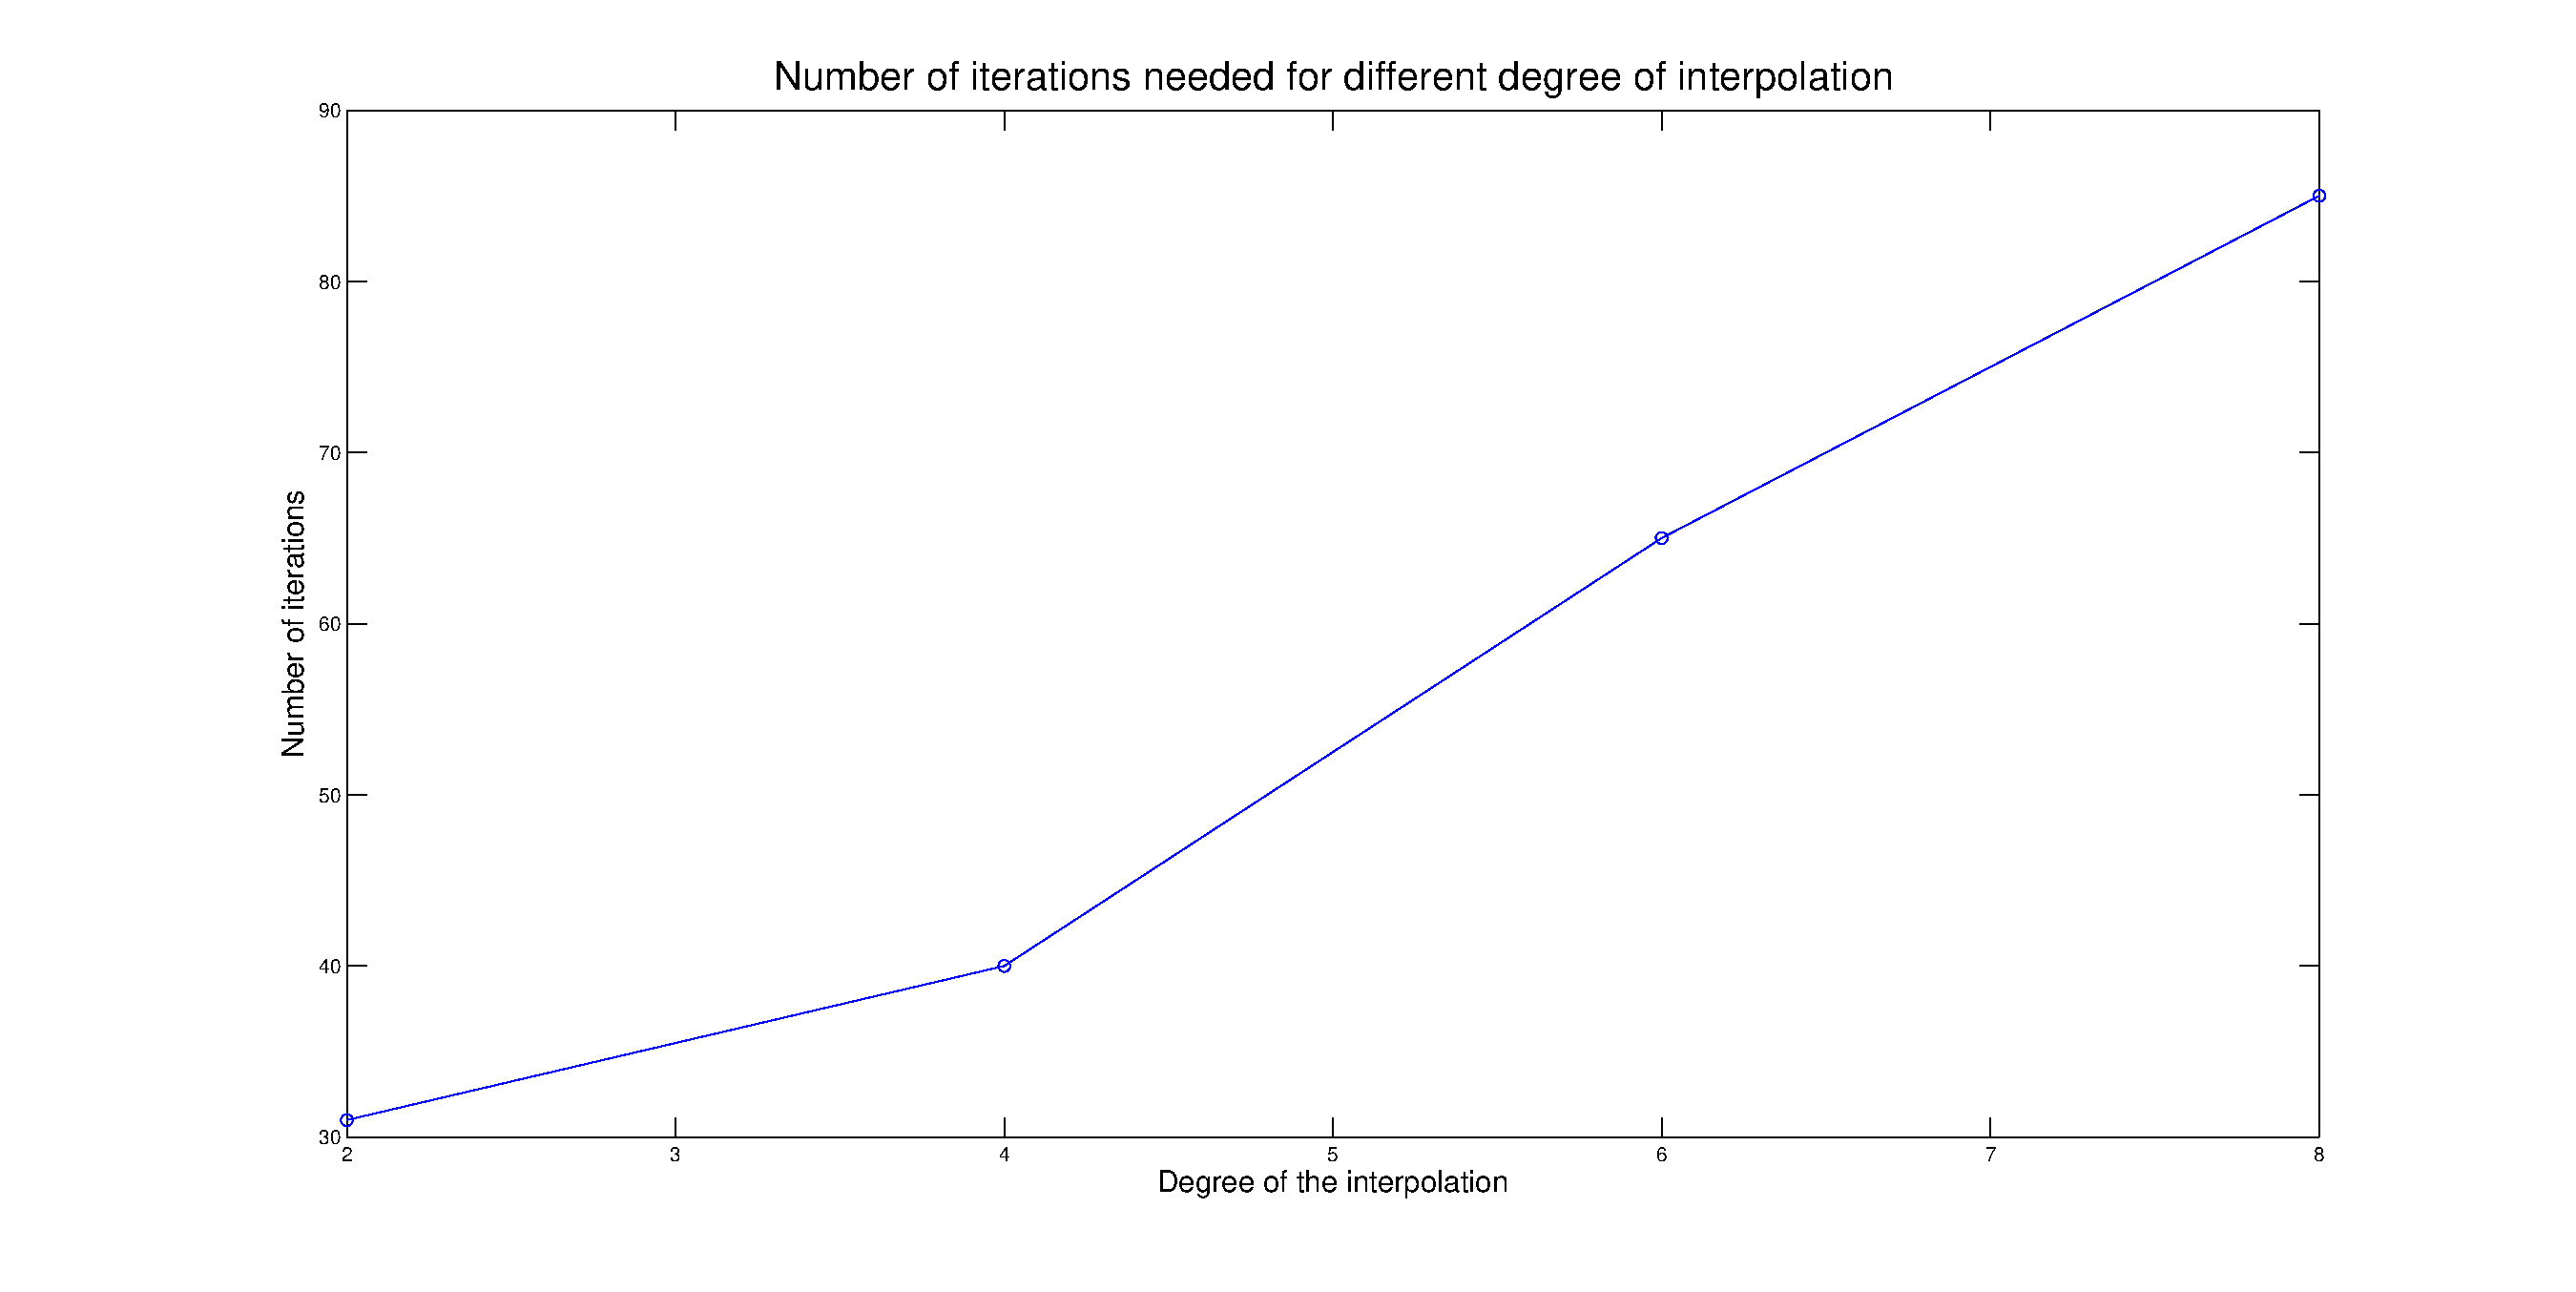
\includegraphics[scale=0.35]{Results/two_hang_deg.eps}
\caption{Number of iterations of PCG with the two scale preconditioner as a function of the degree of the interpolation used for a mesh obtained with $tol = 0.001$ in the recursive refine function.}
\label{two_hang_deg}
\end{figure}

Let us now move on to look at what happens when we increase the degree of the interpolation. We will use the mesh defined by $tol = 0.001$ and look at the number of iterations needed to reach the given tolerance for $p=2,4,6,8$. Figure \ref{two_hang_deg} shows the results. 

We can see that as we increase the degree of the interpolation, the number of iterations increases. It goes from 31 for $p=2$ to 85 iterations when $p=8$. We can see that it is quite a lot. But we also have to note that going from degree 2 to degree 8, we have also gone from $2.1\:10^5$ degrees of freedom to $3.4\:10^6$.

As in the case when we only had the fine preconditioner, several factors can be put forward to explain the increase in the number of iterations. First, when we increase the degree, the size of the overlap decreases and therefore the fine preconditioner is less effective. As mentioned in \cite{overlap_constant}, a fixed sized overlap would fix the issue. 

Second, we can say that the number of hanging nodes in the overlaps increases with the degree of the interpolation. Since we do not treat all possibilities when handling hanging quadrants, the error made is more important when we have a lot of nodes in the overlaps.


\subsection{Most efficient degree to obtain a given accuracy}

In this subsection, we will look at the best degree of interpolation $p$ to obtain a given accuracy. We will use the problem defined by \ref{eq:prob_two} and the distorted mesh using the progression tool of GMSH with $a=1.2$ that we will uniformly refine. We will also tighten the tolerance on the norm of the residual since we want the error to come from the interpolation and not from the fact that we only solve the linear system approximately. We will impose that : 

$$ \frac{||r_k||_2}{||r_0||_2} < 10^{-12} $$

Afterwards, we will compute the error committed by the discretization in the $L^2$-norm. Let us define $e^p$, the error made by using an interpolation of degree $p$, $u^p$ the solution of the discretized problem using a degree $p$, $U^p_i$ the numerical solution at the global node $i$ of the linear system that arises and $m_i$ the mass matrix associated with the integration. Then we have :  

\begin{align}
e^p &= \left( \int_\Omega (u-u^p)^2dxdy \right)^\frac{1}{2}\\
 &\approx \left( \sum_i (u(x_i,y_i)-U_i^p)^2 m_i \right)^\frac{1}{2}
\end{align}

We can note that if we refine uniformly the mesh, then $e^p$ will decrease but it will also cost us more. And for a given mesh, we have that $e^p$ decreases as $p$ increases (but it also costs us to increase the degree). So the question that arises is when is it more interesting to refine the mesh uniformly and when is it better to increase the degree of the interpolation to get the accuracy we want.

We will select degree $p$ to be the best for an accuracy of $10^{-a}$ if and only if there is a mesh such that $e^p<10^{-a}$ on this mesh and the time needed to obtain the numerical solution is smaller than for any degree on any other mesh and the same accuracy. 

\begin{figure}
\centering
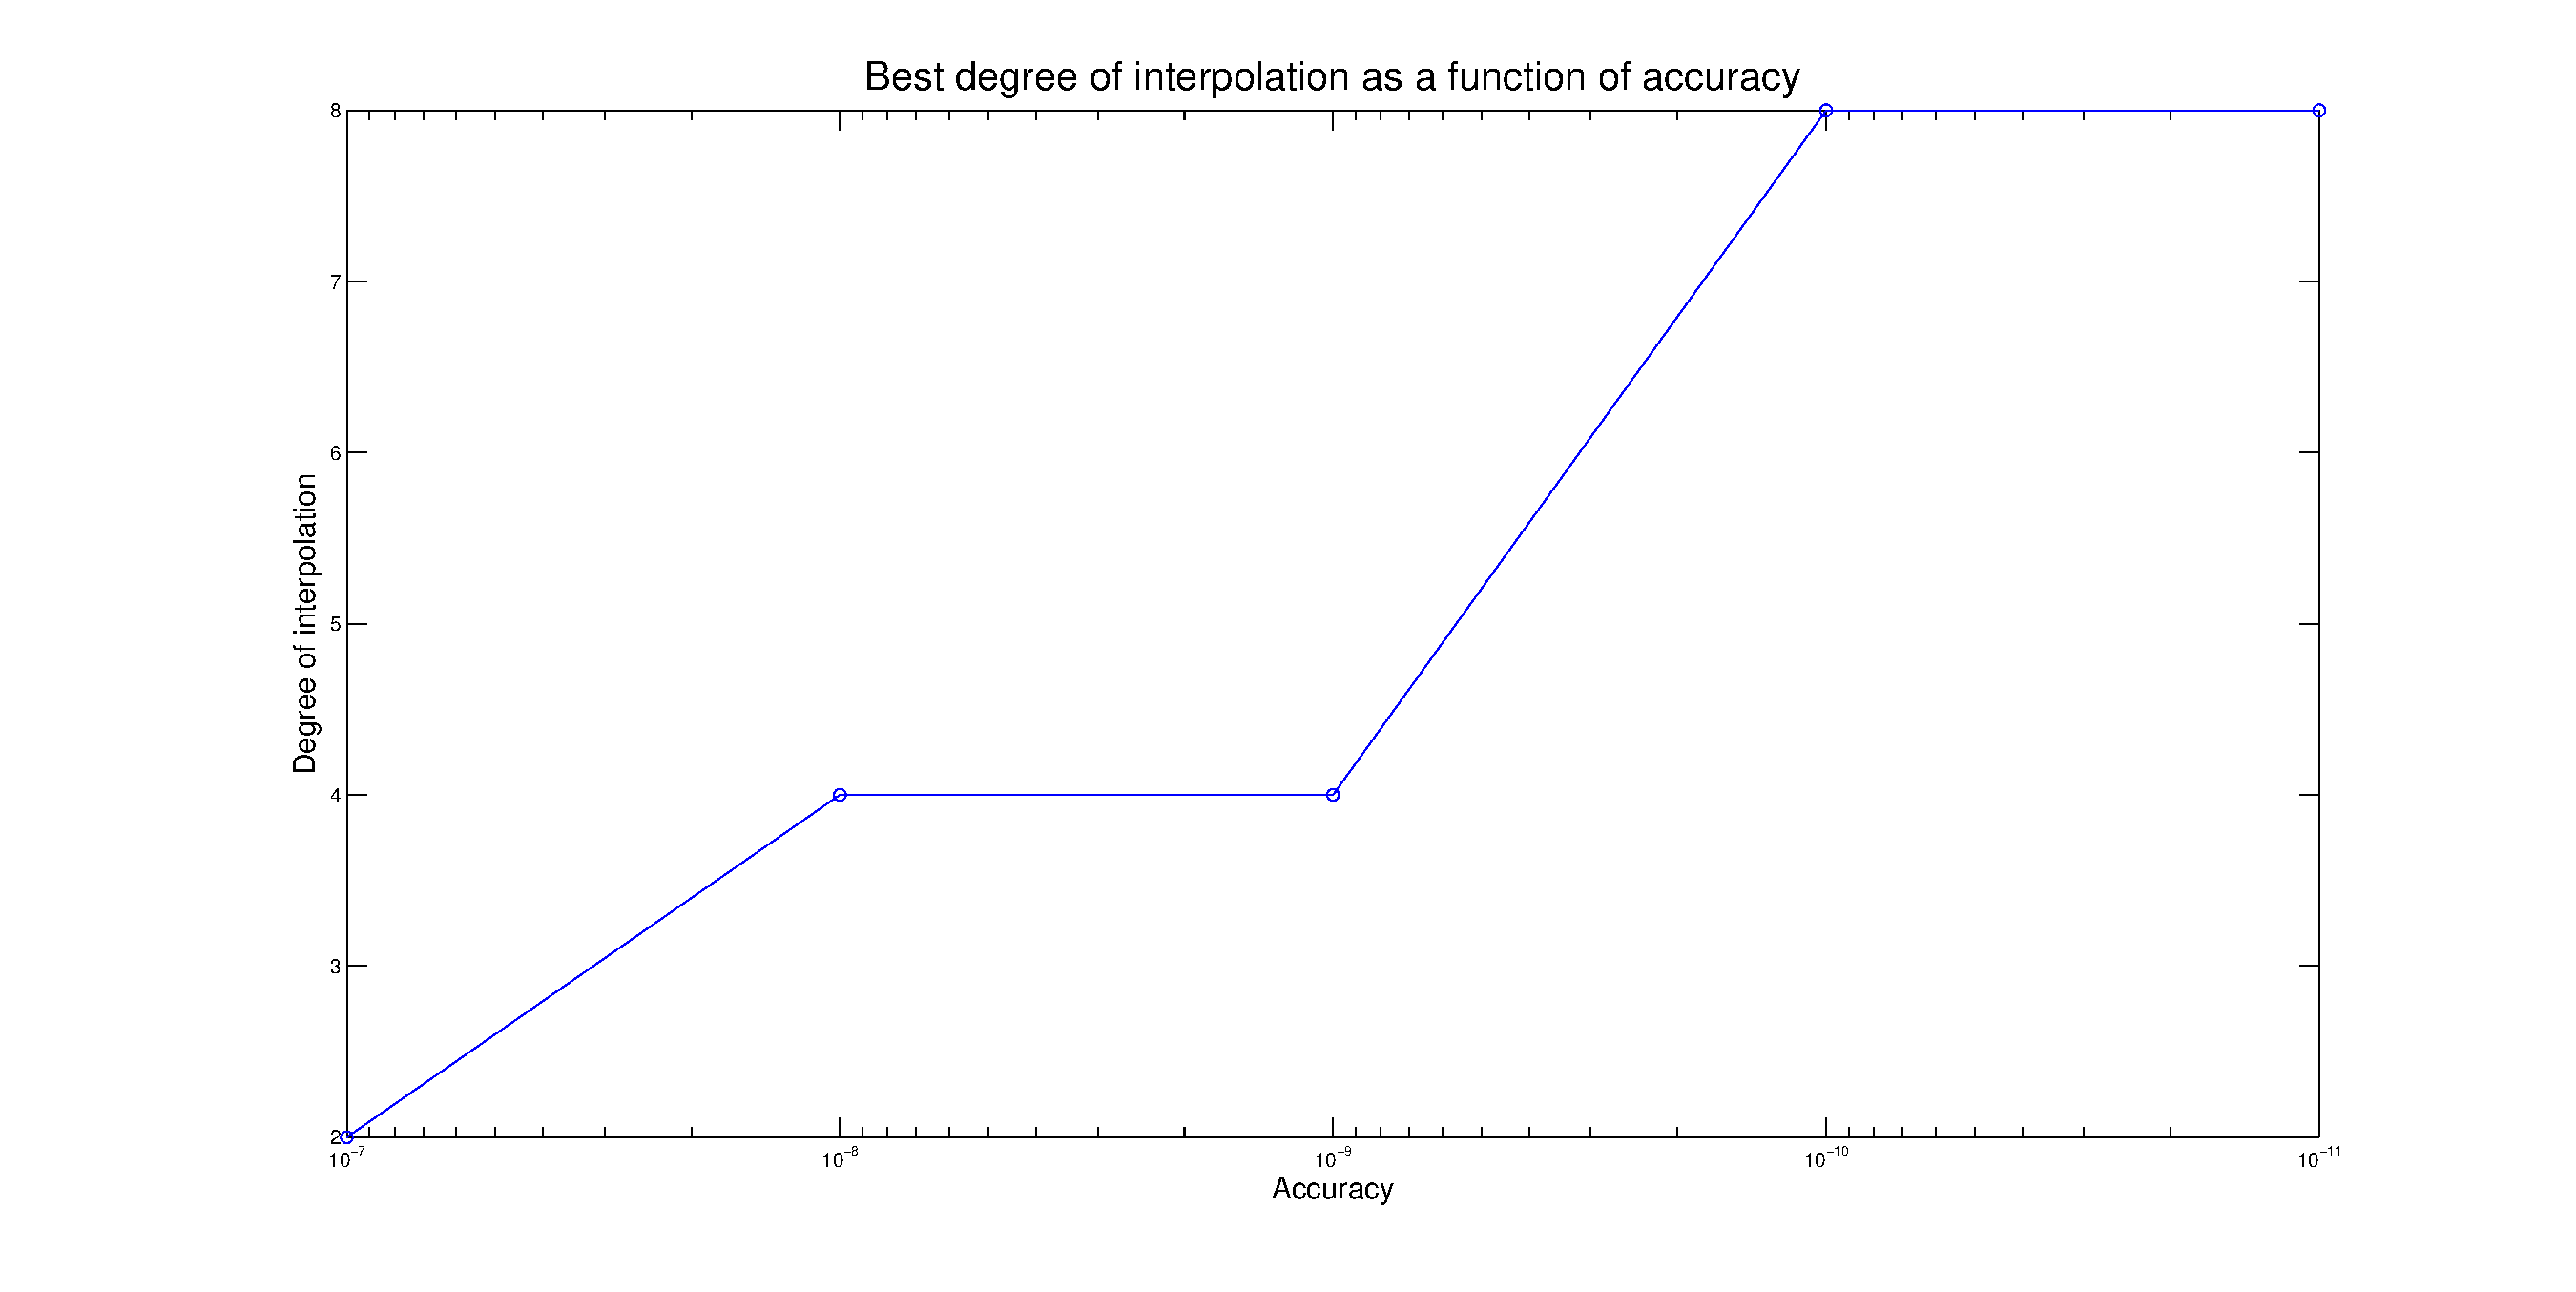
\includegraphics[scale=0.35]{Results/two_acc.eps}
\caption{Best degree of interpolation to solve problem \ref{eq:prob_two} on a distorted mesh as a function of the accuracy we want on the $L^2$-norm.}
\label{two_acc}
\end{figure}

Figure \ref{two_acc} shows the results. We can see that when the wanted accuracy is rather low (for $10^{-7}$) then it is quicker to use an order of interpolation $p=2$ because the number of iterations needed to solve the linear system is smaller than for a higher order interpolation. Moreover, the number of degrees of freedom to obtain such an accuracy is not so high as to make one iteration very long. 

On the other hand, when we want a better accuracy ($10^{-10}$, $10^{-11}$) then it is cheaper to use higher order interpolation such as $p=8$. This can be explained by the fact that, even though the number of iterations of PCG is higher (as mentioned earlier in this section), the number of degrees of freedom to obtain the wanted accuracy is much lower for $p=8$ than for the other degrees. Therefore, one iteration takes much less time and $p=8$ becomes more efficient. 

In between the two ($10^{-8}$, $10^{-9}$), we can see that the best degree is $p=4$ where we have a trade-off between the number of iterations needed to solve the system and the number of degrees of freedom.

The quantitative results presented here depend of course of the implementation, the problem to solve and the mesh used. However, we can note that the qualitative result stays true : the more accurate we want to be, the more interesting it becomes to use higher degree in the interpolation because then the number of DOF does not grow as large as it would with lower order polynomials. 





\section{Conclusion}

Let us now summarize the results given in this chapter. 

We first looked at the properties of our geometric multigrid solver. The key property of h-independent convergence has been observed for a large variety of parameters $\nu_1$ and $\nu_2$ and various meshes that were regular or distorted. The presence of hanging nodes has no influence whatsoever on the convergence of the geometric multigrid method. 

We then moved on to the PCG with only the fine scale preconditioner. Several observations were made. We saw that, even on a regular mesh where the preconditioner is optimal, increasing the number of quadrants increased the number of iterations needed. That was predicted since increasing the number of quadrants decreases the mesh size. We also noticed that we needed more iterations when the degree of interpolation $p$ grew. That was explained by the fact that the size of the overlap diminishes when $p$ increases. We then moved on to meshes with distorted quadrants and saw that we needed more iterations than in the regular case. It was to be expected since the fine preconditioner was designed to work best on quadrants aligned with the axes. Afterwards, we introduced non conforming meshes. The presence of hanging nodes also increased the number of iterations. That was explained by the fact that we do not restrict the residual exactly in the overlaps. When we increase the degree of the interpolation on a non conforming mesh, the number of iterations increases as in the conforming case. 

The coarse grid correction was then added in the preconditioner. We first tested the PCG with the two scale preconditioner on conforming meshes and saw that we obtained the h-independence thanks to the coarse preconditioner : the number of iterations stayed constant whatever the number of quadrants and the mesh size. That was true for both meshes with regular quadrants and meshes with distorted quadrants. We can however note that the number of iterations needed was greater in the case of distorted quadrants. Again, this was to be expected since the fine preconditioner works better on quadrants aligned with the axes. We then experimented on non conforming meshes. We saw that changing the absolute or the relative number of hanging nodes in the mesh had no real impact of the number of iterations. That being said, we saw that we needed more iterations when we had hanging nodes (even a few) than when we had none. We also looked at what happened when we increased the degree of the interpolation. As before, it increases with the degree $p$. The same remarks as before also apply here. 

Finally, we picked a problem and a mesh and looked at the best degree of interpolation to solve this problem, i.e. the degree which allowed us to get the solution within a given tolerance in the $L^2$-norm the quickest. We saw that at first, for a low tolerance, a low degree is best since then the fine preconditioner is cheap to compute and we can have a lot of degrees of freedom. The number if iterations of PCG is also lower for lower degrees. Then, as we tighten the tolerance, it becomes more and more attractive to use higher degrees since they allow us to keep the number of degrees of freedom down and still get a good enough approximation to be within the tolerance. The increase in the number of iteration for higher degrees is compensated by the fact that we have a lot less degrees of freedom. This means that for a given tolerance, we have a trade-off between the number of iterations of PCG and the number of degrees of freedom.  



% Bibliography
\newpage
%\bibliographystyle{unsrt}
\bibliography{sample} 


% Back cover page
\backcoverpage

\end{document}
